% !TEX TS-program = pdflatex
%%%%%%%%%%%%%%%%%%%%%%%%%%%%%%%%%%%%%%%%%%%%%%%%%%%%%%%%%%%%%%%
%
%     filename  = "YourName-Dissertation.tex",
%     version   = "1.6.5",
%     date      = "2019/07/10",
%     authors   = "Gary L. Gray,
%     copyright = "Gary L. Gray",
%     address   = "Engineering Science and Mechanics,
%                  212 Earth & Engineering Sciences Bldg.,
%                  Penn State University,
%                  University Park, PA 16802,
%                  USA",
%     telephone = "814-863-1778",
%     email     = "gray@psu.edu",
%
%%%%%%%%%%%%%%%%%%%%%%%%%%%%%%%%%%%%%%%%%%%%%%%%%%%%%%%%%%%%%%%
% Change History:
% The change history can be found in the accompanying document
% entitled "YourName-Dissertation Template Change History.md".
%%%%%%%%%%%%%%%%%%%%%%%%%%%%%%%%%%%%%%%%%%%%%%%%%%%%%%%%%%%%%%%
%
% This is a template file to help get you started using the
% psuthesis.cls for theses and dissertations at Penn State
% University. You will, of course, need to put the
% psuthesis.cls file someplace that LaTeX will find it.
%
% I have set up a directory structure that I find to be clean
% and convenient. You can readjust it to suit your tastes. In
% fact, the structure used by our students is even a little
% more involved and commands are defined to point to the
% various directories.
%
% This document has been set up to be typeset using pdflatex.
% About the only thing you will need to change if typesetting
% using latex is the \DeclareGraphicsExtensions command.
%
% The psuthesis document class uses the same options as the
% book class. In addition, it requires that you have the
% ifthen, calc, setspace, and tocloft packages.
%
% The first additional option specifies the degree type. You
% can choose from:
%	Ph.D. using class option <phd>
%	M.S. using class option <ms>
%	M.Eng. using class option <meng>
%	M.A. using class option <ma>
%	B.S. using class option <bs>
%	B.A. using class option <ba>
%	Honors from the Schreyer Honors College <schreyer>
%
% The second additional option inlinechaptertoc determines
% the formatting of the Chapter entries in the Table of
% Contents. The default sets them as two-line entries (try it).
% If you want them as one-line entries, issue the
% inlinechaptertoc option.
%
%
% The option option twoha should be used if you are earning
% interdisciplanary honors and thus have two honors advisors.
%
% The class option ``secondthesissupervisor'' should be used
% for baccalaureate honors degrees if you have a second
% Thesis Supervisor.
%
% The vita is only included with the phd option and it is
% placed at the end of the thesis. The permissions page is only
% included with the ms, meng, and ma options.
%%%%%%%%%%%%%%%%%%%%%%%%%%%%%%%%%%%%%%%%%%%%%%%%%%%%%%%%%%%%%%%
% Only one of the following lines should be used at a time.
% Doctoral students.
\documentclass[phd,12pt]{psuthesis}
% Masters students
%\documentclass[ms,12pt]{psuthesis}
% Bachelors students in the Schreyer Honors College.
%\documentclass[bs,schreyer,12pt]{psuthesis}
% Bachelors students in the Schreyer Honors College & Engineering Science.
%\documentclass[bs,schreyer,esc,twoha,12pt]{psuthesis}
% Bachelors students in Engineering Science.
%\documentclass[bs,esc,12pt]{psuthesis}

\usepackage[T1]{fontenc}
\usepackage{lmodern}
\usepackage{textcomp}
\usepackage{microtype}
%%%%%%%%%%%%%%%%%%%%%%%%
%%%%%%中文引用%%%%%%
% \usepackage{CJKutf8}
% \AtBeginDocument{\begin{CJK}{UTF8}{gbsn}}

% \AtEndDocument{\end{CJK}}
%%%%%%%%%%%%%%%%%%%%%%%%%%%
% Packages I like to use. %
%%%%%%%%%%%%%%%%%%%%%%%%%%%
\usepackage{amsmath}
\usepackage{amssymb}
%\usepackage{amsthm}
%\usepackage{exscale}
%\usepackage[mathscr]{eucal}
%\usepackage{bm}
\usepackage{multirow}
\usepackage{booktabs}
\usepackage{caption}
\usepackage{subfigure}
\usepackage{eqlist} % Makes for a nice list of symbols.
\usepackage[nosepfour,warning,np,debug,autolanguage]{numprint}
\usepackage{acro}
\usepackage{booktabs}
\usepackage[final]{graphicx}
\usepackage[dvipsnames]{color}
\DeclareGraphicsExtensions{.pdf, .jpg}
\usepackage{float}
\usepackage{url}
\usepackage{longtable}
% http://www.tex.ac.uk/cgi-bin/texfaq2html?label=citesort
\usepackage{cite}

\usepackage{titlesec}

%%%%%%%%%%%%%%%%%%%%%%%%%%%%%%%
% Use of the hyperref package %
%%%%%%%%%%%%%%%%%%%%%%%%%%%%%%%
%
% This is optional and is included only for those students
% who want to use it.
%
% To the hyperref package, uncomment the following line:
%\usepackage{hyperref}
%
% Note that you should also uncomment the following line:
%\renewcommand{\theHchapter}{\thepart.\thechapter}
%
% to work around some a problem hyperref has with the fact
% the psuthesis class has unnumbered pages after which page
% counters are reset.

% Set the baselinestretch using the setspace package.
% The LaTeX Companion claims that a \baselinestretch of
% 1.24 gives one-and-a-half line spacing, which is allowed
% by the PSU thesis office. As of October 18, 2013, the Graduate
% School states ``The text of an eTD may be single-, double- or
% one- and-a-half-spaced.'' Go nuts!
\setstretch{1.24}


%%%%%%%%%%%%%%%%%%%%%%%%%%%%%%%%%%%%
% SPECIAL SYMBOLS AND NEW COMMANDS %
%%%%%%%%%%%%%%%%%%%%%%%%%%%%%%%%%%%%
% Place user-defined commands below.

% Define the \acro command.
\makeatletter
\newif\ifFirstPar       \FirstParfalse
\def\smc{\sc}
\def\ninepoint{\small}
\DeclareRobustCommand\SMC{%
  \ifx\@currsize\normalsize\small\else
   \ifx\@currsize\small\footnotesize\else
    \ifx\@currsize\footnotesize\scriptsize\else
     \ifx\@currsize\large\normalsize\else
      \ifx\@currsize\Large\large\else
       \ifx\@currsize\LARGE\Large\else
        \ifx\@currsize\scriptsize\tiny\else
         \ifx\@currsize\tiny\tiny\else
          \ifx\@currsize\huge\LARGE\else
           \ifx\@currsize\Huge\huge\else
            \small\SMC@unknown@warning
 \fi\fi\fi\fi\fi\fi\fi\fi\fi\fi
}
\newcommand\SMC@unknown@warning{\TBWarning{\string\SMC: unrecognised
    text font size command -- using \string\small}}
\newcommand\textSMC[1]{{\SMC #1}}
\newcommand\acro[1]{\textSMC{#1}\@}

\makeatother

% command for vectors
\newcommand{\bv}[1]{\ensuremath{\vec{#1}}}
% command for unit vectors
\newcommand{\uv}[2][blank]{%
\ifthenelse{\equal{#1}{blank}}%
{\ensuremath{\hat{u}_{#2}}}%
{}%
%
\ifthenelse{\equal{#1}{.}}%
{\ensuremath{\dot{\hat{u}}_{#2}}}%
{}%
%
\ifthenelse{\equal{#1}{'}}%
{\ensuremath{\hat{u}'_{#2}}}%
{}%
}
\newcommand{\ui}{\ensuremath{\hat{\imath}}}
\newcommand{\uj}{\ensuremath{\hat{\jmath}}}
\newcommand{\uk}{\ensuremath{\hat{k}}}



%%%%%%%%%%%%%%%%%%%%%%%%%%%%%%%%%%%%%%%%%
% Renewed Float Parameters              %
% (Makes floats fit better on the page) %
%%%%%%%%%%%%%%%%%%%%%%%%%%%%%%%%%%%%%%%%%
\renewcommand{\floatpagefraction}{0.85}
\renewcommand{\topfraction}      {0.85}
\renewcommand{\bottomfraction}   {0.85}
\renewcommand{\textfraction}     {0.15}

% ----------------------------------------------------------- %

%%%%%%%%%%%%%%%%
% FRONT-MATTER %
%%%%%%%%%%%%%%%%
% Title
\title{Central and Local Governmental Fiscal Behavior under Fiscal Federalism---An Analysis with Asymmetric Setting}

% Author and Department
\author{Yan Hao}
\dept{School of Public Affairs}
% the degree will be conferred on this date
\degreedate{June 2023}
% year of your copyright
\copyrightyear{2023}

% This command is used for students submitting a thesis to the
% Schreyer Honors College and for students in Engineering Science.
% The argument of this command should contain every after the word
% ``requirements'' that appears on the title page. This provides the
% needed flexibility for all the degree types.
\bachelorsdegreeinfo{for a doctoral degree \\ in public administration \\ with honors in public finance}

% This is the document type. For example, this could also be:
%	Comprehensive Document
%	Thesis Proposal
\documenttype{Thesis}
%\documenttype{Dissertation}
%\documenttype{Comprehensive Document}


% This will generally be The Graduate School, though you can
% put anything in here to suit your needs.
\submittedto{The Graduate School}

% This is the college to which you are submitting the
% thesis/dissertation.
\collegesubmittedto{School of Public Affairs}


%%%%%%%%%%%%%%%%%%
% Signatory Page %
%%%%%%%%%%%%%%%%%%
% You can have up to 7 committee members, i.e., one advisor
% and up to 6 readers.
%
% Begin by specifying the number of readers.
\numberofreaders{3}

% For baccalaureate honors degrees, enter the name of your
% honors advisor below.
%\honorsadvisor{Odd Stalebrink}
%{Associate Professor of Public Administration}
%\honorsadvisortwo{Honors P. Advisor, Jr.}
%{Professor of Engineering Science and Mechanics}
 
% For baccalaureate honors degrees, if you have a second
% Thesis Supervisor, enter his or her name below.
%\secondthesissupervisor{Second T. Supervisor}

% For baccalaureate honors degrees, certain departments
% (e.g., Engineering Science and Mechanics) require the
% signature of the department head. In that case, enter the
% name and title of your department head below.
%\escdepthead{Department Q. Head}
%\escdeptheadtitle{P. B. Breneman Chair and Professor 
%of Engineering Science and Mechanics
%}

% Input reader information below. The optional argument, which
% comes first, goes on the second line before the name.
\advisor[Thesis Advisor][Chair of Committee]
		{Odd Stalebrink}
		{Associate Professor of Public Administration}

\readerone[Dissertation Committee Member]
			{Younhee Kim}
			{Associate Professor of Public Administration}

\readertwo[Dissertation Committee Member]
			{Daniel J. Mallinson}
			{Associate Professor of Public Administration}

\readerthree[Dissertation Committee Member]
			{David Argente}
			{Assistant Professor of Economics}
%%%%%%%%%%%%%%%%%%%%%%%%%%%%%%%%%%%%%%%%%%%%%%%%%
%\readerfour[Optional Title Here]
%			{Reader Name}
%{Professor of SomeThing}
%
%\readerfive[Optional Title Here]
%			{Reader Name}
%			{Professor of SomeThing}
%%%%%%%%%%%%%%%%%%%%%%%%%%%%%%%%%%%%%%%%%%%%%%%%
% Format the Chapter headings using the titlesec package.
% You can format section headings and the like here too.
\definecolor{gray75}{gray}{0.75}
\newcommand{\hsp}{\hspace{15pt}}
\titleformat{\chapter}[display]{\fontsize{30}{30}\selectfont\bfseries\sffamily}{Chapter \thechapter\hsp\textcolor{gray75}{\raisebox{3pt}{|}}}{0pt}{}{}

\titleformat{\section}[block]{\Large\bfseries\sffamily}{\thesection}{12pt}{}{}
\titleformat{\subsection}[block]{\large\bfseries\sffamily}{\thesubsection}{12pt}{}{}


% Makes use of LaTeX's include facility. Add as many chapters
% and appendices as you like.
\includeonly{%
Chapter-1/Chapter-1,%
Chapter-2/Chapter-2,%
Chapter-3/Chapter-3,%
Chapter-4/Chapter-4,%
%Chapter-5/Chapter-5,%
%Chapter-6/Chapter-6,%
Appendix-A/Appendix-A,%
Appendix-B/Appendix-B,%
Appendix-C/Appendix-C,%
Appendix-D/Appendix-D,%
Appendix-E/Appendix-E%
}

\usepackage{listings}
%%%%%%%%%%%%%%%%%
% THE BEGINNING %
%%%%%%%%%%%%%%%%%
\begin{document}
\pagestyle{fancy}
\fancyhead[L,C,R]{}
\fancyfoot[L,R]{}
\fancyfoot[C]{\thepage}
\renewcommand{\headrulewidth}{0pt}
\renewcommand{\footrulewidth}{0pt}
%%%%%%%%%%%%%%%%%%%%%%%%
% Preliminary Material %
%%%%%%%%%%%%%%%%%%%%%%%%
% This command is needed to properly set up the frontmatter.
\frontmatter

%%%%%%%%%%%%%%%%%%%%%%%%%%%%%%%%%%%%%%%%%%%%%%%%%%%%%%%%%%%%%%
% IMPORTANT
%
% The following commands allow you to include all the
% frontmatter in your thesis. If you don't need one or more of
% these items, you can comment it out. Most of these items are
% actually required by the Grad School -- see the Thesis Guide
% for details regarding what is and what is not required for
% your particular degree.
%%%%%%%%%%%%%%%%%%%%%%%%%%%%%%%%%%%%%%%%%%%%%%%%%%%%%%%%%%%%%%
% !!! DO NOT CHANGE THE SEQUENCE OF THESE ITEMS !!!
%%%%%%%%%%%%%%%%%%%%%%%%%%%%%%%%%%%%%%%%%%%%%%%%%%%%%%%%%%%%%%

% Generates the title page based on info you have provided
% above.
\psutitlepage

% Generates the committee page -- this is bound with your
% thesis. If this is an baccalaureate honors thesis, then
% comment out this line.
\psucommitteepage

% Generates the abstract. The argument should point to the
% file containing your abstract. 
\thesisabstract{SupplementaryMaterial/Abstract}

% Generates the Table of Contents
\thesistableofcontents

% Generates the List of Figures
\begin{singlespace}
    \renewcommand{\listfigurename}{\sffamily\Huge List of Figures}
    \setlength{\cftparskip}{\baselineskip}
    \addcontentsline{toc}{chapter}{List of Figures}
    %\fancypagestyle{plain}{%
    %\fancyhf{} % clear all header and footer fields
    %\fancyfoot[C]{\thepage}} % except the center
    \listoffigures
\end{singlespace}
\clearpage

% Generates the List of Tables
\begin{singlespace}
    \renewcommand{\listtablename}{\sffamily\Huge List of Tables}
    \setlength{\cftparskip}{\baselineskip}
    \addcontentsline{toc}{chapter}{List of Tables}
    \listoftables
\end{singlespace}
\clearpage

% Generates the List of Symbols. The argument should point to
% the file containing your List of Symbols. 
\thesislistofsymbols{SupplementaryMaterial/ListOfSymbols}

% Generates the Acknowledgments. The argument should point to
% the file containing your Acknowledgments. 
\thesisacknowledgments{SupplementaryMaterial/Acknowledgments}

% Generates the Epigraph/Dedication. The first argument should
% point to the file containing your Epigraph/Dedication and
% the second argument should be the title of this page. 
%\thesisdedication{SupplementaryMaterial/Dedication}{Dedication}



%%%%%%%%%%%%%%%%%%%%%%%%%%%%%%%%%%%%%%%%%%%%%%%%%%%%%%
% This command is needed to get the main part of the %
% document going.                                    %
%%%%%%%%%%%%%%%%%%%%%%%%%%%%%%%%%%%%%%%%%%%%%%%%%%%%%%
\thesismainmatter

%%%%%%%%%%%%%%%%%%%%%%%%%%%%%%%%%%%%%%%%%%%%%%%%%%
% This is an AMS-LaTeX command to allow breaking %
% of displayed equations across pages. Note the  %
% closing the "}" just before the bibliography.  %
%%%%%%%%%%%%%%%%%%%%%%%%%%%%%%%%%%%%%%%%%%%%%%%%%%
\allowdisplaybreaks{
    %\pagestyle{fancy}
    %\fancyhead{}
    %
    %%%%%%%%%%%%%%%%%%%%%%
    % THE ACTUAL CONTENT %
    %%%%%%%%%%%%%%%%%%%%%%
    % Chapters
    % !TEX root = ../Yan Hao-Dissertation.tex

\chapter{Introduction} \label{chapter1:Introduction}

\section{About Fiscal Federalism}
The field of fiscal federalism studies how to divide responsibilities (including finances) among federal, state, and local governments to improve economic efficiency and achieve various public policy objectives.Determining the optimal division of responsibilities and funding is difficult because of varying subjective views about what the role of government should be. As a result, fiscal federalism research generally renders no judgment on the proper level of total government intervention or what types of services governments should provide. The research focuses instead on how responsibilities are assigned across multiple layers of government once policymakers have decided to implement a given policy, and what trade-offs may be involved in administering it. To be more specific, Central and local governments have their own way to generate revenue and supply public goods and services separately. Besides, central government compensate the low income subnational government by doing transfer payments,which is so called intergovernmental transfer, so local governments especially the low-income local government still got the ability to supply the necessary public goods and services. To summarize, central and local governments got the ability to collect the revenue so to supply the necessary public goods and services with the consideration to achieve the political intention. Depend on the general fiscal federalism setting, I'll give an overall view of the fiscal federalism structure in the rest of this chapter. Three key points are vital for the understanding: the revenue source for different levels of government, the public service responsibilities,and the financial connection between central and subnational governments, as is shown in Figure \ref*{Figure 1.1}

\begin{figure}[htb]
    \centering
    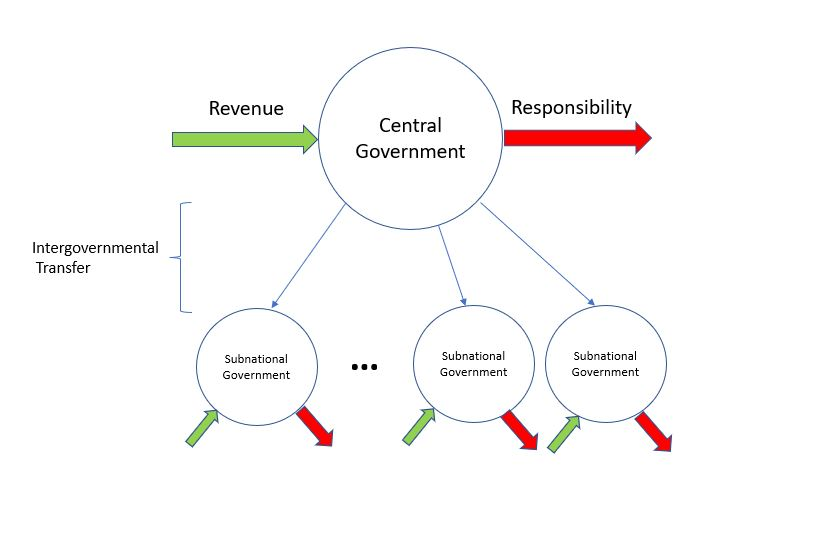
\includegraphics[scale=0.7]{Chapter-1/Figures/fiscal federalism.JPG}
    \caption[Fiscal Federalism Structure]{Fiscal Federalism Structure
        \texttt{} }
    \label{Figure 1.1}
\end{figure}

For the following part of this chapter, I'll give a basic introduction about the fiscal federalism structure in USA, to be more specific, I'll describe the revenue and responsibilities of different levels of governments, and the intergovernmental transfer between different levels of governments.



\subsection{Fiscal Federalism Structure in America}
\subsubsection{Revenue and Responsibilities of different levels governments}
The United States constitution stipulated that states keep the remaining rights, which means except for the clear defined rights that federal government have, states government keep the undefined rights. Besides, the constitution set no instruction about the responsibilities between state and local governments. This feature combined with the fact that America is a huge country with rich diversity lead to an interesting administrative fact: the responsibilities of state governments in each states are not identical. Within each states, the local governments form up their responsibilities based on the actual needs, thus the local governments are not identical neither. Thus the follow introduction are not describing the administrative reality precisely, but are introducing the general structure.

Under current fiscal federalism system in America, federal, state and local governments rely on different source of income, have different function in supplying the public good and federal government reimburse the state and local government through intergovernmental transfer. On revenue side, from the breakdown of the source of revenue of fiscal year 2019, 50\% of the federal revenue comes from the individual income tax, 7\% from corporate income tax, 36\% is social insurance or payroll tax. On the other hand, on state and local level, intergovernmental transfer accounts for more than 30 percent on average, followed by sales taxes and property tax.
%%%%%%%%%
\begin{figure}[H]
    \centering  %居中
    \subfigure[Source of Federal General Revenue]{   %第一张子图
        \begin{minipage}{7cm}
            \centering    %子图居中
            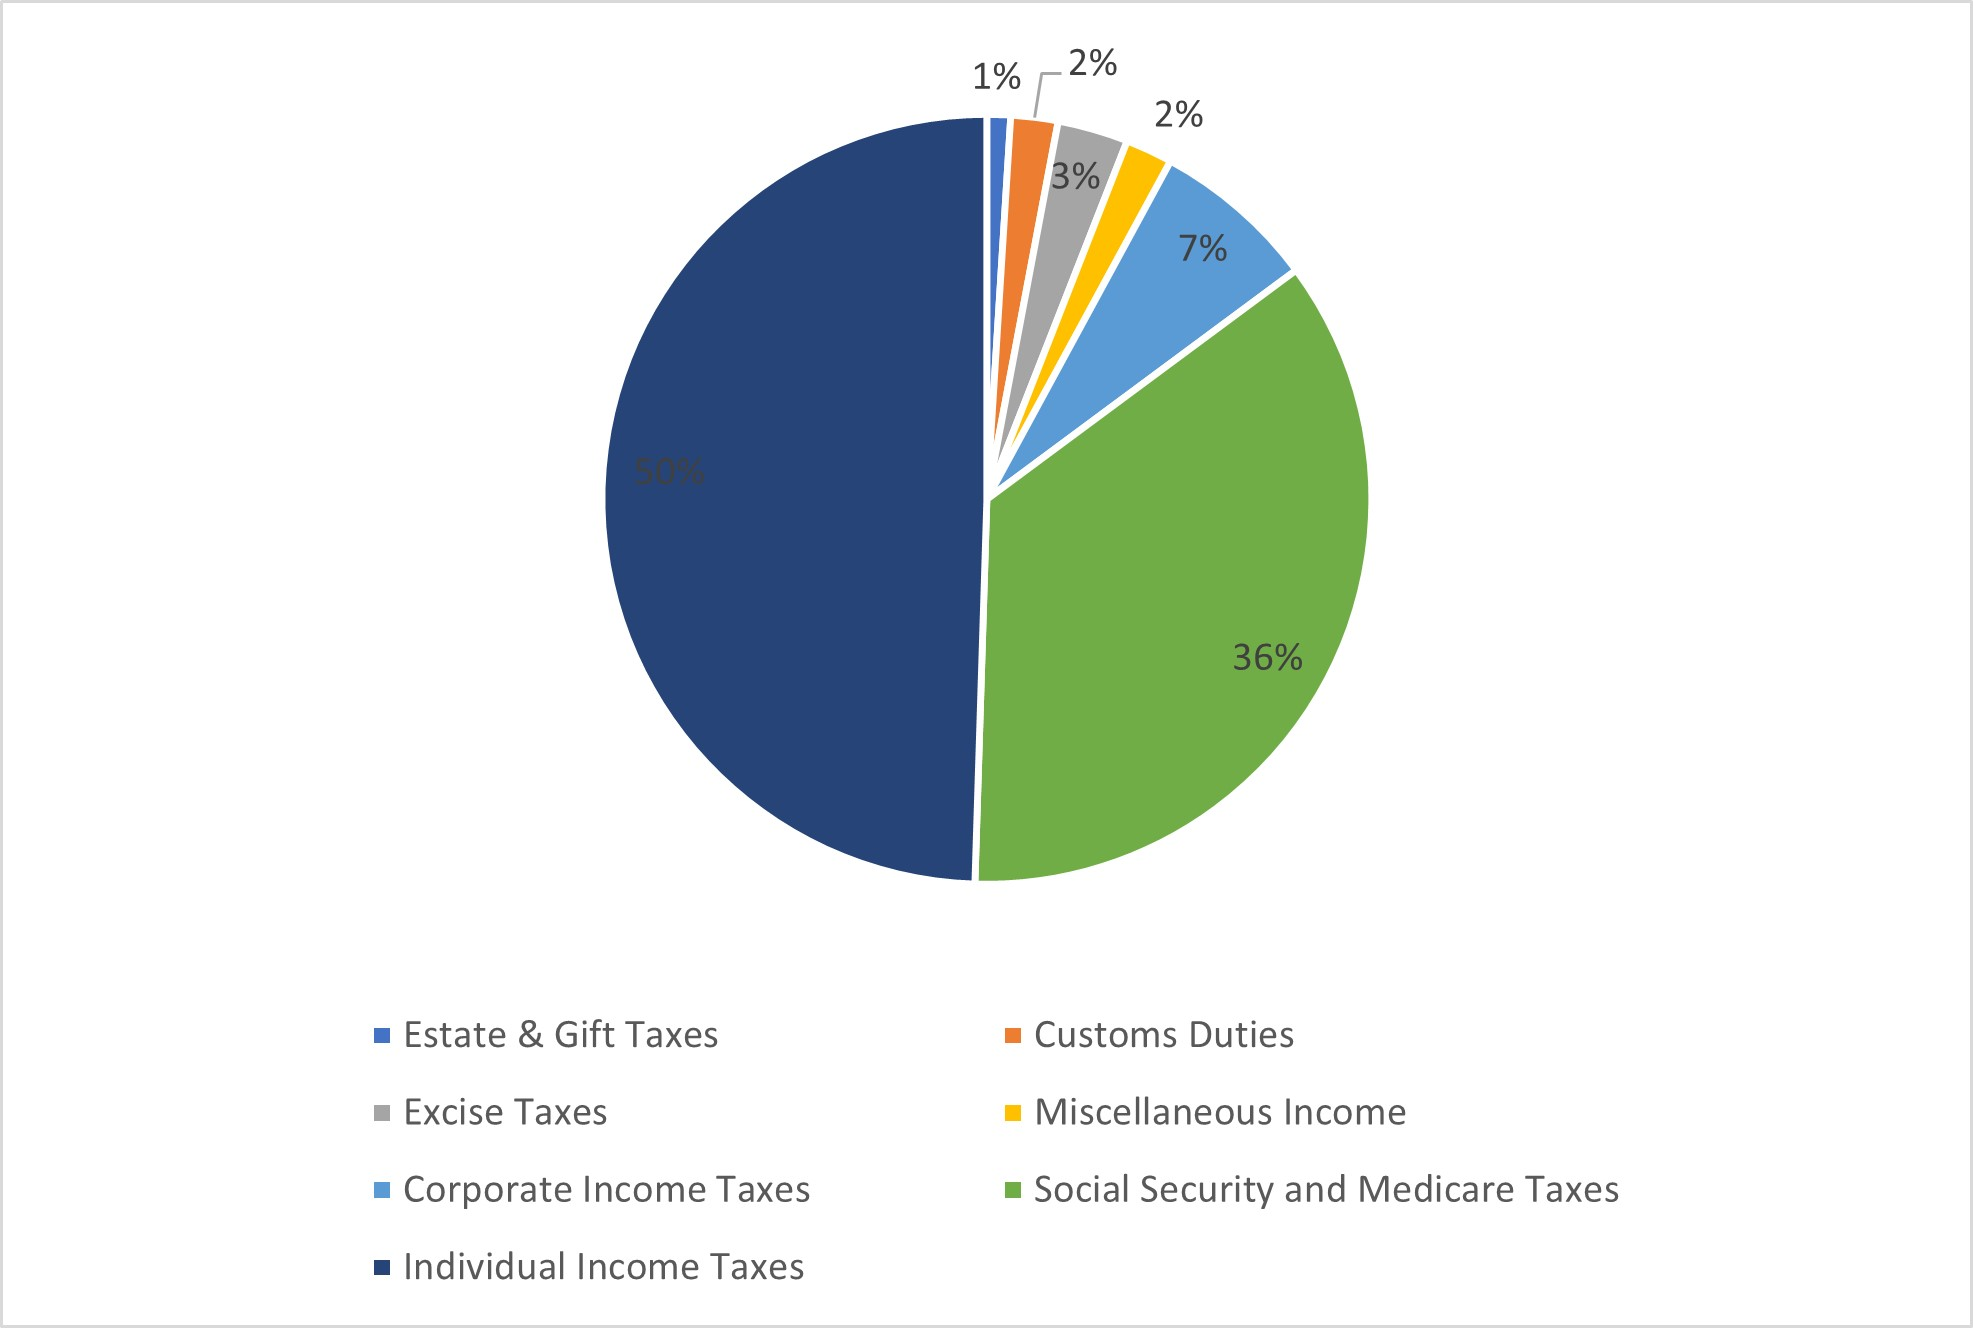
\includegraphics[scale=0.37]{Chapter-1/Figures/source of federal general revenue.jpg}  %以pic.jpg的0.5倍大小输出
        \end{minipage}
    }
    \subfigure[Source of State General Revenue]{ %第二张子图
        \begin{minipage}{7cm}
            \centering    %子图居中
            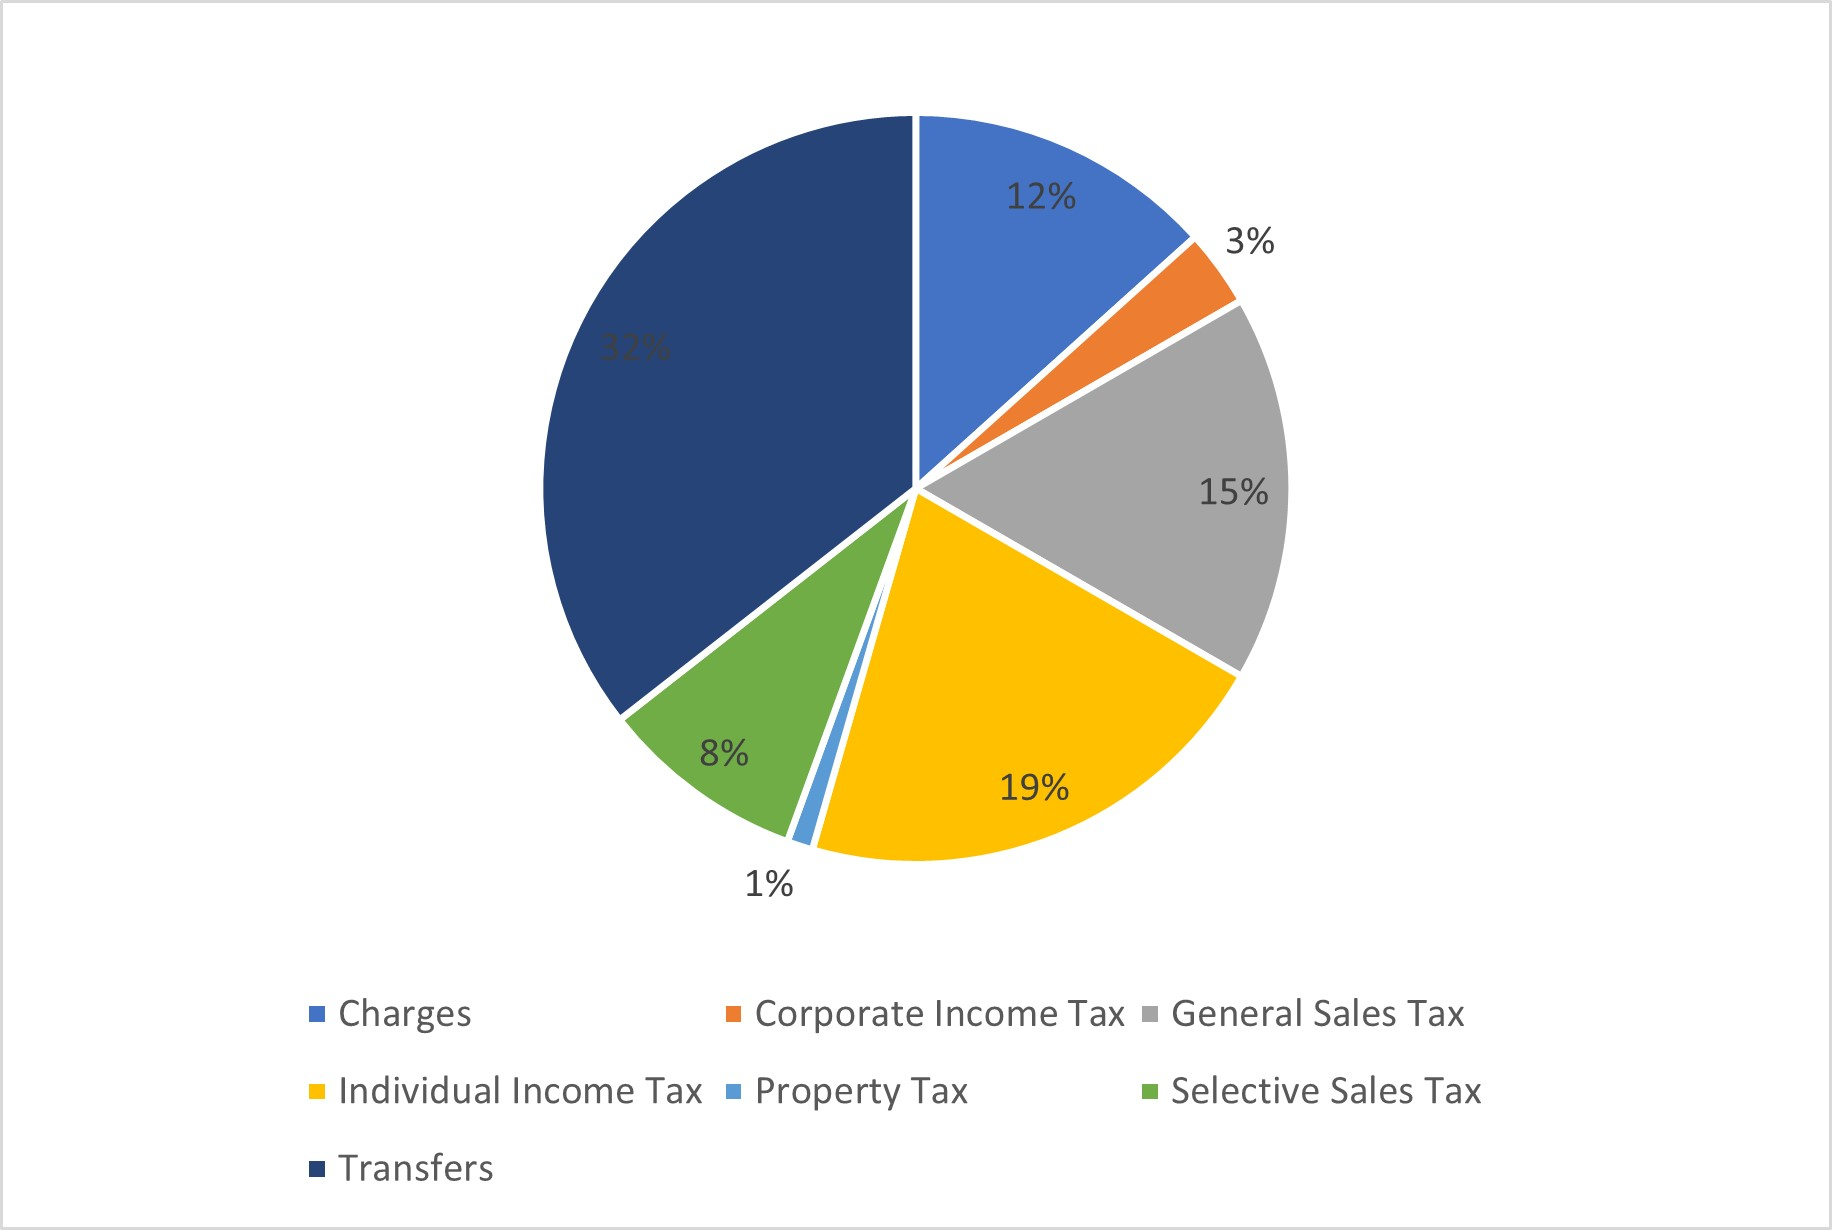
\includegraphics[scale=0.4]{Chapter-1/Figures/source of state general revenue.jpg}%以pic.jpg的0.5倍大小输出
        \end{minipage}
    }
    \subfigure[Source of Local General Revenue]{ %第三张子图
        \begin{minipage}{7cm}
            \centering    %子图居中
            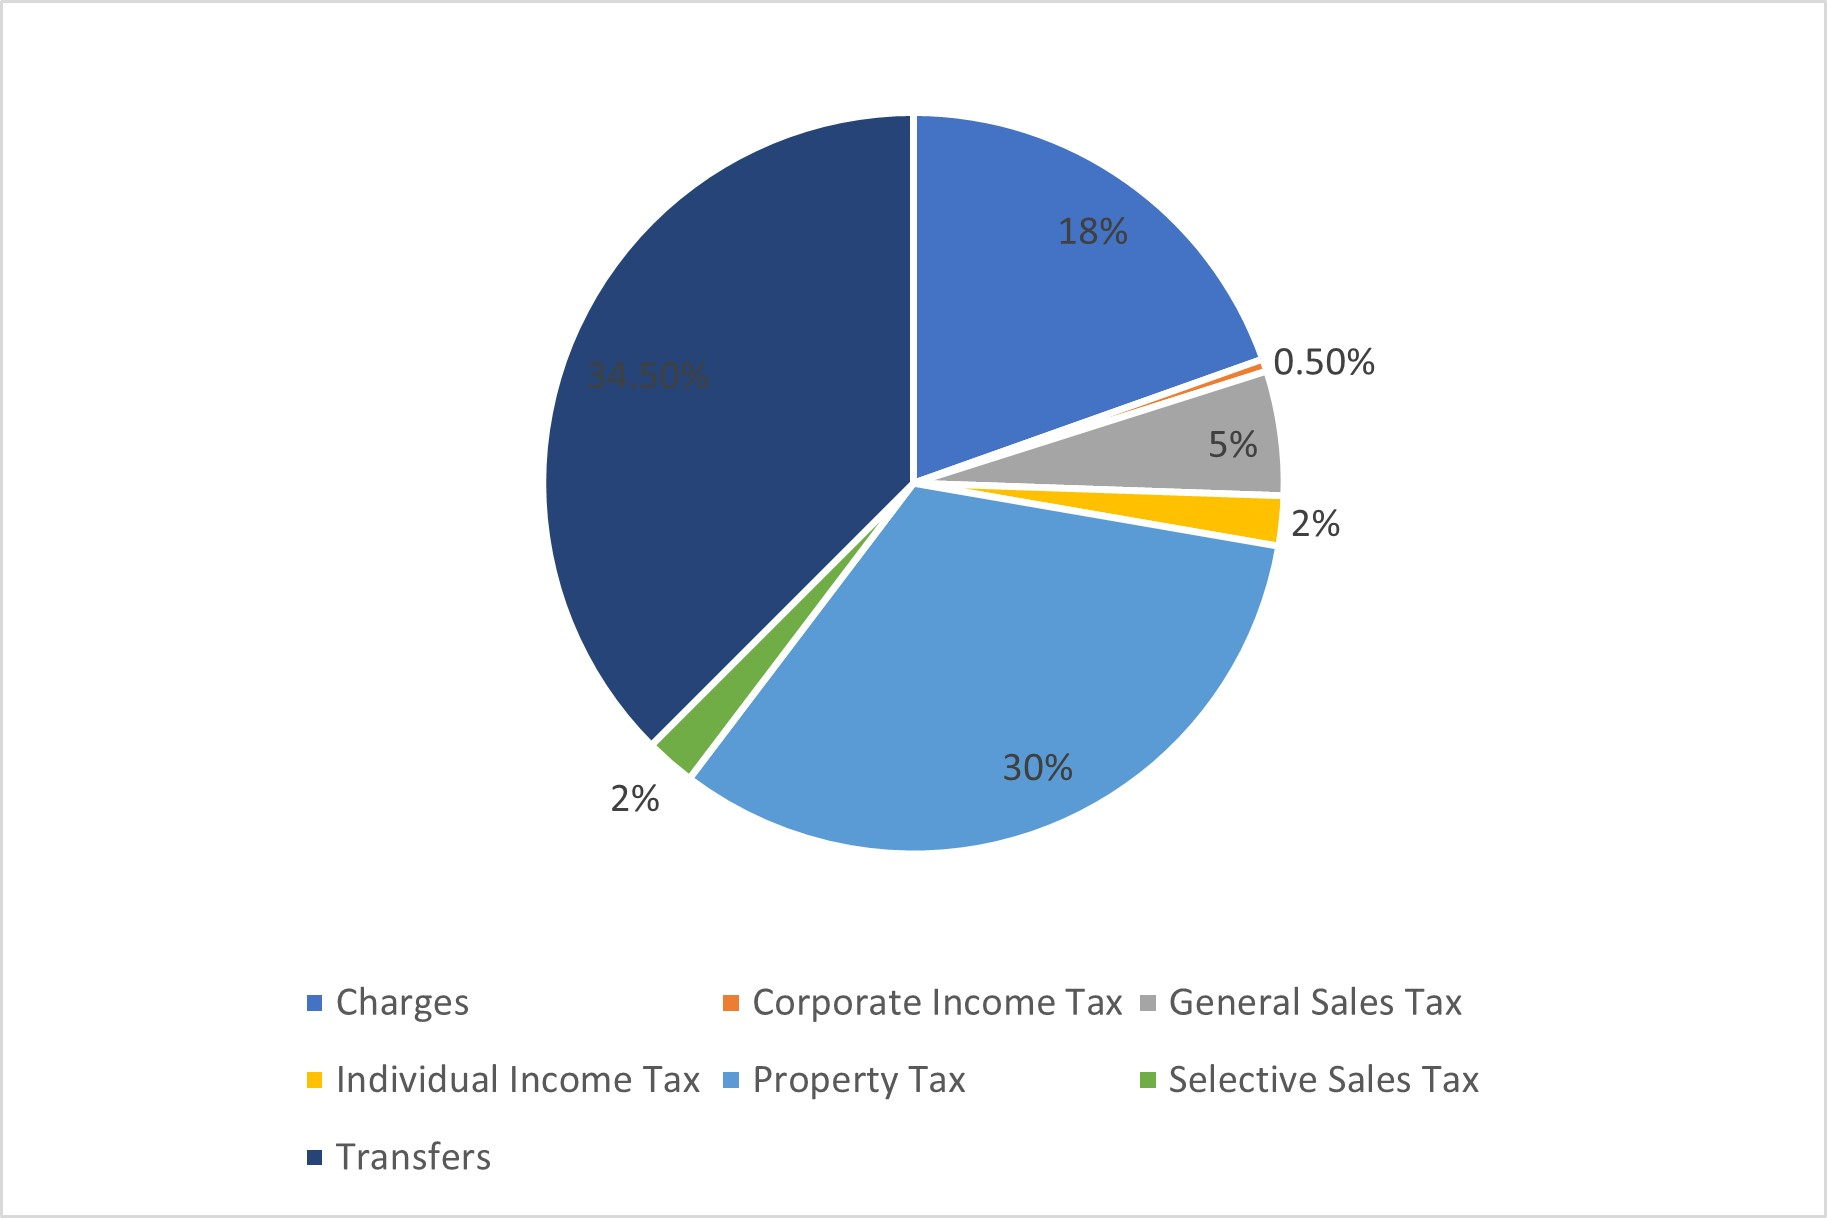
\includegraphics[scale=0.5]{Chapter-1/Figures/sources of local general revenue.jpg}%以pic.jpg的0.5倍大小输出
        \end{minipage}
    }
    \caption[Source of Revenue for Multiple Level of Governments in 2019]{Source of Revenue for Multiple Level of Governments.Data Source:The Department of the Treasury and the Bureau of the Fiscal Service }    %大图名称
    \label{Figure 1.2}    %图片引用标记
\end{figure}
%%%%%%%%%%%%%%%%%%%%%%%%%%    


%%%
%\begin{figure}[htb]
%    \centering
%    \includegraphics[scale=1]{Chapter-1/Figures/Revenue breakdown of United States}
%    \caption[Revenue breakdown of the different levels of governments in 2019.]{Revenue breakdown of the different levels of governments in 2019.
%    \texttt{Source: U.S. Census of Bureau} }
%    \label{Ch1-figure: Revenue breakdown of United States}
%\end{figure}
%%%

On the expenditure side, federal, state and local government functions differently in supplying public goods and services. Filtered out the public-goods-unrelated expenditure such as interest from debt, federal government is paying for income security, social security, health, national defense, highways and infrastructure, medic care, social services such as education, training and employment. Similarly, if filtered out the expenditure which are unrelated to the public goods and services in state and local governments, the left parts include public welfare, elementary and secondary education, higher education, health and hospitals, highways and roads, police, courts, housing and community development.
%%%
%%%%%%%%%%%%%%%%%%%%%%%%%%%%%%%%%%
\begin{figure}[H]
    \centering  %居中
    \subfigure[Federal Expenditure]{   %first subfigure
        \begin{minipage}{7cm}
            \centering    %子图居中
            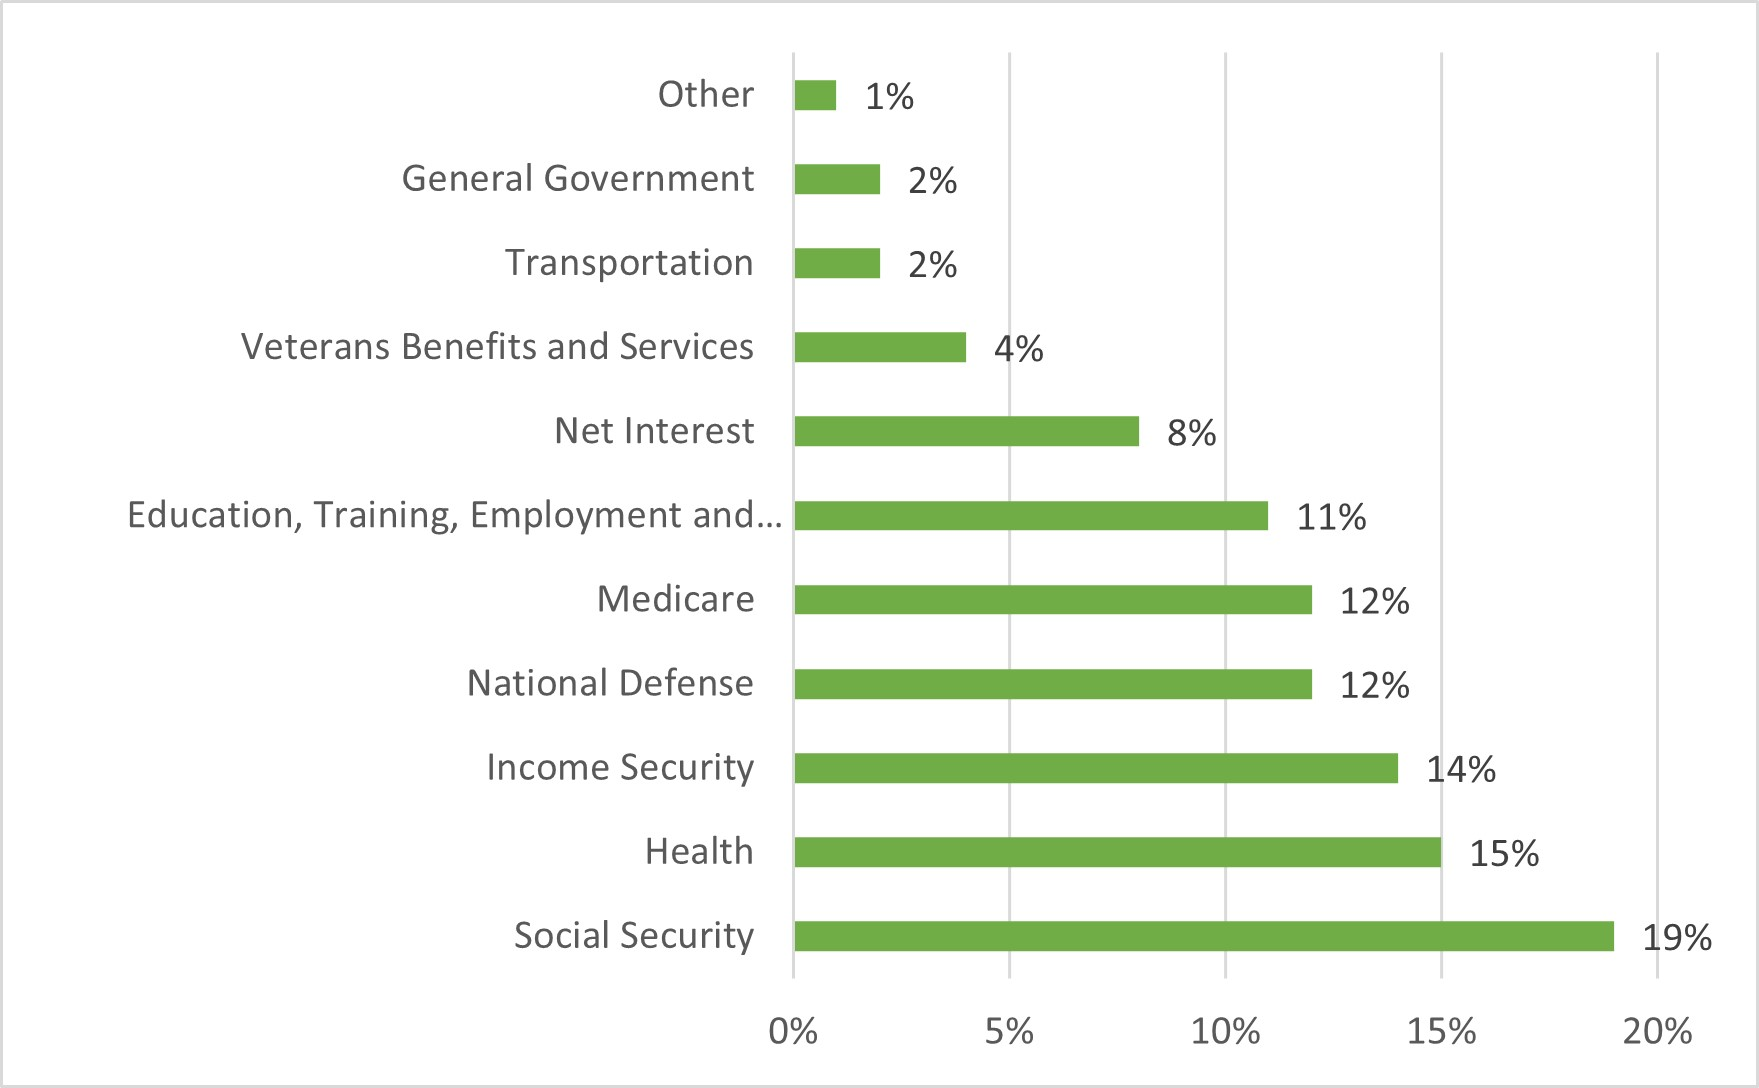
\includegraphics[scale=0.52]{Chapter-1/Figures/federal expenditure.JPG}  %以pic.jpg的0.5倍大小输出
        \end{minipage}
    }
    \subfigure[State and Local Expenditure]{ %second subfigure
        \begin{minipage}{7cm}
            \centering    %子图居中
            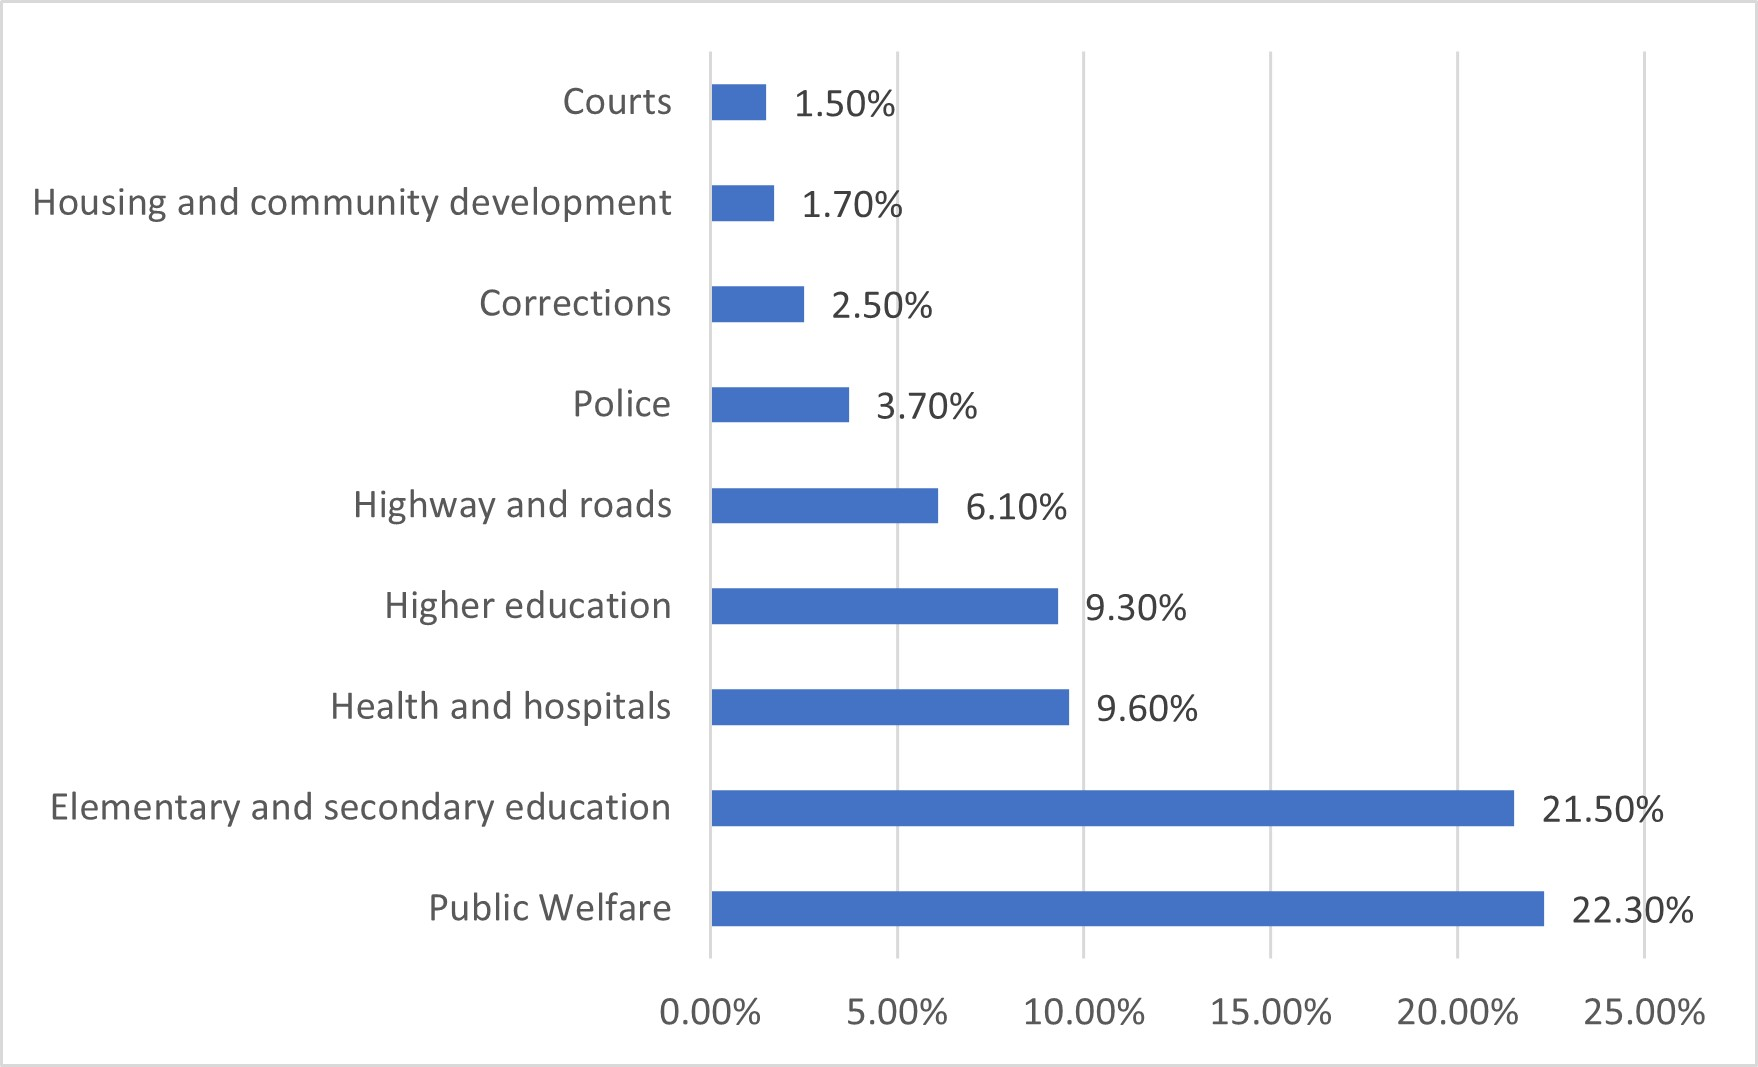
\includegraphics[scale=0.52]{Chapter-1/Figures/state and local expenditure.JPG}%以pic.jpg的0.5倍大小输出
        \end{minipage}
    }

    \caption[Source of Revenue for Multiple Level of Governments in 2019]{Source of Revenue for Multiple Level of Governments.Data Source:The Department of the Treasury and the Bureau of the Fiscal Service }    %caption for whole figure
    \label{Figure 1.3}
\end{figure}

Though The revenue and expenditure structure of federal, state and local government are relatively stable. Figure\ref*{Figure 1.3} shows a cross-sectional data of 2019. A time series fluctuation is presented in Figure\ref*{Figure A.1} attached in Appendix A. Information in Figure\ref*{Figure A.1} shows that it's not a big deal to capture the revenue structure by just breakdown the data in one year.


Federal, state and local government has their unique function in supplying public goods, for example, the federal government is supplying national defense exclusively, while state and local government is the sole supplier in police, courts, housing and community development. Meanwhile, some of the areas are overlapped by both layers of governments, such as public welfare, education, health, highway and infrastructure construction.

\begin{figure}[H]
    \centering
    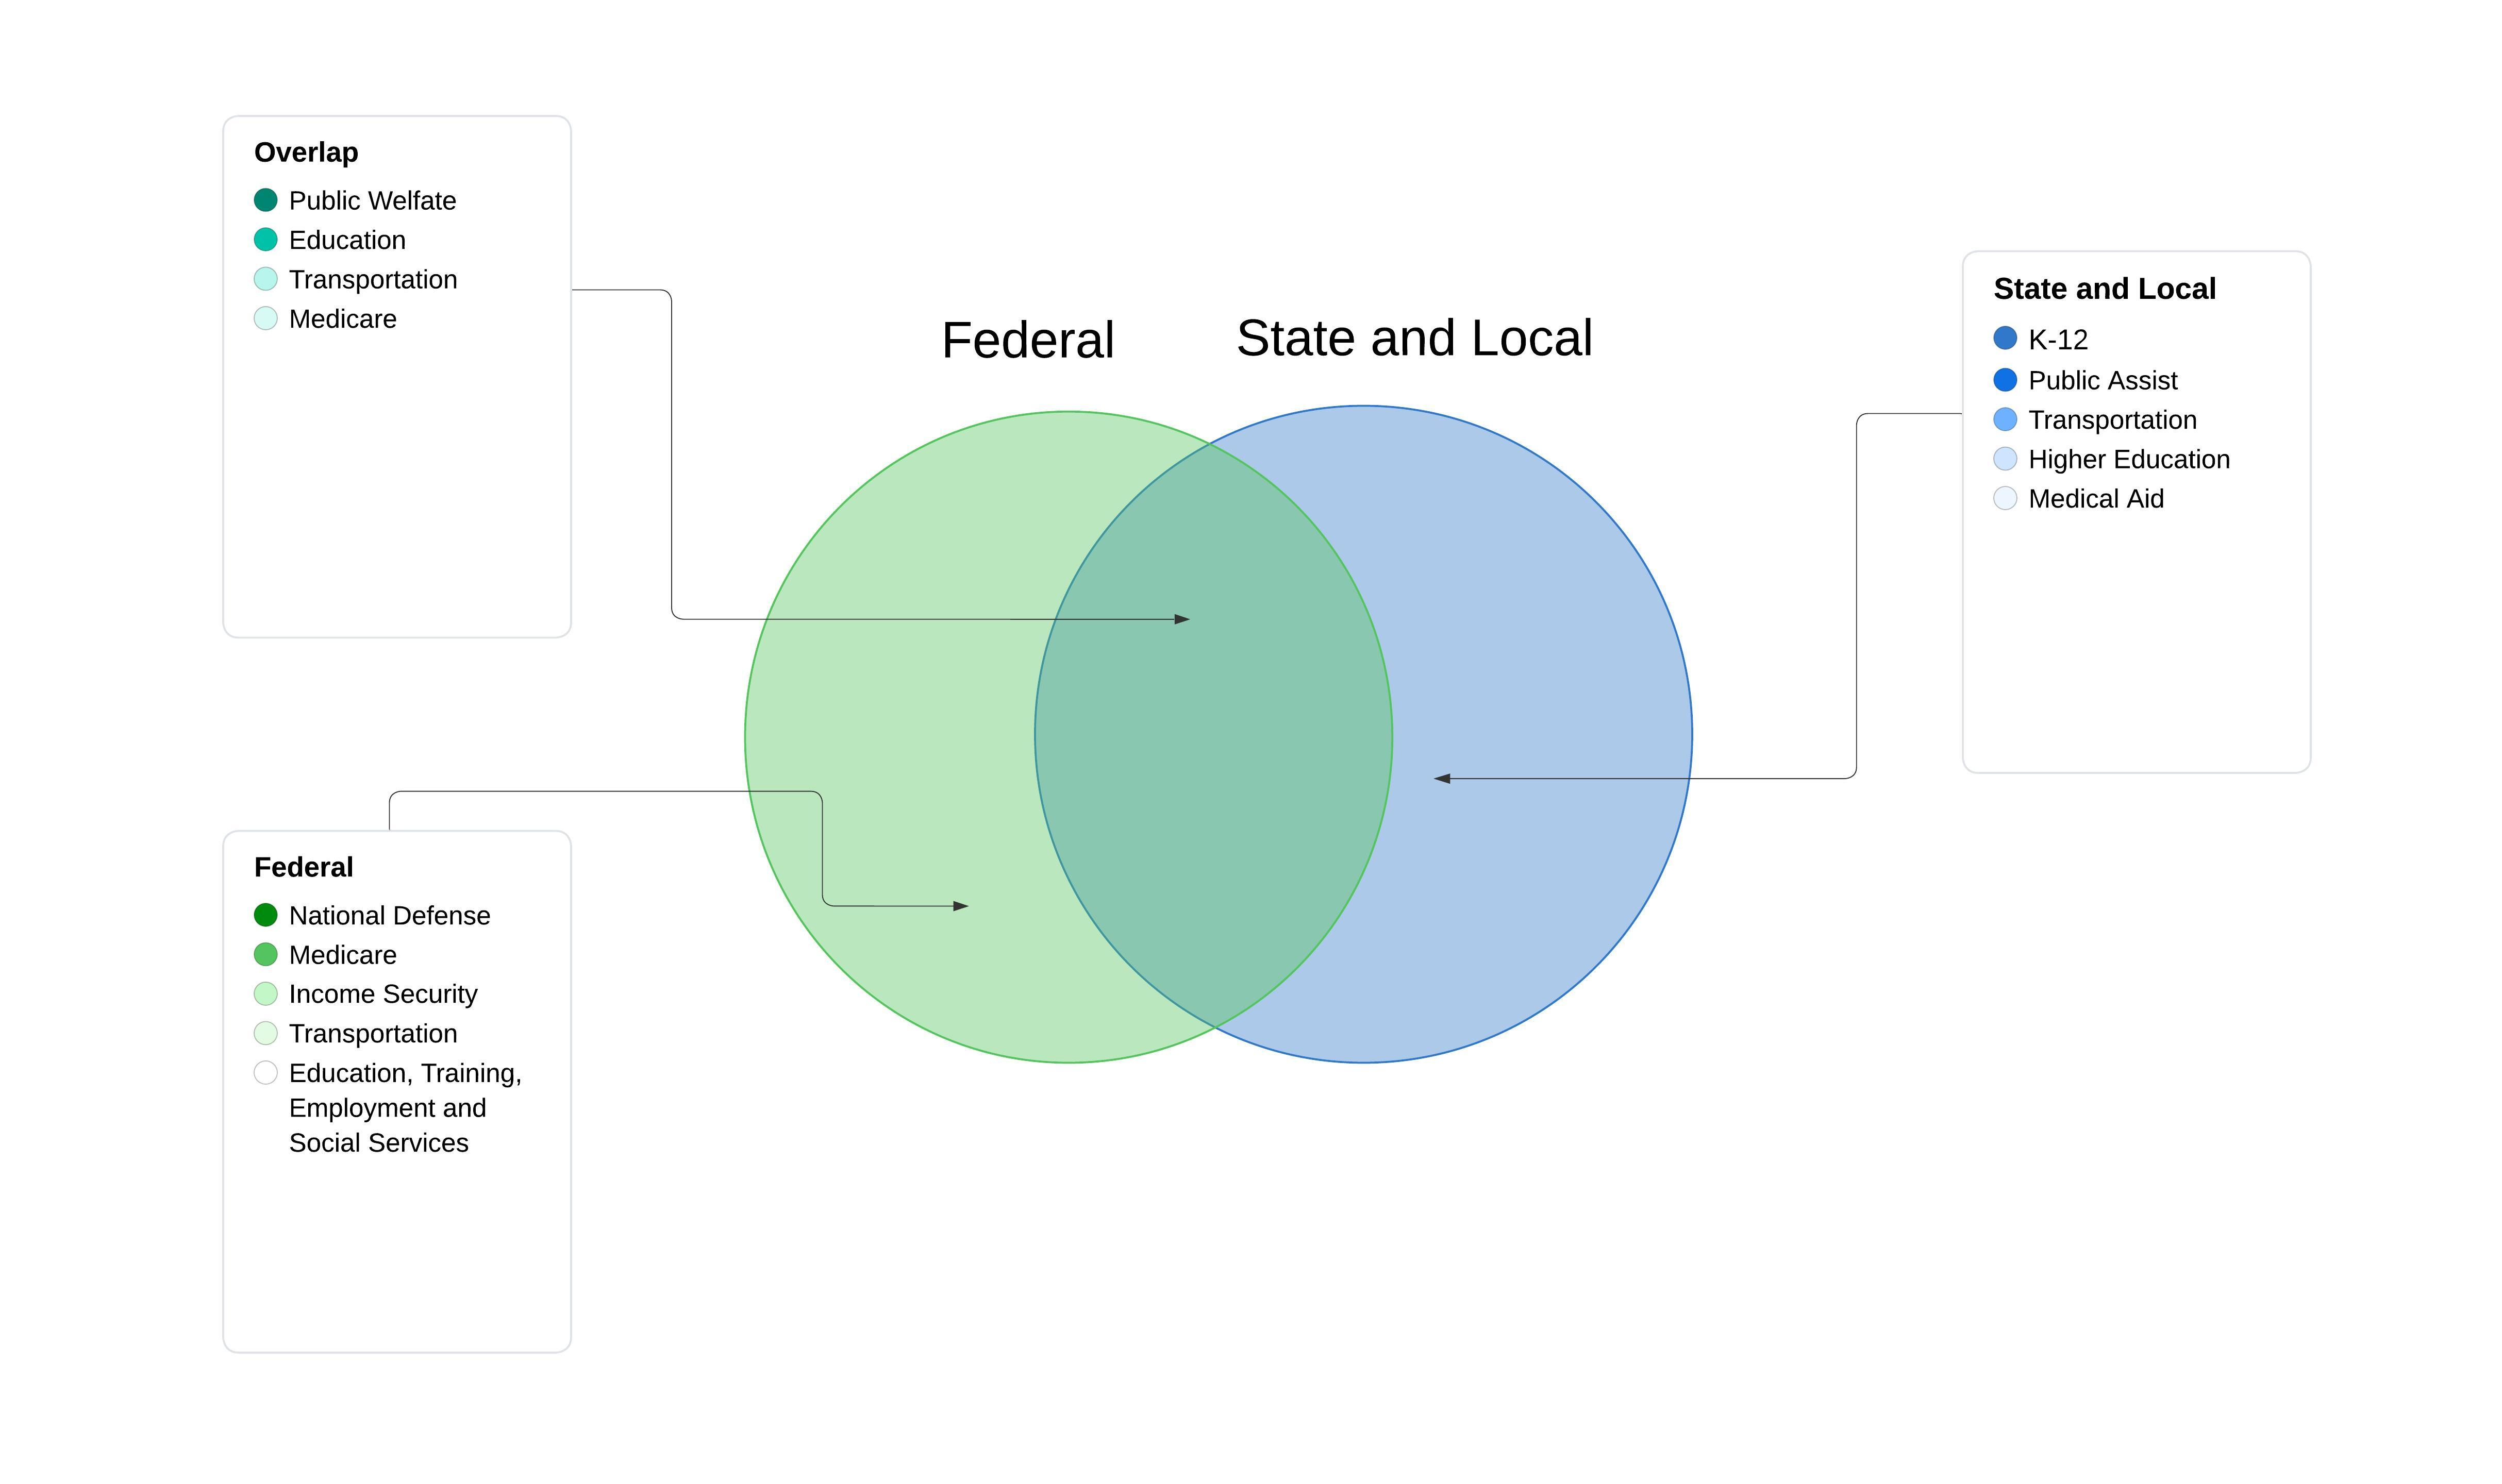
\includegraphics[scale=0.4]{Chapter-1/Figures/Venn graph on public goods.jpeg}
    \caption[Venn graph on public goods and services supplying]{Venn graph on public goods and services supplying by federal, states and local government
        \texttt{} }
    \label{Figure 1.4}
\end{figure}

\subsubsection{Intergovernmental Transfer in America}
In the US fiscal federal system, the Federal government imposes significant influence on state and local fiscal decision making through various grants-in-aids programs (GIA) or intergovernmental transfer(IGT). Annually, these programs amounts to nearly \$700 billion, or close to 20 percent of overall federal revenues \cite{dilger2015federal}. Grounded in fiscal federalism, these programs, are guided by the idea that the allocation of publicly funded goods and services should be the responsibility of state and local governments, due to their closer proximity to the constituents. The sought for advantages of such division include: reduced costs associated with planning and administration, the ability to account for spatial differences, and increased opportunities for citizens to influence political decision-making \cite{musgrave1997devolution}. IGT from federal government help to narrow the gap between revenue and expenditure of state and local government, encourage the supply of specific public goods and promote the horizontal equity among states

%%%%%%%%%%
Generally, grants-in-aids programs in the US federal fiscal system, can be categorized across two dimensions including the level of restrictions that are attached to the awards, and the administrative procedures that govern the award process. In terms of restrictions, GIAs can be organized into categorical grants, block grants and general revenue sharing grants. Categorical grants include formula categorical grants, open-ended reimbursement categorical grants and project categorical grants.Project categorical grants are awarded with relatively strict set of activities that are attached to a specific purpose. Block grants are awarded to fund specific programs, but carry relatively few restrictions. The main difference is that block grants do not attach a specific purpose to how recipients spend the award. General revenue sharing grants carries the least amount of restrictions. In brief, these awards can be spent for any purpose, as long as it is not prohibited by federal or state law.  According to the Congressional Research Service report \cite{dilger2015federal}, there are about 600 grant-in-aid programs, and categorical grants account for about 95 percent of the programs and more than 80 percent of total grant outlays.

% Table generated by Excel2LaTeX from sheet 'Sheet1'
\begin{table}[H]
    \centering
    \caption{Divide Grants by level of Restriction Attached}
    \begin{tabular}{ccc}
        \toprule
        \multicolumn{3}{c}{Level of Restriction}                                   \\
        \midrule
        Low Restriction           & Medium Restriction & High Restriction          \\
        \midrule
        Formula Categorical Grant & Block Grant        & Project Categorical Grant \\
        Open-ended Reimbursement  &                    &                           \\
        General Revenue Sharing   &                    &                           \\
        \bottomrule
    \end{tabular}%
    \label{Table 1.1}%
\end{table}%



In terms of the administrative procedures that govern the awards, the grants can be categorized into three categories including projects grants or competitive grants, formula grants/formula-project grants, and Reimbursement grants. For competitive grants, states should apply by submitting a request and get the grants through a competitive process. They are intended to improve the efficiency of funding allocation by encouraging grantees to seek funds for well-planned and exemplary projects. Formula grants are distributed to states through mathematical formulas decided by social characters within the jurisdiction. Typically the factors in the formula depends on the intention of the grants, and common factors may include population, poverty level, income per capita, unemployment rate, enrollment in public schools, etc. Finally, reimbursement grants awards state and local governments in the form of a reimbursement for a specific percentage of state and local spending on a program.The reimbursement amount does not carry a specific limit. Reimbursement grants could be divided into open and closed ended reimbursement grants. The matching mechanism in reimbursement grants is a very intriguing consideration in public economic literature when evaluating the distortion effect. For matching grants, federal governments will reimburse a specific ratio for each 1 dollar of state and local expenditure. Based on whether federal government set a cap on the matching grants, matching grants can be divided into open-ended matching grants and closed-ended grants.



% Table generated by Excel2LaTeX from sheet 'Sheet2'
\begin{table}[htbp]
    \centering
    \caption{Divide Grants by Form of Administrative Procedure}
    \begin{tabular}{clc}
        \toprule
        \multicolumn{3}{c}{Form of Administrative Procedure}                                                                                                     \\
        \midrule
        \multicolumn{1}{p{9.645em}}{ Submitting Request} & \multicolumn{1}{p{10.285em}}{               By Formula} & \multicolumn{1}{p{10.855em}}{Reimbursement} \\
        \midrule
        \multicolumn{1}{l}{Competitive Grants}           & Formula grants                                          & Project Categorical Grant                   \\
                                                         & Formula-project grants                                  &                                             \\
        \bottomrule
    \end{tabular}%
    \label{Table 1.2}%
\end{table}%




%\subsection{Fiscal Federalism Structure in China}

\subsection{Introduction of the Structure in the Following Chapters}
The goal of this paper is to systematically describe the fiscal federalism structure, explain some of the fiscal phenomenon in the administrative process on the theoretical level using some game theory tool and empirically test the theory I brought up, especially in America. I form the paper by asking and trying to answer a series of questions. The general questions in this research can be divided into theoretical questions and practical questions. Theoretical questions are asking what an ideal framework should be, and practical questions are asking what the actual situation is and I will try to explain the gap between the theoretical design and actual administrative reality. Besides, at least two layers of governments exists in fiscal federalism structure, so by asking theoretical questions and practical questions in two layers of government, I can generate a $2\times2$ table shown in Table \ref*{Table 1.3}.

% Please add the following required packages to your document preamble:
% \usepackage{multirow}
\begin{table}[htb]
    \caption{General Setting of the Questions in Fiscal Federalism Analysis}
    \label{Table 1.3}
    \begin{tabular}{|l|ll|ll}
        \cline{1-3}
        \multirow{2}{*}{}                                                                                                                             & \multicolumn{2}{c|}{Layers of Governments} &                            &     \\ \cline{2-3}
                                                                                                                                                      & \multicolumn{1}{c|}{Central}               & \multicolumn{1}{c|}{Local} &   & \\ \cline{1-3}
        \begin{tabular}[c]{@{}l@{}}Theoretical Questions\\  (ought)\end{tabular}                                                                      &
        \multicolumn{1}{l|}{\begin{tabular}[c]{@{}l@{}}1.What an ideal   fiscal \\ structural should be?\end{tabular}}                                &
        \begin{tabular}[c]{@{}l@{}}2.What is the   optimal reaction\\ for the fiscal policy from central\\ government?\end{tabular}                   &
                                                                                                                                                      &
        \\ \cline{1-3}
        \begin{tabular}[c]{@{}l@{}}Practical   Questions \\ (is)\end{tabular}                                                                         &
        \multicolumn{1}{l|}{\begin{tabular}[c]{@{}l@{}}3. What is the actual decision   \\ making process in the central \\ government?\end{tabular}} &
        \begin{tabular}[c]{@{}l@{}}4.What is the effect of fiscal   \\ policy on local government?\end{tabular}                                       &
                                                                                                                                                      &
        \\ \cline{1-3}
    \end{tabular}
\end{table}


Questions about central government, which are questions on the left side in Table \ref*{Table 1.3} will be investigated in chapter 2, in which I will talk about how to evaluate a revenue and responsibilities combination under a fiscal federalism setting, how a intergovernmental transfer decision is made. Questions about local government on the right side are included in chapter 3, in which I'll talk about the reaction of local government when they receive the intergovernmental transfer. Besides, in chapter 3, I'll try to explain subnational governments' behavior using some game theory tool under the asymmetric setting. In chapter 4, I'll try to find some empirical evidence of the theory inference I generated in chapter 3.







    % !TEX root = ../Yan Hao--Dissertation.tex

\chapter{Questions on the Central Level}
Fiscal federalism is one typical form of fiscal decentralized structure. One consensus among economist and public administrative researchers is that decentralized fiscal structure is obviously more efficient in public goods and services supplying especially in those large and complex country with multiple level of administrative institutions. Hayek \cite{hayek2009use} states that the local government has significant advantages in knowing the information and supply proper kinds and amounts of public goods and services. Hayek's points is the starting points of the research in the advantage of fiscal federalism. Stiliger \cite{stigler1998tenable} followed Hayek's understanding and analyzed the necessity of intermediate and local government especially the necessity of protect the funding ability of those subnational governments. Tiebout \cite{tiebout1956pure} proved theoretically that voting on feat mechanism could promise the matching between public goods supply and needs. Besides, by introducing the competition rule of local governments into public area, Tiebout also proved that the decentralized structure is a promising tool in improving the administrative efficiency. Tiebout's theory seems get supported by the actual data showed in Table \ref*{Table 2.1}, which potentially reflects the difference of tax burden preference of different states. So for the following part, I'll only talk about the evaluation of decentralized fiscal structure, to be more specific, fiscal federalism.


% Table generated by Excel2LaTeX from sheet 'Sheet1'
\begin{table}[H]
    \centering
    \caption{Effective Tax Revenue in America}
    \begin{tabular}{p{9.43em}lll}
        \toprule
        State                & \multicolumn{1}{p{8.145em}}{State and Local Taxes (\$ billions)} & \multicolumn{1}{p{7.43em}}{Personal Income (\$ billions)} & \multicolumn{1}{p{9.93em}}{Effective Tax Rate} \\
        \midrule
        New York             & \multicolumn{1}{c}{177.8}                                        & \multicolumn{1}{c}{1,281.10}                              & \multicolumn{1}{c}{13.90\%}                    \\
        District of Columbia & \multicolumn{1}{c}{7.5}                                          & \multicolumn{1}{c}{55.5}                                  & \multicolumn{1}{c}{13.40\%}                    \\
        North Dakota         & \multicolumn{1}{c}{5}                                            & \multicolumn{1}{c}{39.5}                                  & \multicolumn{1}{c}{12.70\%}                    \\
        Hawaii               & \multicolumn{1}{c}{9.5}                                          & \multicolumn{1}{c}{75.4}                                  & \multicolumn{1}{c}{12.60\%}                    \\
        Vermont              & \multicolumn{1}{c}{3.8}                                          & \multicolumn{1}{c}{32.6}                                  & \multicolumn{1}{c}{11.70\%}                    \\
        \midrule
        United States Total  & \multicolumn{1}{c}{1,652.80}                                     & \multicolumn{1}{c}{16,820.30}                             & \multicolumn{1}{c}{9.80\%}                     \\
        \midrule
        Alabama              & \multicolumn{1}{c}{16.4}                                         & \multicolumn{1}{c}{198.9}                                 & \multicolumn{1}{c}{8.30\%}                     \\
        Oklahoma             & \multicolumn{1}{c}{13.9}                                         & \multicolumn{1}{c}{174.4}                                 & \multicolumn{1}{c}{8.00\%}                     \\
        \midrule
        \multicolumn{4}{p{34.935em}}{\textit{Source:U.S. Census Bureau Dataset}}                                                                                                                             \\
    \end{tabular}%
    \label{Table 2.1}%
\end{table}%


\section{How to Evaluate the Fiscal Federalism System}
Even within the topic of fiscal federalism, the fiscal federalism structures in different countries have different content and features, needless to say, they show different impact in public goods and services supplying. Like I mentioned in Chapter 1, it's hard and nearly impossible to find a perfect stick yard criterion to compare fiscal federalism in different countries. I'll try to explain and get a comprehensive way to evaluate fiscal federalism. Literature about fiscal federalism can be roughly divided into two groups. First-generation theory of fiscal federalism concentrate on the fiscal structure itself, focusing on the efficiency of federalism in collecting revenue and offering responsibilities, and whether the revenue-responsibility combination perform well in public goods supply. Coming to second-generation theory of fiscal federalism, scholars get interested in the effect of fiscal federalism on other area such as the effect on economic development.

\subsection{First-Generation Theory of Fiscal Federalism}


One popular aspect to estimate if the  fiscal structure is reasonable is to evaluate the fiscal structure economically. In another word, to estimate if the combination of funding and responsibilities meet Pareto efficiency, which happens when resources are so allocated that it is not possible to make anyone better off without making someone else worse off \cite{pareto2014manual}. This is also the most common understanding wildly accepted by both economic and public administrative researcher.  Under economic view, three directions are helpful in estimating the fiscal structure, including externality, information complexity and incentive compatibility. Firstly, about externality, an ideal setting is to initialize the externality as much as possible for both positive and negative externality.Oates' \cite{oates1972fiscal} work on fiscal federalism is a milestone for modern fiscal federalism research, one principle he mentioned in his work is that government and the residents living in the jurisdiction should pay for their negative externality and get paid for positive externality.Olson \cite{olson1993dictatorship} states that the "free rider" issue could be overcome by making the jurisdiction and the  beneficiary area identical, besides, the equilibrium under this setting could make marginal cost equal to marginal benefits. The externality evaluation is obviously an efficiency consideration. One example of efficiency consideration in America's fiscal federalism setting is the revenue structure related to individual tax. As is shown in Table \ref*{Table 2.2}, for the tax object that are convenient to move freely,such as individuals,individual income tax is mainly collected by federal governments and state governments to minimize the behavior distortion and improve efficiency.Since in that way, individuals are indifferent to where they live and where to pay their tax.

% Table generated by Excel2LaTeX from sheet 'Sheet1'
\begin{table}[htbp]
    \centering
    \caption{. Percentage Composition of Tax Revenue by Government Level}
    \begin{tabular}{lccc}
        \toprule
        \multicolumn{1}{c}{Type} & Federal & State   & Local   \\
        \midrule
        Individual income        & 51.80\% & 37.20\% & 4.70\%  \\
        Corporate income         & 6.90\%  & 4.70\%  & 1.10\%  \\
        Other taxes              & 41.20\% & 58.10\% & 94.20\% \\
        \bottomrule
    \end{tabular}%
    \label{Table 2.2}%
\end{table}%


Secondly, information complexity in administration process is also a important consideration in evaluating the fiscal federalism structure. Except for the earlier job represented by Hayek and Tiebout, Bsley et al \cite{2003Centralized} set up a political economy model to simulate the decision making process in a democratic country, in their model they introduced insensitivity of central government into their model and emphasized the advantage of local government in public goods supplying. Besides, the information communication is mutual. For one,local governments know local residents' needs better, besides, local governments' behavior could be better perceived by local residents. Dethier \cite{martinez2003fiscal} mentioned that the decentralized structure of fiscal federalism put the local government under supervision. Based on Dethier's idea and Tiebout's voting on feet framework, Baicker \cite{baicker2005spillover} set up a horizontal competition structure, he introduced multiple local governments and states that under yardstick competition framework, decentralized fiscal structure will help local residents get a direct evaluation about  local governments' efficiency in public goods supply, thus help them easier to "vote on feet". Local governments should get pushed by this information transparency.

Finally, a good fiscal structure should have incentive compatibility. Incentive compatibility is a game theory analysis tool introduced by Leonid Hurwicz \cite{hurwicz1973design} wildly used by business management area at first. A mechanism is called incentive-compatible (IC) if every participant can achieve the best outcome to themselves just by acting according to their true preferences. Incentive compatibility was introduced into public administration and public economics area and became an important criterion to evaluate the quality of fiscal federalism. Local governments could be motivated to supply proper amount and quantity public goods with efficiency under proper fiscal federalism setting. Eckstein \cite{eckstein1958water} points out that the proper combination between funding resource and responsibilities could be a great motivation for any kinds of organizations. Under Eckstin's setting, at least in democratic country, working hard with efficiency in public goods supplying is an weakly dominate strategy since that will attract more residents and increase more public funding resource. Another clue is that for most of the scholars, when they  investigate the related topic and talk about governmental fiscal behavior, while the central government's goal is hard to define, by default they just assume the local government's target is to maximize the local fiscal revenue(Baretti, Bucovetsky,Dahlby,Jha) \cite{baretti2002tax,bucovetsky2006efficiency,dahlby2011marginal,jha2000tax}.

The main theme of the first-generation theory of fiscal federalism is to approve the positive effect of this decentralized structure, confirm the positive effect in public goods supplying. The main investigation is to evaluate the role of fiscal federalism in the public goods efficiency. Most of literature in this period is theoretical investigation.

\subsection{Second-Generation Theory of Fiscal Federalism}
When it comes to the second-generation theories, scholars do not merely stare at the efficiency of fiscal federalism in public goods supplying. For further step, they start to notice the relationship between fiscal federalism and other social area, such as economic development \cite{cai2005does,barro1991economic}, local government behavior \cite{jin2005regional}, etc. One obvious change is that, second-generation theory researchers, though still admit the fundamental effect that fiscal federalism played in public goods supply, start to emphasize that fiscal federalism may not always works perfectly especially in developing countries \cite{keen1997fiscal,treisman2002decentralization,bardhan2002decentralization,bucovetsky2005public}. I summarized the second-generation fiscal federalism literature and divide all these literatures into three categories, which are relationships with economic development, political intention, and effect on local governmental fiscal behavior.

The investigation about the relationship between fiscal federalism and economic development also inspired by Charls Tiebout \cite{tiebout1956pure}. Though Tiebout's theory has been supported by huge amounts of econometric evidence, his theory is obviously inspired by American fiscal structure. Most of the assumptions in Tiebout's setting are hard to achieve especially in developing countries. Since Tiebout just assume local governments have the ability to supply public goods with proper efficiency. Based on that assumption, he answered how to match the preference from the residents with the ability of the local government. Some second-generation theory literatures tried to open the black-box in Tiebout's assumptions. Some researchers noticed the role of production factors in fiscal federalism setting. A lot of econometric evidence that even in developed countries such as european union, the residents within one country are not moving totally freely, needless to say the movement across different countries \cite{oates2004essay}. Even for the residents who moved across different jurisdiction, the performance in public goods supply is not their main concern according to Faguet's servey \cite{faguet2004does}. Except for the population movement, capital is also a interesting factor in fiscal federalism. Mckinnon \cite{mckinnon1993order} attribute the economic boost in southern United States to the low factor cost including capital, labor and land. He then did a follow up research claims that the compensation and equalization effect of transfer payment in fiscal federalism system may block the flow of production factors. Cai and Treisman \cite{cai2005does} proved that with initial difference in resource endowment, the decentralized feature of fiscal federalism may lead to local governments' sturdiness in economic development since the moving of capital seems surely lead to development imbalance, the imbalance between different jurisdictions will destroy the enthusiasm of local governments. Based on research related to resource endowment imbalance, Treisman \cite{treisman2002decentralization} took one step further, he emphasized that local government of the jurisdiction with low resource endowment tend to spend more on decreasing poverty instead of the target related to economic development efficiency.

Second-generation theory scholars noticed the effect of fiscal federalism on local governmental behavior, such as the effect of intergovernmental transfer on local governmental's tax collecting effort \cite{mogues2012external}, the effect of intergovernmental transfer on local governments' spending structure \cite{hines1995anomalies}, relationship between fiscal federalism and local government debt \cite{qian1998federalism} etc. The effect of fiscal federalism on local governmental's behavior will be analyzed in the asymmetric setting in Chapter 3.

Except for merely economic consideration, another consideration is political intention. Though not so popular, political factor explains a lot of fiscal federalism design that can hardly be explained by economic and efficiency theory. Fiscal federalism in Canada plays an important role in equalization across different jurisdiction, thus this fiscal system is like the glue for the political federalism, similar econometric evidence can be found in Australia  \cite{oates2005toward}. However, the fiscal federalism in Italy shows a different look, the transfer payment mechanism from high fiscal revenue area to low revenue area exacerbate the conflict between different jurisdiction.

\begin{figure}[htb]
    \centering
    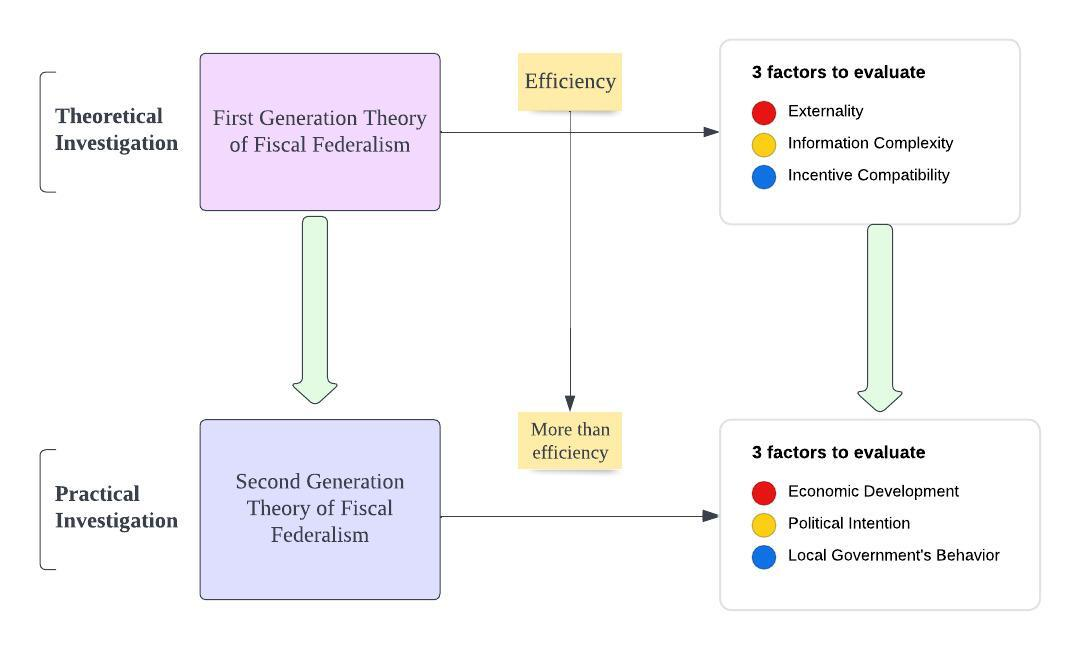
\includegraphics[scale=1]{Chapter-2/Figures/how to evaluate the fiscal federalism.jpeg}
    \caption[How to evaluate the fiscal federalism]{How to evaluate the fiscal federalism
        \texttt{} }
    \label{Figure 2.1}
\end{figure}


To summarize, as is shown in Figure \ref*{Figure 2.1}, initial research about fiscal federalism designed a theoretical ideal framework to supply public goods efficiently. In developed countries especially in America, scholars did find some empirical evidence to support the benefits of this decentralized fiscal structure. However in developing countries, the fiscal federalism didn't work out perfectly, this administrative fact inspired the second-generation theory, scholars starts to focus on the other side of the coin.

Except for the combination of revenue and responsibilities within each jurisdiction, the interaction between governments is also an intriguing topic for fiscal federalism researchers. The interaction between governments can be divided into horizontal interaction which means the interaction among same level, and vertical interaction which means interaction between central and subnational governments. I'll focus on the vertical interaction in this paper.

\section{How Intergovernmental Transfer Decision is Actually Made}

\subsection{Game Theory Modeling of Bargaining Process}
In America, every year nearly \$700 billion, or nearly 20 percent of overall federal revenues, are allocated toward various state and local government grant programs. The mechanism of intergovernmental transfer distribution has always been an intriguing topic in the public finance area.

The grants distribution decision in democratic countries is viewed as an bargaining game within a specific decision-making group, such as a specific committee, the congress or the house,depends on which group is the decisive institution. For the bargaining models to simulate the grants distribution bargaining, four assumptions are quite important among all the necessary assumptions: recognition rule, voting rule, amendment rule and money-distribution rule. Recognition rule means how to decide who to make the proposal. In another word, the rule to choose an agenda setter.for example most of the literature assume the random recognition rule \cite{kalandrakis2004three,anesi2015bargaining,diermeier2011legislative,rosenstiel2021congressional}, which means $n$ members among the decision making institution have equal probabilities to be chosen to make the initial proposal. Voting rule means the standard to judge if the proposal is passed,common voting rule include majority rule and unanimously voting rule. Amendment rule means the constraints on making amendments,ranging from the closed rule, in which no amendments are allowed, to the open rule, in which any and all (germane) amendments are allowed. Grants-type rule means how grants could be manipulated by decision making institution, for example, some scholars assume the decision making institution can directly decide the number among the receivers, which is referred as "earmarks" or "pork barrel" spending model.

Baron and Ferejohn \cite{baron1989bargaining} is the fundamental work for all the following bargaining model analysis. They assume random recognition, majority voting rule and earmarks rule. Baron and Ferejohn \cite{baron1989bargaining} and the generalization of their work by Banks and Duggan\cite{banks2006general} show that legislators with proposal or agenda-setting power receive a disproportionate share of funding. Another feature of the equilibrium is that funds only go to legislators that vote for the proposal which is the winning coalition, with zero dollar goes outside of the winning coalition. Besides, according to their inference, when the proposal are brought up under closed rule, the winning coalition is minimal, which means members of the winning coalition maximize their benefits.

Though pioneering in this field, in actual political environment,bare amounts of grants are similar to "earmarks", the earmarks assumptions heavily restrict the explanatory power in grants distribution. Martin \cite{martin2018dividing} extends Baron and Ferejohn's model by loosen the earmark assumption. He restrains the power of members in decision making institution by only allowing them to decide the factor of the formula, not decide the number arbitrarily. As mentioned in Chapter 1, this modification in assumption is a big step to the actual political and administration life. Martin gets some different conclusions compared to Baron and Ferejohn, unlike Baron and Ferejohn’s model, Martin predicts an oversized winning coalitions, and emergence of persistent winning blocs. Besides, he proved that when bargaining over a low-dimensional formula (i.e., a formula based on a small number of state characteristics), legislators have relatively little latitude in targeting funds to specific districts, this prediction is supported by some empirical evidence, Martin studied all the existing formula grants and count the number of the factors in the formula, he points out that 95\% of the formula have less than 5 variables, which means members have less than 5 dimensions to bargain about, the ability to manipulate the formula is highly limited. Since members can only decide the factors among the formula, inevitably, some jurisdiction with similar features can be a free riders, even if the free riders do not belong to winning coalition, thus Martin predicts positive distribution outside the winning coalition.

\subsection{Some Empirical Evidence for the Grants Distribution}
Except for the general introduction related with intergovernmental transfer in Chapter 1, a challenge with the distribution of IGT is that they take place in a political environments, where individual political agendas have the potential to influence the outcome of IGT allocations in ways that are inconsistent with the intended structure of the distribution procedures.Based on some classic game theory analysis within the congress. Given the important role of GIA in the US federal system, the influence of politics on the allocation of IGT often comes at a high cost. There is plenty of anecdotal examples that illustrates the potential costs, including Robert Carlyle Byrd's spending two decades of his career directing as much federal spending as possible to his home state, saying he wanted to be "West Virginia's billion-dollar industry".

In Markusen, Saxenian and Weiss's \cite{markusen1981benefits} descriptive study, they define three distinctive swings in the distribution of federal grants to cities in the 1960s and 1970s during which federal grants grew by a tremendous amount and northeastern and midwestern cities benefit most from 1965-1972, southern and western cities benefits most from 1972-1975, and a slight swing back in favor of the first group from 1975-1978. One possible inference in their article is that the political background may partially explained this swings. Stegarescu \cite{stegarescu2006decentralised} explains that the degree of IGT decentralization is a result of population, unemployment, trade-openness, presidential regimes and electoral systems based on the test result of the panel data of 17 nations. Kasdin \cite{kasdin2016decision} does an empirical test and mentions that state or local government governmental network complexity is a factor influencing federal transfer amount and federal controlling extent. He finds that higher-level government tends to relinquish some control when lower governmental network is highly complicated, but the amount of the transfer is negatively related with the complexity. One possible relationship behind this relationship is that high complexity is a barrier hinder politicians to claim the political credit, thus they are less motivated to secure the fiscal revenue for their representative jurisdiction. Larcinese, Rizzo, Testa \cite{larcinese2006allocating} tested the impact of the president on the amount of federal transfer to state government. They find that state that heavily supported the incumbent president in past presidential elections tend to receive more funds. Wallis \cite{wallis1987employment} also emphasizes the political effect on the amount of intergovernmental transfer. He claims that states with the high volatility of presidential vote receive significantly more federal support based on his study on the longitudinal data of all states in the U.S. Markusen, Saxenian and Weiss \cite{markusen1981benefits} defined the supply side and demand side when investigating the mechanism of the IGTs decision-making process, even though they don’t point out the specific factors, they emphasize that the IGTs is the result of the political, economic and social characteristics of both demand and supply side.

All these literature seems imply the political factor even some biased factor impact the intergovernmental transfer. To summarize the literature listed above, one implication is that the factor that impact the intergovernmental transfer comes from not only from the legislative decision-making institution, also from administrative branch. Another implication is that political stance of local jurisdiction seems influential in intergovernmental distribution.

\section{An Empirical Investigation on IGT Distribution Mechanism}
Combined with Martin's \cite{martin2018dividing} conclusion introduced in section 2.2.1 and all the literature implying the political impact mentioned above, I design and conduct an longitudinal empirical test to statistically investigate the intergovernmental transfer mechanism. Specifically, I try to solve two questions in this empirical design, for one, following Martin's inference, how much extent does states share similar characteristics so the IGT benefits goes outside of the winning coalition. Another questions I wander is, following Markusen, Saxenian and Weiss's framework, if we got the social and economic characteristics control, how much can political factors affect the IGT. The reason I focus on the political factors is that, contradictory to what we discussed in section 2.1, the political factor seems unrelated to efficiency, thus may cause more distortion and waste of resources. Besides, examination on political factors could be important because of the sharp rise in hostility between democratic and republican parties. The potential effects of political party control may impact the IGT grants distribution significantly.

\subsection{Sample and Characteristic Selection}
I focus on the direct IGT from federal government to state governments in America. To incorporate the political impact into the data framework, I did a stratified sampling to collect states sample from traditional republican states, traditional democratic states and swing states.
The state grouping method are based on two criterion, the historical presidential election result and the winning rate following Beachler,Donald,Bergbower,Matthew etc.'s work \cite{beachler2015presidential}. The democratic states and republican states are those chose same party in the president election since 1984 with wining rate over 58\%. The swing states are those have chosen president from two parties and the winning rates are less than 58\%.

The states collected into my sample can be listed as Table \ref*{Table 2.3}

% Table generated by Excel2LaTeX from sheet 'Sheet1'
\begin{table}[H]
    \centering
    \caption{States Sample and Grouping}
    \begin{tabular}{p{7.57em}cc}
        \toprule
        States         & \multicolumn{1}{p{7.93em}}{Group}                    & \multicolumn{1}{p{6.855em}}{Code} \\
        \midrule
        Wyoming        & \multicolumn{1}{c}{\multirow{5}[2]{*}{Red States}}   & \multirow{5}[2]{*}{1}             \\
        Idaho          &                                                      &                                   \\
        Kansas         &                                                      &                                   \\
        Nebraska       &                                                      &                                   \\
        North Dakota   &                                                      &                                   \\
        \midrule
        Maryland       & \multicolumn{1}{c}{\multirow{5}[2]{*}{Blue States}}  & \multirow{5}[2]{*}{2}             \\
        Massachusetts  &                                                      &                                   \\
        Rhode Island   &                                                      &                                   \\
        New York State &                                                      &                                   \\
        Washington     &                                                      &                                   \\
        \midrule
        Pennsylvania   & \multicolumn{1}{c}{\multirow{4}[2]{*}{Swing States}} & \multirow{4}[2]{*}{3}             \\
        Nevada         &                                                      &                                   \\
        Wisconsin      &                                                      &                                   \\
        Ohio           &                                                      &                                   \\
        \bottomrule
    \end{tabular}%
    \label{Table 2.3}%
\end{table}%

The social and economic characteristics that commonly included in the formula when doing the intergovernmental transfer are population, working age population weight, median household income, unemployment rate, road mileage and gdp \cite{dilger2015federal}. I collected all factors mentioned in Dilger's service\cite{dilger2015federal} of the sample states, besides, I also take reference from some major intergovernmental transfer programs such as Medicaid, the Title I-A education program, Temporary Assistance for Needy Families (TANF), Section 8 Housing Choice Vouchers, and the Community Development Block Grant (CDBG) to collect factors comprehensively. I also did proper operation for data regression convenience and better data visualization. The characteristics I collected and source of data can be listed as Table \ref*{Table 2.4}.

\begin{table}[H]
    \centering
    \caption{Social characteristics for Sample States}
    \begin{tabular}{cp{6.43em}p{9.285em}p{5.855em}p{5.355em}}
        \toprule
        \multicolumn{1}{p{4em}}{Variables } & Definition                      & Operation          & Source                              & Time Period                  \\
        \midrule
        gdp                                 & \multicolumn{1}{c}{Real GDP}    & Log transformation & FRED                                & 2000-2019 annually collected \\
        \midrule
        lgp                                 & \multicolumn{1}{c}{Population } & Log transformation & Census of bureau                    & 2000-2019 annually collected \\
        \midrule
        wapw                                & Working age population weight   & No operation       & Census of bureau                    & 2000-2019 annually collected \\
        \midrule
        mhi                                 & State median household income   & Log transformation & Census of bureau                    & 2000-2019 annually collected \\
        \midrule
        ur                                  & unemployment rate               & No operation       & FRED                                & 2000-2019 annually collected \\
        \midrule
        prm                                 & public road mileage             & Log transformation & Bureau of transportation statistics & 2000-2019 annually collected \\
        \bottomrule
    \end{tabular}%
    \label{Table 2.4}%
\end{table}%


\subsection{Principle Components Analysis of Social and Economic Characteristics}
%%principle components analysis
%%%%%%%%%%%%%%%%%%%%%%%%%%%%%%%%%%%%%%%%%%%%%%%%%%%%%%
As mentioned above, too many factors may exists in the formula that decides the grants distribution. What's even worse, one can distinguish the multicollinearity problem in the variables I collected just by intuition, for example, working age population weight and unemployment rate are strongly related variables, higher population is doomed to occupy more public road. To answer the first question,these two problems are obvious hinder thus it's hard to judge how similar jurisdictions could be in social and economic characteristics directly. So I conduct a primary components analysis to reduce the data dimension and overcome multicollinearity problem to check if the reduced-dimension data are cluster distributed or scattered distributed.

According to the primary components variance analysis result, the explained variance of each primary components ration is $ [9.26107325e-01 6.46212361e-02 8.18645817e-03 1.03638367e-03
            4.62668749e-05 2.33064549e-06]$, the first two dimension 97.5\% of the information, thus I only keep the first two dimensions. By only keeping the two principle components with most information, comparing the characteristics between jurisdictions became a possible procedure. The scatter plot after data dimension reduction is shown as Figure \ref*{Figure 2.2}

\begin{figure}[H]
    \centering
    \includegraphics[scale=1]{Chapter-2/Figures/pca.png}
    \caption[Social Characteristics Principle components Analysis]{Social Characteristics Principle Component Analysis
        \texttt{} }
    \label{Figure 2.2}
\end{figure}

Though reduced dimensions do not have specific economic meaning, but one clear information shown in Figure \ref*{Figure 2.2} is that a lot of states characteristics are cluster distributed, which means plenty jurisdiction features in my data are quite are quite similar. This implication is a side evidence for Martin's \cite{martin2018dividing} deduction that some jurisdiction with similar features can be a free riders, this also predicts the funds outflow of the winning coalition.

Another potential implication is that, the distribution is obviously hierarchical  in terms political parties. Republican states, republican states and swing states are clearly cluster distributed in their own area. Red dots and blue dots distributes on two sides while swing states in the middle. This means any modification on the grants formula that benefits one party is a huge damage to another. This may explain why in the legislative bargaining process, two parties are sharply opposed and swing states are relatively indifferent. This is not counterintuitive, since traditional republican states are highly likely to share similar social characteristics, but this figure may offer a different view on any fiscal collective behavior of the party. When a member in the bargaining process take any behavior, are they doing that due to their political status or arguing benefits for their represented jurisdiction? It seems that any collective political behavior within a party should find a micro-foundation. In other words, when analyze the motivation,one should focus on the motivation of particular member rather than the benefits that a group can take.

\subsection{Political Impact Investigation}
%%political factor regression
%%%%%%%%%%%%%%%%%%%%%%%%%%%%%%%%%%

The goal of this section is to  develope and test a theoretical framework that seeks to further advance the understanding of how the above factor outside of the bargaining institution can affect the spatial distribution of IGT. I still focus on the intergovernmental transfer from federal to state governments. Toward this end, based on the literature implication I collected in section 2.2.1 and 2.2.2, I explore how combination of political party control across legislative and administrative branches affects the distribution of IGT. The factor I'm interested includes whether legislative and administrative branches is unified, whether Democratic or Republican party has different preferences, and whether party control is aligned across the federal and state governments. The distribution of IGT is affected by (1) political party distribution across the federal and state government, and by (2) political party affiliation (i.e., Republican or Democratic party). I also examine how the perceived importance of a state in the federal political process affects the distribution of IGT. In addition, to gain insight into the role of swing state,I also examine the relationship between the IGT and whether a particular state is considered a battle ground state.

\subsubsection{Variable and Data}
The variables I collected can be listed as Table \ref*{Table 2.5}, the data is annually collected from 20000 to 2019, and the source of the data and other detail is attached in Appendix Table\ref*{Table A.1}.

One variable I need to explain here is the dummy variable $c$, which represents the party distribution combination in administrative and legislative branch across federal and state levels.


\begin{table}[htbp]
    \centering
    \caption{Variables and Operation}
    \begin{tabular}{lcp{12.715em}p{6.145em}}
        \toprule
        \multicolumn{2}{p{9.93em}}{Variables }                        & Definition & Operation                                                                                    \\
        \midrule
        \multicolumn{1}{p{4.715em}}{Dependent Variable}               & lg(igt)    & IGT from federal to state i                               & Log                              \\
        \midrule
        \multicolumn{1}{l}{\multirow{2}[4]{*}{Independent Variables}} & c          & Combinations of levels, branches and parties.             & \multirow{2}[4]{*}{No operation} \\
        \cmidrule{2-3}                                                & p          & Dummies to identify i is democratic, republican or swing. & \multicolumn{1}{c}{}             \\
        \midrule
        \multicolumn{1}{l}{\multirow{6}[12]{*}{Control Variables}}    & log(gdp)   & \multicolumn{1}{l}{Real GDP}                              & \multirow{4}[8]{*}{Log }         \\
        \cmidrule{2-3}                                                & log(pl)    & \multicolumn{1}{l}{Population }                           & \multicolumn{1}{c}{}             \\
        \cmidrule{2-3}                                                & wapw       & Working age population weight                             & \multicolumn{1}{c}{}             \\
        \cmidrule{2-3}                                                & mhi        & State median household income                             & \multicolumn{1}{c}{}             \\
        \cmidrule{2-4}                                                & ur         & unemployment rate                                         & No operation                     \\
        \cmidrule{2-4}                                                & prm        & public road mileage                                       & Log                              \\
        \bottomrule
    \end{tabular}%
    \label{Table 2.5}%
\end{table}%

Three aspects decide the type of "$c$", which are the governmental level, branches and different parties. 2 Branches and 2 levels formulate a $2\times2$ Table shown in Table \ref*{Table 2.6}, which are four sectors. For each sector,$ u_1, u_2, s_1, s_2,$ two possible parties may get control, which are the democratic party "$d$" and the republican party "$r$". For example, $c_1 = (u_1 = r, u_ = r, s_1 = r, s_2 = r)$, where ’r’ means republican party and ’d’ means democratic party. Here, I just use abbreviation $(r,r,r,r)$ to express $c_1$, which means combination one. In this research, I use the majority of the House of Representatives to define the partyism of the legislative branch since the House plays a leading role in the budget making process. The partyism of the administrative branch is decided by the partyism of the administrative leader, which could be the president or governor. There are 16 types of combination, which are:
$$(r, r, r, r), (r, r, r, d), (r, r, d, r), (r, r, d, d), (r, d, r, r), (r, d, r, d), (r, d, d, r), (r, d, d, d)$$\\$$(d, r, r, r), (d, r, r, d), (d, r, d, r), (d, r, d, d), (d, d, r, r), (d, d, r, d), (d, d, d, r), (d, d, d, d) $$

I use $c_1, c_2, . . . c_{16}$ to express these 16 different combinations. In the regression,
only fifteen combinations are saved, the first combination $c_1 = (r, r, r, r)$ is omitted in regression to avoid the multicollinear problem and $c_1$ acts as a benchmark.

% Table generated by Excel2LaTeX from sheet 'Sheet1'
\begin{table}[H]
    \centering
    \caption{Branches and Levels Combination}
    \begin{tabular}{cp{7.145em}p{8.43em}p{6.145em}}
        \toprule
        \multicolumn{2}{c}{\multirow{2}[4]{*}{}}       & \multicolumn{2}{p{14.575em}}{Branches}                 \\
        \cmidrule{3-4}    \multicolumn{2}{c}{}         & administrative                         & house         \\
        \midrule
        \multicolumn{1}{c}{\multirow{2}[4]{*}{Levels}} & federal                                & $u_1$ & $u_2$ \\
        \cmidrule{2-4}                                 & state level                            & $s_1$ & $s_2$ \\
        \bottomrule
    \end{tabular}%
    \label{Table 2.6}%
\end{table}%

As for dummy variable $p$, I collected the longitudinal data of three different types of states based on whether the states are traditional democratic states, republic states, or swing states, Fifteen states are divided into 3 groups. The first group is the traditional republican states group, or what are called "red wall states", and we code $p = 1$ for the first group. Second group is traditional democratic state group, also known as “blue wall states”, and we define $p = 2$ for second group. The third group is the swing state group, also known as the "battle ground states", $p = 3$ for the third group. The sample states in this research is same as the sample in principle components analysis collected in Table \ref*{Table 2.3}.

I selected some variables and generate some relationship scatter plots to get a intuitive description about the relationship. The figure is shown in Figure \ref*{Figure 2.3}. I hide the legend of different party. One thing that should be noticed is that, except for the lower left subfigure, which shows the relationship between relationship and igt, shows a clear linear trend, other figures show obvious hierarchical distribution. The linear relationship between population and intergovernmental transfer amount is not surprising, but the hierarchical plot is kind of intriguing, hold x axis constant, we still get different igt amounts. Even for the relationship between the partisan of states and IGT amounts, especially for those democratic states, the points falls on both upper and lower sides. The hierarchical distribution implies that the social and economic characteristics cannot fully explains the IGT distribution, and the rest of the black box may potentially be explained by political impact and the influence out of the legislative branch.

\begin{figure}[H]
    \centering
    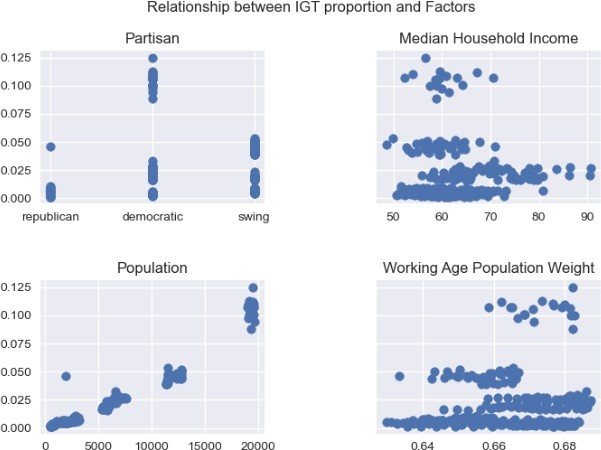
\includegraphics[scale=1]{Chapter-2/Figures/IGT and factors.jpg}
    \caption[IGT and Factors Scatter Plot]{Factor and IGT Scatter Plot
        \texttt{} }
    \label{Figure 2.3}
\end{figure}

\subsubsection{Model Setting}
Though I did a relatively comprehensive literature investigation in grants distribution formula issue, and the sample data includes the most important concerns in intergovernmental transfer distribution, it still possible that some variables may be omitted from the equation, especially given this is a longitudinal data with 19 years time span. So one crutial problem for this investigation is how to deal with the potential omitted variable issue and avoid the following heteroscedasticity and endogenity problem. To make sure I can get an unbiased estimate, I adopt two factor fixed effect model in the regression. In the following researech, I display 3 regression models. The benchmark model is OLS regression. Besides, since the fiscal behavior happens on state level, which is a relatively big and stable jurisdiction, it's totally possible some factors are time-invariant. So, the second model in my display is fixed model with time variable fixed. Though, state is a relatively stable jurisdiction, the time span is relatively long, thus some omitted variables could be time-variant as well. To get all these omitted variables controlled as much as possible, the third model I adopt is two factor fixed effect model, with both time factor and individual effect controlled.

The equation for OLS regression can be displayed as follow.
\begin{equation}
    \begin{split}
        log(igt_{i,t}) & = \alpha + \beta_1 c_{i,t} + \beta_2 p_{i,t} + \beta_3 log(gdp) + \beta_4 log(pl) + \beta_5 log(mhi_{i,t}) \\
        & + \beta_6 wapw_{i,t} + \beta_7 ur_{i,t} +\beta_8 log(prm_{i,t}) + \epsilon_{i,t}
    \end{split}
\end{equation}
$For\ t = 1, 2, 3...T\ and\ i = 1, 2, 3...N $

The second model, which is the fixed effect model with time effect fixed is:
\begin{equation}
    \begin{split}
        log(igt_{i,t}) & = \alpha_i + \beta_1 c_{i,t} + \beta_2 p_{i,t} + \beta_3 log(gdp) + \beta_4 log(pl) + \beta_5 log(mhi_{i,t}) \\
        &+ \beta_6 wapw_{i,t} + \beta_7 ur_{i,t} +\beta_8 log(prm_{i,t}) + \epsilon_{i,t}
    \end{split}
\end{equation}
$For\ t = 1, 2, 3...T\ and\ i = 1, 2, 3...N $

Finally, the third model, which is two factor fixed effect model with time effect and individual effect controlled is:
\begin{equation}
    \begin{split}
        log(igt_{i,t}) & = \alpha_i + \theta_t + \beta_1 c_{i,t} + \beta_2 p_{i,t} + \beta_3 log(gdp) + \beta_4 log(pl) + \beta_5 log(mhi_{i,t}) \\
        &+ \beta_6 wapw_{i,t} + \beta_7 ur_{i,t} +\beta_8 log(prm_{i,t}) + \epsilon_{i,t}
    \end{split}
\end{equation}

$For\ t = 1, 2, 3...T\ and\ i = 1, 2, 3...N $

There are four hypothesis in this investigation, which can be listed as follow.

\textbf{Hypothesis 1–The unified Government Hypothesis}

Unified government means the administrative branch and legislative branch on federal level coming from same party. Unified government is likely to spend a higher overall spending scale since the financial powers are less limited.

\textbf{Hypothesis 2–Party Specific Hypothesis}

Democratic and republican parties have different preferences on the IGT scale. The preference on IGT of different parties is fuzzy here, since two possible inference may be reasonable here. In terms of the scale of government, the democratic party prefers a big government, which would lead to a higher-scale IGT, and the republican party holds the opposite idea. In terms of the administrative structure, democratic government tends to establish a centralized government, whereas republican government prefers a decentralized structure. In this way, we can get a opposite conclusion

\textbf{Hypothesis 3–Alignment Hypothesis}

The allocation of the IGT are affected by the political ideology. The federal government is likely to allocate more IGT to states that are controlled by same party.

\textbf{Hypothesis 4–Battle Ground States Hypothesis}

The competition level between two parties in state would affect the IGT received by that state government. The federal government is motivated to get elected or reelected; thus, the federal government is willing to put resources and supply more public goods to states that matter a lot for their election to get political credits.

The regression results can be summarized as Table \ref*{Table 2.7}
% Table generated by Excel2LaTeX from sheet 'Sheet3'
\begin{table}[H]
    \centering
    \caption{Regression Results Display}
    \begin{tabular}{cccc}
        \toprule
                                        & \multicolumn{1}{p{7.645em}}{Model-1}  & \multicolumn{1}{p{7.5em}}{Model-2}  & \multicolumn{1}{p{8.07em}}{Model-3}  \\
                                        & \multicolumn{1}{p{7.645em}}{Log(igt)} & \multicolumn{1}{p{7.5em}}{Log(igt)} & \multicolumn{1}{p{8.07em}}{Log(igt)} \\
        \midrule
        \multicolumn{1}{p{6.93em}}{c2}  & -0.0161                               & -0.0534                             & -0.0954                              \\
                                        & -0.43                                 & -1.99                               & -1.83                                \\
        \multicolumn{1}{p{6.93em}}{c3}  & -0.0467                               & -0.0352                             & 0.0282                               \\
                                        & -1.4                                  & -1.4                                & -1.09                                \\
        \multicolumn{1}{p{6.93em}}{c4}  & 0.00886                               & -0.0751                             & -0.101                               \\
                                        & -0.19                                 & -2.21                               & -2.67                                \\
        \multicolumn{1}{p{6.93em}}{c5}  & -0.127                                & -0.122                              & 0.-0768                              \\
                                        & -3.31                                 & -3.12                               & -2.87                                \\
        \multicolumn{1}{p{6.93em}}{c6}  & 0.0792                                & 0.0203                              & 0.0351                               \\
                                        & -1.33                                 & -0.47                               & -0.73                                \\
        \multicolumn{1}{p{6.93em}}{c7}  & -0.0125                               & 0.00947                             & 0.0149                               \\
                                        & -0.32                                 & -0.27                               & -0.51                                \\
        \multicolumn{1}{p{6.93em}}{c8}  & 0.0578                                & 0                                   & 0.0767                               \\
                                        & -1.3                                  & 0                                   & -2.15                                \\
        \multicolumn{1}{p{6.93em}}{c9}  & 0.0314                                & 0.0368                              & 0.00131                              \\
                                        & -1.32                                 & -1.21                               & -0.08                                \\
        \multicolumn{1}{p{6.93em}}{c10} & -0.0601                               & -0.0392                             & -0.0318                              \\
                                        & -1.27                                 & -1.2                                & -0.76                                \\
        \multicolumn{1}{p{6.93em}}{c11} & 0.144                                 & 0.127                               & 0.0973                               \\
                                        & -1.6                                  & -1.87                               & -1.5                                 \\
        \multicolumn{1}{p{6.93em}}{c12} & 0.0561                                & 0                                   & 0.0692                               \\
                                        & -1.26                                 & 0                                   & -1.94                                \\
        \multicolumn{1}{p{6.93em}}{c13} & 0.0963                                & 0.078                               & 0.0371                               \\
                                        & -1.96                                 & -1.78                               & -1.07                                \\
        \multicolumn{1}{p{6.93em}}{c14} & 0.0653                                & 0.021                               & -0.00931                             \\
                                        & -0.81                                 & -0.4                                & -0.15                                \\
        \multicolumn{1}{p{6.93em}}{c15} & 0.000495                              & -0.0173                             & 0.00997                              \\
                                        & -0.01                                 & -0.33                               & -0.21                                \\
        \multicolumn{1}{p{6.93em}}{c16} & 0.0466                                & 0                                   & 0.0512                               \\
                                        & 1.94                                  & 0                                   & 2.44                                 \\
        \bottomrule
    \end{tabular}%
    \label{Table 2.7}%
\end{table}%

% Table generated by Excel2LaTeX from sheet 'Sheet3'
\begin{table}[htbp]
    \centering
    \caption{Regression Results Display (follow up)}
    \begin{tabular}{p{6.93em}ccc}
        \toprule
        \multicolumn{1}{c}{}          & \multicolumn{1}{p{7.645em}}{Model-1}  & \multicolumn{1}{p{7.5em}}{Model-2}  & \multicolumn{1}{p{8.07em}}{Model-3}  \\
        \multicolumn{1}{c}{}          & \multicolumn{1}{p{7.645em}}{Log(igt)} & \multicolumn{1}{p{7.5em}}{Log(igt)} & \multicolumn{1}{p{8.07em}}{Log(igt)} \\
        \midrule
        Democratic States             & 0.259                                 & 0.217                               & 0                                    \\
        \multicolumn{1}{c}{}          & -4.88                                 & -5.51                               & 0                                    \\
        Swing States                  & 0.0899                                & 0.0189                              & 0                                    \\
        \multicolumn{1}{c}{}          & -2.7                                  & -1.94                               & 0                                    \\
        Log(population)               & 0.106                                 & 1.087                               & 0.457                                \\
        \multicolumn{1}{c}{}          & -0.92                                 & -10.67                              & -1                                   \\
        working age population weight & -5.362                                & 2.199                               & -4.768                               \\
        \multicolumn{1}{c}{}          & -6.93                                 & -2.72                               & -5.43                                \\
        Log(median household income)  & -0.753                                & -1.407                              & -0.348                               \\
        \multicolumn{1}{c}{}          & -3.51                                 & -8.68                               & -1.26                                \\
        unemployment rate             & 0.0136                                & -0.0151                             & 0.0234                               \\
        \multicolumn{1}{c}{}          & -1.97                                 & -2.27                               & -4.51                                \\
        Log(GDP)                      & 0.807                                 & -0.0855                             & 1.346                                \\
        \multicolumn{1}{c}{}          & -6.85                                 & -0.86                               & -7.43                                \\
        Log(mileage)                  & 0.143                                 & 0.0576                              & 1.222                                \\
        \multicolumn{1}{c}{}          & -2.91                                 & -1.59                               & -3.21                                \\
        Constant                      & 9.057                                 & 7.078                               & -1.473                               \\
        \multicolumn{1}{c}{}          & -15.21                                & -14.32                              & -0.73                                \\
        \midrule
        Observations                  & 309                                   & 309                                 & 309                                  \\
        Adjusted R2                   & 0.942                                 & 0.969                               & 0.68                                 \\
        \bottomrule
    \end{tabular}%
    \label{Table 2.8}%
\end{table}%

\subsubsection{Result Analysis}
The first information in the display is that all there models show high adjusted $R^2$, especially the first two models. The high adjusted $R^2$ could be explained by the high explanatory power in the control variables I selected. The adjusted $R^2$ of the third model, in which both time and individual effect controlled, is relatively lower. Given that the state variable is controlled and one of the criterion of the sample selection is that the partisan of the states has not changed in the past 19 years, the deduction process in the fixed effected regression would delete the partisan variable that's the reason why coefficients of partisan variables are 0. Thus the lower adjusted $R^2$ can be explained by the loss of partisan variables. So for the rest of analysis, I'll adopt the coefficients of partisan variables in model 2 and all other coefficients in model 3.

From model 3, $ c_4(r, r, d, d), c_5(r, d, r, r), c_{16}(d, d, d, d)$ are statistically significant on 5\% significant level. From model 2, the partisan variables, "Democratic States" and "Swing States", are significant as well. If we loosen the 5\% significant level to 10\%, $c_2(r, r, r, r), c_{12}(d, r, d, d)$ is also significant.

The first hypothesis about the unified government is supported by the regression result. By comparing the coefficient of $c_5(r, d, r, r)$ and $c_1(r, r, r, r)$, we can tell that a traditional republican state, with both administrative and legislative branch controlled by republican party, receives 7.78\% lower of intergovernmental transfer under bipartisan control on federal level compared to a unified republican controlled federal. When the federal level is not uniformly controlled by the republican party, the ability to distribute grants to state level is significantly constrained.

The second hypothesis about party preference is also supported by the significant coefficients. Comparing the coefficient of $c_{16}(d, d, d, d)$ and $c_1(r, r, r, r)$, I can tell that states receive 5.12\% higher intergovernmental transfer when both federal and state level are controlled by democratic party compared to when both federal and state are controlled by republican party.This means that democratic party prefer to transfer more to state government, the first inference in my hypothesis dominates. The understanding of this result needs more investigation though. For example, does this conclusion still holds when it comes to the intergovernmental transfer to local level?

Alignment effect is also significant in intergovernmental transfer distribution, compared aligned combination $c_1(r, r, r, r)$ and $c_16(d, d, d, d)$, coefficients for all other unaligned combinations, including $c_4(r, r, d, d), c_5(r, d, r, r), c_{16}(d, d, d, d)$ are negative.

Finally, about the effect of partisan, the coefficient of swing states in model 2 doesn't support my hypothesis about battle ground state. One possible explanation is that we do not have a factor to control the effect of election period. My theoretical analysis and the supporting literature about the benefits swing states have is achieved by the election process, however this investigation is a longitudinal study with 19-years time span, thus for those years when politicians do not care about elective pressure and political credit, the benefits of swing states may be neglected.

\subsubsection{Deficiencies and Rethinking on Related Topics}
I have to admit that our investigation is limited and deficient. The most obvious defect is the time span of the data. This defect may be even more serious given that elections happens every 2 even 4 years, not annually. One may claim that our model is not convincing since our conclusion may not hold when put our investigation in a longer time span.

Given all the deficiencies we talked about, this paper could be an extension and may get some insight in related area. The investigation on IGT is embed in the framework of fiscal federalism. Given all the benefits of fiscal federalism as Musgrave \cite{musgrave1971economics} mentioned, it also introduces several challenges. Our investigation may supply some implication for those challenges. For one, The involvement of multiple jurisdictions in the funding and execution of public programs introduces loss aversion behavior between the national and the subnational governments \cite{alesina2019loss,bourdeaux2018loss,rees2014loss} and asymmetric information \cite{brennan1987efficient,huber2006optimal,miller1985dividend}. The former problem arises because the subnational are less accountable for the local government separation of funding and spending responsibilities. Information and potential loss aversion creates the risk that agency problems compromises the allocative efficiency of federal spending, including conflict of interest and moral hazard problems. For example, the presence of moral hazard problems act to discourage the subnational government from delivering services cost effectively \cite{williams2021moral}(i.e., a shirking).

Moreover, the delegation of program implementation from a central government to a subnational government, increases information asymmetry, which may further exacerbate the above incentive problem. They may also increase the risk that agents within a subnational government engage in behaviors that are inconsistent with program goals (i.e., conflicts of interest problems). Our analysis suggests some potential explanation. Our investigation confirmed the effect of political party bias in grants distribution. This effect may be a common knowledge for both federal and state governments. Once the state government know the grants they received is guaranteed, the state government won’t be motivated enough to implement the policy dedicatedly. So the incentive problem may be partly explained by the biased grants distribution process.

Finally, this research may be a supplementary material for the flypaper effect, which I will discuss in detail in the following chapter.The fly paper effect means that increase in grants-in-aid leads to significantly higher public spending than the same increase of private income, so money sticks where it hits \cite{inman2008flypaper}. Scholars ascribe this fact to many causes.Hamilton tried to explain fly paper effect as improper data distinguishment or improper empirical method \cite{hamilton1986flypaper}.Some identify flypaper effect happen due to fiscal illusion \cite{gramlich1997stimulative}. Our research may offer some mew angle to understand the flypaper effect. The confirmed biased effect in grants distribution means for some of the states, getting grants from federal governments is effortless compared to getting revenue from other methods. This relative price effect may explain the fact that state government prefer to raise funds from IGT rather than raising tax.

\section{Summary}

    \chapter{Political Party Control and Intergovernmental Grants: a Panel Data Analysis}


\section{Introduction}
The strategic dynamics that exist between different tiers of governments have long been a focal point of fiscal federalism, particularly as they relate to the allocation of intergovernmental transfers \parencite{agrawal2022local,dahlby1996fiscal,gordon1983optimal}. In the fiscal federalism literature, these dynamics refers to how governments at different levels (e.g., federal, state, and local) elect to respond when their choices are influenced by another government's choices.  For example, a federal government that elects to transfer funds through a program that requires a certain level of matching from a subnational government (rather than through a general transfer program) may elicit the subnational government to accept or reject the grant offer. Given the presence of such dynamics, it is critical that they be considered in the design of intergovernmental transfer (IGT) programs \parencite{dahlby1996fiscal,gordon1983optimal}. A failure to properly consider how they affect fiscal behaviors can induce distortions that reduces the effectiveness of government spending, such as overspending by subnational governments or temporary adjustments in tax collections\parencite{bailey1998flypaper,inman2008flypaper,turnbull1998overspending}.

Academic interest in IGTs has produced a series of studies that offer insights into the complex negotiations and compromises that often characterize the IGT distribution process\parencite{chubb1985political,dixit1995redistributive,weingast1979rational}. Many of the investigations are based on game theory, which assumes that bargaining is carried out by rational players\parencite{banks2006general,baron1989bargaining,martin2018dividing}. However, a limitation of the game-theoretic approach is that it is often grounded in a rational choice paradigm that is at odds with the realities of the environment within which IGTs are distributed. To account for the complex reality of IGT, it is often necessary consider an array of additional factors that goes beyond assumptions of rationality and homogeneity\parencite{golden2008pork,milligan2005regional,petry1999electoral,tellier2006public}. \textcite{rosenstiel2021congressional}, for example,points to the need to consider factors such as partisan alignment and preferences for grant categories.

The purpose of this research is to add to the extant body of literature IGTs by examining how political party control affects federal government IGT distributions. Political party control remains a largely unexamined independent variable in analysis of IGT distributions in the US context. In the literature review that was conducted as part of this study, only two previous studies were found that explicitly addresses this topic\parencite{ansolabehere2002equal,ansolabehere2006party}. This research contributes to this stream by examining the influence of four distinct features of political party control are considered including (1) whether the federal government is unified, (2) the specific party in control, (3) political alignment across the federal and state governments, and (4) political competition across parties.


The analysis is conducted, using a fixed-effect regression model. Using panel data collected from 14 states, we find that political alignment significantly impacts the distribution of intergovernmental grants. Specifically, states with a unified government, where both the administrative and legislative branches at the state and federal levels are controlled by the same party, tend to experience variations in grant allocation. Republican-controlled states under a unified Republican federal government receive a reduced proportion of grants compared to states under bipartisan or Democratic control. Furthermore, our analysis indicates that swing states receive significantly less grant funding compared to their partisan counterparts in non-election years. This suggests a strategic behavior of federal governments, which may allocate resources not solely based on states' needs or economic conditions but also influenced by political considerations and party alignment.

These findings are important because of the scant research that surround the role of political party control in IGT distributions. Despite the presence of a relatively healthy body of theories stream of research that examine the influence of various stakeholders on budget outcomes, this independent variable remains largely unexamined in the US federal context\parencite{patashnik2000budgeting}.  It is also significant due to the significant role that politics play in the budget process. The budget is by many viewed as the prime expression of political preferences. \textcite{wildavsky2003new} viewed budgeting as the basic framework that makes decision-making in political environments possible.  He articulated the role of politics in budgeting as follows: “All Budgeting is about politics, most politics is about budgeting, and budgeting must therefore be understood as part of a political game.”

% Fiscal federalism has long been a focal point within the realm of public finance, particularly concerning the strategic dynamics between various tiers of government\parencite{gordon1983optimal,dahlby1996fiscal,agrawal2022local}.
% The allocation of intergovernmental transfers within this domain emerges as a critical area of inquiry, given its potential to profoundly influence governmental fiscal behavior and potentially lead to distortions\parencite{dahlby1996fiscal,gordon1983optimal}. For instance, these grants may induce overspending by subnational governments or stimulate/retard state governments' tax collection behavior\parencite{inman2008flypaper,bailey1998flypaper,turnbull1998overspending}. This paper seeks to unravel a fundamental question within the realm of American fiscal intergovernmental transfer: does the distribution of federal grants reflect the influence of party preferences and alignment between federal and state governments, as well as party attributes at the state level? These concerns pivot around the potential for federal bias favoring states with matching political affiliations, a significant inquiry given grants' role as 20\% of federal annual revenue \parencite{rosenstiel2021congressional}.


% Empirical investigation into the grants allocation of funds has delineated the complex negotiations and compromises that characterize grant distribution---a process described not merely as top-down decisions, but as federative conciliation \parencite{chubb1985political, 1976A, dixit1995redistributive}. Our focus narrows upon federal decision-making, assuming the compliance of subnational governments---a perspective less explored but critical in the intricate hierarchy of government interactions. The traditional investigation on the bargaining on federal level, often based on game theory, propose rational, identical players \parencite{baron1989bargaining, banks2006general, martin2018dividing}, but the diversity of stakeholders involved introduces an array of additional considerations\parencite{milligan2005regional, golden2008pork,tellier2006public, petry1999electoral}.
% Factors such as partisan alignment and preferences for grant categories are part of this multifaceted equation\parencite{rosenstiel2021congressional}, each contributing to the complex reality of grant distribution.

% This paper seeks to address gaps in the literature by empirically investigating the effects of party preference and alignment between federal and state governments, as well as state party affiliation, on intergovernmental transfer distribution. In addition, we want to distinguish whether the alignment effect, if it's significant, is due to the federal level's subjective favoritism towards states with similar party affiliations. By dissecting panel data spanning various states and political contexts, this paper will highlight how such political dynamics manifest in the actual allocation of federal funds.

% In Chapter 3, the dissertation takes a critical turn to explore the nuanced effects of political party control on the distribution and utilization of intergovernmental grants within the United States, a pivotal component of the fiscal federalism framework. This analysis directly supports the overarching aim of the dissertation to unravel the complex dynamics of fiscal interactions between central and subnational governments, by focusing on the political dimensions that underpin these interactions. By employing a panel data analysis over a 19-year period, this chapter sheds light on how political alignment and party control significantly influence the flow of intergovernmental transfers, adding a critical layer of understanding to the strategic fiscal behaviors of governments within the federal system. This exploration not only enhances our comprehension of fiscal federalism's theoretical and practical applications but also underscores the importance of political considerations in the design and execution of fiscal policies. As such, the findings from this chapter contribute to a more nuanced understanding of fiscal federalism and intergovernmental transfer, enriching the dissertation's holistic examination of governmental fiscal strategies and their implications for public service delivery across different tiers of government.

% Following this introduction, a comprehensive overview of the grant distribution rules in the United States will set the platform for our narrative. We will then proceed with a robust literature review to carve out the missing pieces in the existing body of research. Our research questions and hypotheses will be postulated with precision and academic rigor, subsequently leading to a dialogue on our research methodology and an analysis of the findings in pursuit of academic and practical enlightenment.


\section{Intergovernmental Grants: A Background}
Consistent with recent trends in the academic literature\parencite{abbott2012intergovernmental,akai2019role,lago2024effects}, this paper uses the terms intergovernmental transfers and grants interchangeably to depict fiscal handovers from one government tier to another. In federal systems, such handovers serve as a multifunctional fiscal instrument, designed to not only instill spending in national-priority sectors but also to harmonize fiscal imbalances across regions. Intergovernmental transfers are therefore often viewed as being instrumental in strengthening subnational entities, and in addressing regional inequities, including vertical disparities rooted in structural differences and horizontal inequities emanating from diverse fiscal capacities and expenditure requirements of sub national jurisdictions.

The process through which intergovernmental transfers are distributed is often depicted through the lenses of a game-theoretic bargaining game. Such a framework is helpful because it captures the strategic dynamics that surround the distribution of intergovernmental grants in democratic environments, and that continues to be a focal point of fiscal federalism\parencite{agrawal2022local,dahlby1996fiscal,gordon1983optimal}. These dynamics refers to how governments at different levels (e.g., federal, state, and local) elect to respond when their choices are influenced by another government's choices.  For example, a federal government that elects to transfer funds through a categorical transfer program that requires a certain level of matching from a subnational government (rather than through a general transfer program) may influence whether subnational government elects to accept or reject the grant offer. Extant research show that consideration of strategic dynamics is a critical determinant of the success of intergovernmental grants (IG)\parencite{dahlby1996fiscal,gordon1983optimal}. If not accounted for, they may cause fiscal behaviors that reduces the effectiveness of government spending, such as overspending by subnational governments or temporary adjustments in tax collections\parencite{bailey1998flypaper,inman2008flypaper,turnbull1998overspending}.

Over time, important advances have been made to further refine these frameworks in ways that that make them more capable of capturing the strategic dynamics that surround intergovernmental transfers. A seminal contribution in this regard is a paper by \textcite{baron1989bargaining}, which laid the foundation for much of the subsequent work. It depicts the distribution of grants as a bargaining game among different decision-making groups, when one participant in the game is the decision-making institution, such a congress or a specific committee. \textcite{baron1989bargaining} bargaining framework is built around four rules that are regarded as crucial to simulations of the bargaining process that determines grants distribution. These include the recognition rule, voting rule, amendment rule, and money-distribution rule.


\begin{enumerate}
    \item The recognition rule determines how to select the agenda setter that make the initial proposal. In the extant literature, most simulations are grounded on the random recognition rule, which assumes that members of the decision-making institution have equal probabilities of being chosen to make the initial proposal\parencite{anesi2015bargaining, diermeier2011legislative,kalandrakis2004three,rosenstiel2021congressional}.
    \item The voting rule establishes the standard for passing the proposal, with the majority rule and unanimous voting rule being common assumptions\parencite{baron1989bargaining}.
    \item The amendment rule places constraints on making amendments, ranging from the closed rule (allowing no amendments) to the open rule (allowing any and all germane amendments).
    \item The grants-type rule determines how grants could be manipulated by decision-making institutions, with some scholars assuming direct decisions on the number of receivers, referred to as "earmarks" spending models.
\end{enumerate}

\textcite{baron1989bargaining}'s foundational paper also established several important assumptions that accompanied their framework, such as random recognition, majority voting rule, and earmarks rule. Their work, along with a subsequent study by \textcite{banks2006general}, offers three key insights. First, it demonstrates that legislators with agenda-setting power tend to receive a disproportionate share of funding. Second, it demonstrates that, when in a state of equilibrium, funds flow only to legislators in the winning coalition, with no funds allocated to those outside of it. Third, they found that when proposals are brought up under a closed rule, the winning coalition is minimized, leading to the maximization of benefits for the members of the winning coalition.

More recently, a study by \textcite{martin2018dividing} added to \textcite{baron1989bargaining}'s framework by modifying the assumptions of the model, including its heavy reliance on “earmarks.” Martin's modified model placed limits on decision-makers' power to determine the factors in the formula rather than the specific numbers. This modification generates a model that is more closely aligned with the realities of political and administrative life. It also produces two conclusions that differs from those of Baron and Ferejohn's model. First, in contrast to the original model, Martin's model predicts oversized winning coalitions and the emergence of persistent winning blocs. Additionally, \textcite{martin2018dividing} demonstrates that when bargaining occurs over a low-dimensional formula  ,  (i.e, less than five variables included in the formula) legislators have limited ability to target funds to specific districts; a prediction supported by empirical evidence. For instance, Martin analyzed existing formula grants and found that 95\% of the formulas have fewer than 5 variables, indicating limited bargaining dimensions for members. Consequently, some jurisdictions can be free riders, even if they are not part of the winning coalition. Based on these findings, Martin predicts a positive distribution outside the winning coalition.

However, there are several limitations with applying game-theoretic models to explain IGT distributions. Many of these arise from the fact that they often are grounded in a rational choice paradigm that is at odds with the realities of the environment within which IGTs are distributed. To account for the complex reality of IGT, it is often necessary consider an array of additional factors that goes beyond assumptions of rationality and homogeneity \parencite{golden2008pork,milligan2005regional,petry1999electoral,tellier2006public}. \textcite{rosenstiel2021congressional}, for example, points to the need to consider factors such as partisan alignment and preferences for grant categories.

\section{Political Party Control and IGT Distributions: Literature Review }

As noted in the introduction, the purpose of this paper is to examine how the distribution of political party control affects IGT distributions in the US federal budgetary context.  In the literature review that was conducted as part of this study, two previous studies were found that explicitly addresses this topic\parencite{ansolabehere2002equal,ansolabehere2006party}. Both studies are confined to examining aspects of party control on intergovernmental distributions from state governments to counties. The earlier study \parencite{ansolabehere2002equal} examined the distribution of funds from money by states to counties. Using cross-sectional analysis, it showed that the proportion of legislative seats per person was positively related to the amount of transfers a county received from the state per person. The more recent study \parencite{ansolabehere2006party} examined the distributive expenditures across counties in US states over a 40-year period. The study shows that (1) counties that traditionally support (in terms of vote share) the governing party tend to receive larger shares of state transfers, and (2) that the distribution of IGTs tends to follow the direction of the shifts across governing parties.

\textcite{borck2003political} investigates the impact of political factors on the distribution of intergovernmental grants through modeling and empirical data analysis. The core of the research focuses on local government officials lobbying the central government to secure more funding. The article proposes that lobbying costs increase with the geographic and political distance from the central government, theoretically leading to a decrease in grant allocation with increased distance. Their Empirical analysis using county-level data from California finds a negative correlation between grant allocation and geographic distance, aligning with the hypothesized political access costs. Furthermore, the study observes that regions politically aligned with the central government tend to receive more funding. During the response of Covid-19 pandemic in America, \textcite{terman2015performance,terman2020getting,terman2015improving,terman2022even}'s series of studies extensively examines how political alignment, partisan relations, and administrative capabilities impact the distribution and efficiency of federal funds. Her findings highlight the significant role of partisan congruence in enhancing the effectiveness of policy implementation during crises like the COVID-19 pandemic.

Similar analysis is also found outside America, \textcite{sole2008effects}explore the influence of partisan alignment with upper-level governments on local funding in Spain, demonstrating that local units aligned with higher government tiers tend to receive more funding.   These research highlights the significance of political motives in the distribution of intergovernmental grants, showing that the actual allocation of government funding can deviate from ideal efficiency levels due to political influences, even in areas with evident public service spillover benefits.

Besides, a series of studies were produced in the 1970s and 1980s that examined whether party control was related to increases in spending on programs that were ideologically preferred by a particular party. \textcite{carlino2023partisanship} find that Republican governors are less inclined than their Democratic counterparts to spend on federal intergovernmental transfers. As a result, states led by Republicans tend to have lower debt levels, delayed taxation, and initially lower economic activity. Overall,  At the state level,
these studies offer limited evidence in support of such influence \parencite{fry1970politics,winters1976party,plotnick1985politico,  lowery1987distribution, marquette1981competition, plotnick1990party}. However, at the federal level a stronger correlation was found \parencite{owens1984federal,browning1973geography,levitt1995political, ritt1976committee,kiewiet2002here, ansolabehere2006party}. In addition to this latter finding, this stream of research is valuable in that it offers insights into how
to operationalize studies of political control (see methods section).

Explicitly stated, this research adds to the above literature by examining the role of political party control in IGT distributions from the US federal government to the states. In the U.S. federal context, intergovernmental grants are typically classified along two dimensions \parencite{clemens2023intergovernmental,dilger2015federal}, including (1) the level of control that federal agencies exercise in terms of directing how grant funds are used by a subnational government, and (2) the methodologies employed to determine grant amounts or grant shares. The former dimension can be used to categorize three common grant types including categorical grants, block grants and general revenue sharing grants. Among these grant types, categorical grants provide federal agencies with the highest level of control and influence over how state and local government spend awarded funds. They often come attached with language that narrowly defines the purposes for which a subnational government may spend distributed funds.

Block grants signify the distribution of funds that are earmarked for a specific program or project, rather than a narrowly defined spending purpose. Federal agencies exercise less control over block grant programs, compared to categorical grant programs, given that they are earmarked at the program level. For the recipient, they constitute a relatively flexible pool of funds permitting the recipient subnational government to tailor the design and implementation of programs in response to identified regional needs \parencite{finegold2004block}.

Finally, general revenue sharing grants refer to grants that are apportioned to subnational governments, using a part of a central government's tax revenues. Sometimes referred to as unconditional grants, they impose very few restrictions on recipient subnational governments. They are distributed to subnational governments through some form of pre-defined formula, defined by law, where the receiving units may or may not be required to match the amounts received\parencite{larkey2015evaluating}. Given that general revenue sharing grants are based on a predefined formula, they extend very limited opportunities for federal agencies to control or influence the distribution of federal funds.


The second dimension mentioned above is the methodologies employed to determine grant amounts or grant shares. Based on this dimension, relevant grant types include project grants, formula grants and reimbursement grants. Project grants refer to grant funds distributed to fund particular projects or deliverables. This grant type is awarded through a competitive process, encouraging states to
propose and execute exemplary projects\parencite{dilger2015federal}.Formula grants are noncompetitive grants that are allocated to subnational governments based on a pre-defined formula. Such formulas often consider a variety of economic and social characteristics within a jurisdiction\parencite{huffman2006formula}. Whether formula grants eliminates political motives in resource distribution is unclear yet. \textcite{banful2011formula} delves into whether Ghana's implementation of the formula-based District Assemblies Common Fund (DACF) effectively eliminates political motivations in intergovernmental grants. The findings indicate that despite the formula-based allocation mechanism, political factors still play a significant role in the distribution of the District Assemblies Common Fund. Especially around elections, the government tends to allocate more funds to key or politically sensitive areas. This suggests that despite the system's design for fairness, political motivations can still influence the actual distribution of resources.   Finally, reimbursement grants reimburse state and local governments for a portion of their expenditures on specific programs. They are awarded using open-ended and closed-ended matching grant variations.


In this paper we propose that political party control is channeled into IGT distributions through the level of control that central government agency officials and legislators exercise over such distributions. At the administrative level, this level of control is defined through the laws that accompanies different types of grant programs. For example, non-discretionary grant programs, where allocations are determined by a set formula, offers limited opportunities for federal agencies to control and influence distributions. On the other end, categorical grant programs often extend substantial control to the administrative agencies.

The previously mentioned dimensions used to classify intergovernmental grants provide a useful framework for depicting the level of discretion that accompanies different grant types. Figure \ref{grantstype} depicts the different grant type possibilities, using a two-dimensional matrix. It suggests that the control that federal agencies and administrators exercise over grant distributions reaches its zenith with categorical project grants. This grant form extends substantial authority to the federal agency in terms selecting recipients and determining grant amounts. Reimbursement grants, while less directly controlled, provides some opportunities for federal agencies to steering benefits towards preferred states.

According to the Congressional Research Service, federal agencies distribute federal funds via close to 600 federal grant programs\parencite{dilger2015federal}. Close to 70 percent of these programs is some form of project grant\parencite{dilger2015federal}. Hence, a substantial portion of intergovernmental grants are distributed through grant programs where federal agencies exercises substantial levels of control over grant distributions.

At the legislative level, the influence over grant distributions occurs at the time when legislators establish the basic parameters that guides grant distribution for the various programs. For example, the selection criteria embedded in formula grants can be oriented to favor certain constituencies that reflects legislators' preferences\footnote{While the selection criteria embedded in formula grants can be oriented to favor certain constituencies, such criteria would reflect legislators' preferences at a time that precede the distribution, rather than preferences during the distribution year, presuming these do not coincide.}. It may also occur indirectly through pressure that legislators impose on administrative agencies.

\section{Hypothesis}

To examine the general proposition that political party control influence IGT distributions, this study considers four factors that we argue captures important aspects of party control. These include (1) whether the federal government is unified, (2) the specific party in control, (3) political alignment across the federal and state governments, and (4) political competition across parties. These factors were included because they have been identified as features of political party control in previous research.

The first feature of political party control that is considered is whether the federal government is unified or not. A unified government is characterized by the alignment of the administrative branch and legislative branch at the federal level under the same political party. A unified government is a feature of political party control, given that  it reduces the need for political compromises across parties. \textcite{coleman1999unified} states that a unified government is productive in public policy outcome. Given this, such alignment is argued to result in higher overall spending. Explicitly stated, the first hypothesis is:

\textbf{Hypothesis 1: A unified federal government is positively associated with higher overall IGT spending.}

The second feature of political party control that is considered is the specific party in control. The Democratic and Republican parties are presumed to exhibit distinct preferences regarding the scale of IGTs\parencite{weaver2010paths,winters1976party}. However, it is challenging
to interpret these differences in party preferences toward IGTs. The Democratic Party tends to favor a larger and more centralized government and the republican party tends to favor a smaller and more decentralized government. The Democratic party's preference toward a larger government suggests a positive association with IGT spending. At the same time, the Republican party's preference for decentralization goes hand in hand with IGTs.Consequently, these contrasting preferences lead to divergent conclusions. Given this, the second hypothesis is:

\textbf{Hypothesis 2: Political party color is related to the level of IGT spending.}

The third feature of political party control is the level of political alignment across the federal and state governments. Research by \textcite{ansolabehere2006party} show that hat counties that traditionally have supported the governing party (in terms of vote share) receive a larger share of
state transfers to local government. They also find evidence that counties with greater legislative seats per person receive more transfer payments from state governments\parencite{ansolabehere2002equal}.In this research, we test whether a similar effect is present in the context of IGT transfers from the federal government to state governments. Explicitly stated, we hypothesize that:


\textbf{Hypothesis 3: The level of political party alignment across the federal and state governments is positively related to IGT distributions.}

The final feature of political party control that is considered is whether a state is a battle ground state or not. The federal government, driven by the motivation to secure election or reelection, is inclined to allocate resources and provide additional public goods to states that significantly influence electoral outcomes. This strategic allocation is aimed at accruing political credits. \textcite{veiga2013intergovernmental} reveal how intergovernmental fiscal transfers are utilized as political tools during electoral cycles, with increased transfers to certain regions to boost political support in election years. \textcite{dahlberg2002vote} analyze the strategic allocation of intergovernmental grants in Sweden before elections, supporting the Lindbeck-Weibull/Dixit-Londregan model that governments allocate more funds to areas with a high number of swing voters.Therefore, we argue that swing states are more likely to secure IGTs. Explicitly stated, the final hypothesis is:

\textbf{Hypothesis 4: Battle ground states are more likely to secure IGTs compared to non-battle ground states.}

%%%%%%%%%%%%%%%%%%%%%%%%%%%%%%%%%%%%%%%%%%%%

\section{Research Approach}


To test the above hypotheses, we undertook a two-step analytical approach. The first step was conducted using a principal components analysis (PCA). This step was conducted for purposes of establishing the extent to which IGT distributions are driven by shared economic and social
attributes among same-party states. This step was added to the analysis as a result of \textcite{martin2018dividing} observation that biases in IGT distributions may partially be driven by shared economic and
social attributes among same-party states, given that such attributes often determine grant distributions established by formulas. The second step centered on testing the above four hypotheses. Toward this end, we conducted a fixed regression analysis based on the panel data of states in America.


% In the context of this study, the disparities in the distribution of intergovernmental transfers and their link to political party attributes may stem from two distinct reasons. Firstly, the alliance effect, which is subjective in nature, suggests that higher-level governments prefer to allocate more funds to lower-level governments that share the same political party affiliation. The second reason revolves around a preference for certain economic and social development policies by higher-level governments, thereby benefiting all lower-level governments that exhibit specific economic and social characteristics. Often, these shared economic and social attributes align with political party affiliations. To achieve the research objective, namely, to ascertain the presence of the first reason, it is imperative to examine the validity of the second reason before employing regression analysis to investigate the relationship between disparities in transfer payments and political party attributes. If the influence of the second reason holds, meticulous control is necessary to disentangle its effects from those attributed to alliance effects. Thus, the application of Principal Component Analysis (PCA) prior to regression analysis serves a crucial role. It allows for the investigation into whether variations in transfer payments are merely a reflection of economic and social characteristic preferences, which coincidentally align with political affiliations. This step is fundamental in ensuring that our analysis accurately identifies the influence of subjective political alliances, free from the confounding impact of shared economic and social traits across different political administrations.


\subsection{Step 1: Principle Components (PCA) Analysis}

In the context of this study, disparities in the distribution of IGTs may stem from two distinct effects. The first effect, which we refer to as the alliance effect, is assumed to arise from a higherlevel government's preference toward allocating funds to lower-level governments that share its political party affiliation. The political party control features that are examined in this research are assumed to generate alliance effects. The second effect, which we refer to as the preference effect arises from a higher-level government's preferences toward funding certain economic and social development policies. In terms of IGT distributions, this effect benefits lower-level governments
that exhibit certain economic and social characteristics. These shared economic and social attributes may align with political party affiliations. More specifically, numerous American and international studies have provided evidence indicating that factors such as economic structure and economic
conditions influence political affiliation. Therefore, it is plausible to infer that the reverse logic holds true: regions governed by the same political party may also share similar economic and social structures\parencite{Alan2009Partisanship,anderson2006economic,weatherford1978economic}. Given this, it becomes important to examine the potential influence of the preference effect, before employing regression analysis to investigate the relationship between disparities in transfer payments and political party attributes. If
it is established that the preference effect is prevalent, additional controls are necessary to disentangle its effects from those attributed to alliance effects. Hence, the application of PCA prior to regression analysis serves this crucial role. That is, it allows us to determine whether variations in
transfer payments are merely a reflection of economic and social characteristics that coincidentally align with political affiliations.

A PCA is a statistical technique that allows researchers to simplify the complexity of highdimensional data while retaining trends and patterns. It allows for this by transforming the original variables into a new set of uncorrelated variables, referred to as the principal components. These
principal components are ordered so that the first few variables retain most of the variation present in the original variables. PCA is particularly useful when analyzing data with numerous interrelated variables to identify underlying structures within the data. For purposes of this research, it allows us
to reduce the dimensionality of data, and improves interpretability while minimizing information loss. By focusing on the principal components with the highest variances, it allows us to discern the most significant patterns and relationships within the data.

It is useful to apply when analyzing data with numerous interrelated variables to identify underlying structures within the data. This method is particularly beneficial in reducing the dimensionality of data, improving interpretability while minimizing information loss. By focusing on the principal components with the highest variances, researchers can discern the most significant patterns and relationships within the data.

The primary aim of the PCA that was conducted as part of this study was to distill economic and social characteristics of states into a manageable number of components that could reveal potential clustering by political affiliation. To accomplish this, we (1) standardized the dataset to ensure each
variable contributed equally to the analysis; (2) computed a covariance matrix to identify relationships between variables; and (3) extracted eigenvalues and eigenvectors to determine the principal components. Following these three steps, the resulting components were analyzed to determine the extent to which they captured the variance in our data, thereby guiding us in determining the number of dimensions needed for further analysis. This latter step was crucial for isolating the shared economic and social attributes among same-party states. It provided a foundation for understanding how these attributes might influence IGT distributions beyond the surface level of political alignments and preferences.


\subsubsection{Data and variables for PCA Analysis}
The primary variables required mainly consist of economic and social characteristics at the state level, with particular emphasis on variables frequently appearing in transfer payment formulas. Additionally, as this article specifically focuses on the economic and social commonalities among states governed by the same political party, a grouped sampling method was adopted for selecting sample states. All states were categorized into traditional Democratic states, traditional Republican states, and traditional swing states. Within each group, 5-6 states were randomly selected as samples. The economic and social variables of all selected sample states were then analyzed for annual changes from 2000 to 2019, thus forming a panel dataset.

The state grouping method relies on two primary criteria: historical presidential election outcomes and their corresponding winning percentages, a methodology delineated in \textcite{beachler2015presidential}. Democratic and Republican states are characterized as those consistently favoring a particular party in presidential elections since 1984, where the winning rates surpass 58\%. Swing states are recognized as those that have alternated between parties in selecting presidents, with winning rates falling below 58\%. The states encompassed within the analysis are enumerated in Table \ref{Table 2.3}.


The social and economic characteristics commonly included in the formula for intergovernmental transfers encompass population, working-age population weight, median household income, unemployment rate, road mileage, and GDP per capita \parencite{dilger2015federal}. I gathered all factors mentioned in \Textcite{dilger2015federal}'s study for the sampled states. Additionally, I referenced major intergovernmental transfer programs such as Medicaid, the Title I-A education program, Temporary Assistance for Needy Families (TANF), Section 8 Housing Choice Vouchers, and the Community Development Block Grant (CDBG) to comprehensively collect factors. To ensure data convenience for regression and enhance data visualization, I performed appropriate operations. The collected characteristics and data sources are detailed in Table \ref{Table 2.4}.%%%%%%chatgpt checked%%%%%


\subsubsection{PCA Process and Results}

Issues of correlation across the collected variables are evident. For example, the weight of the working-age population and the unemployment rate are highly interdependent. Moreover, higher population levels inherently correspond to increased usage of public roads. This observation is further corroborated by the correlation heatmap, depicted in Figure \ref{heatmap},which indicates a certain degree of correlation among the variables. As such, we conclude that PCA is needed to reduce data dimensionality and mitigate issues of multicollinearity.%%%%%chatgpt checked%%%%%

% \begin{figure}
%     \centering
%     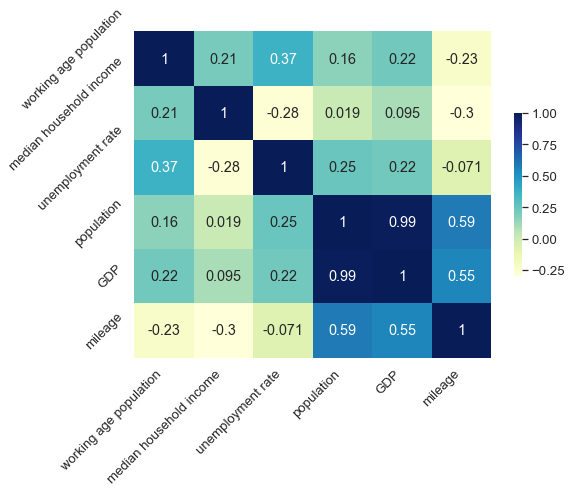
\includegraphics[scale=0.7]{Chapter-3/Figures/heatmap.png}
%     \caption[Heatmap of the Social Characteristics]{Heatmap of the Social Characteristics
%         \texttt{} }
%     \label{heatmap}
% \end{figure}

To address the first question, the apparent hindrance lies in the difficulty of directly assessing the similarity of jurisdictions in social and economic characteristics. To overcome this challenge, I employed Principal Components Analysis (PCA) to reduce data dimensionality and mitigate issues of multicollinearity. This approach aims to determine whether the reduced-dimension data exhibit cluster distribution or scattered distribution.

The results of the PCA variance analysis, as depicted in the figure, reveal that the first two dimensions encapsulate 67\% of the information, while the first three dimensions account for 87\% of the information.
% \begin{figure}[H]
%     \centering  %居中
%     \subfigure[Histgram]{   %第一张子图
%         \begin{minipage}{7cm}
%             \centering    %子图居中
%             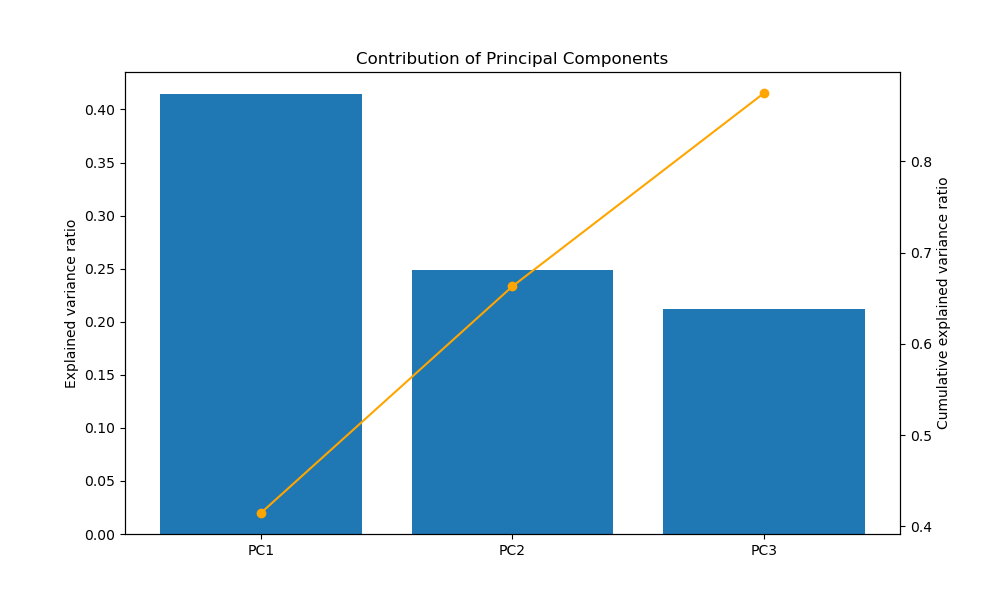
\includegraphics[scale=0.2]{Chapter-3/Figures/contribution.png}  %以pic.jpg的0.5倍大小输出
%         \end{minipage}
%     }
%     \subfigure[Line]{ %第二张子图
%         \begin{minipage}{7cm}
%             \centering    %子图居中
%             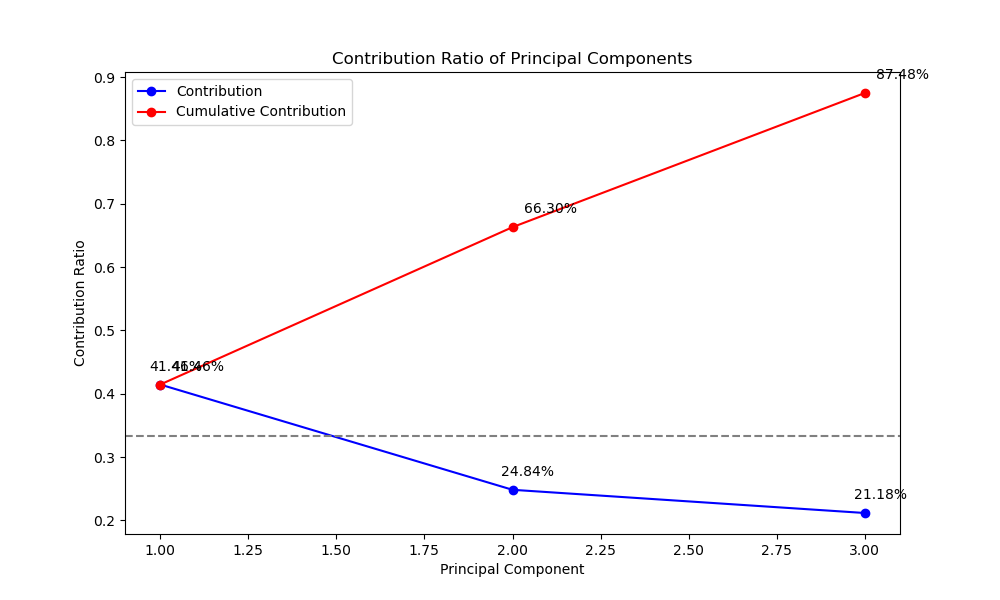
\includegraphics[scale=0.2]{Chapter-3/Figures/contribution2.png}%以pic.jpg的0.5倍大小输出
%         \end{minipage}
%     }
%     \caption[Principle Components Contribution]{Principle Components Contribution}    %大图名称
%     \label{principlecomponentcontribution}    %图片引用标记
% \end{figure}

Consequently, Principal Components Analysis (PCA) was employed to reduce the data into two and three dimensions separately. By retaining the two and three principal components with the highest information content, it became feasible to compare the characteristics between jurisdictions.

The results of the PCA variance analysis reveals that the first two components capture 67\% of the information, and the first three components capture 87\% of the information. Given this, we employed PCA to reduce data into two and three dimensions, respectively. By retaining the principal components with the highest information content, we were able to compare the
characteristics between jurisdictions, using scatter plot diagrams (see Figure \ref{Figure 2.2}). In both the two-dimensional and three-dimensional scatter plot diagrams, the red, blue, and green points exhibit distinct distributions, with each color forming its own cluster.
% \begin{figure}[H]
%     \centering  %居中
%     \subfigure[Histgram]{   %第一张子图
%         \begin{minipage}{7cm}
%             \centering    %子图居中
%             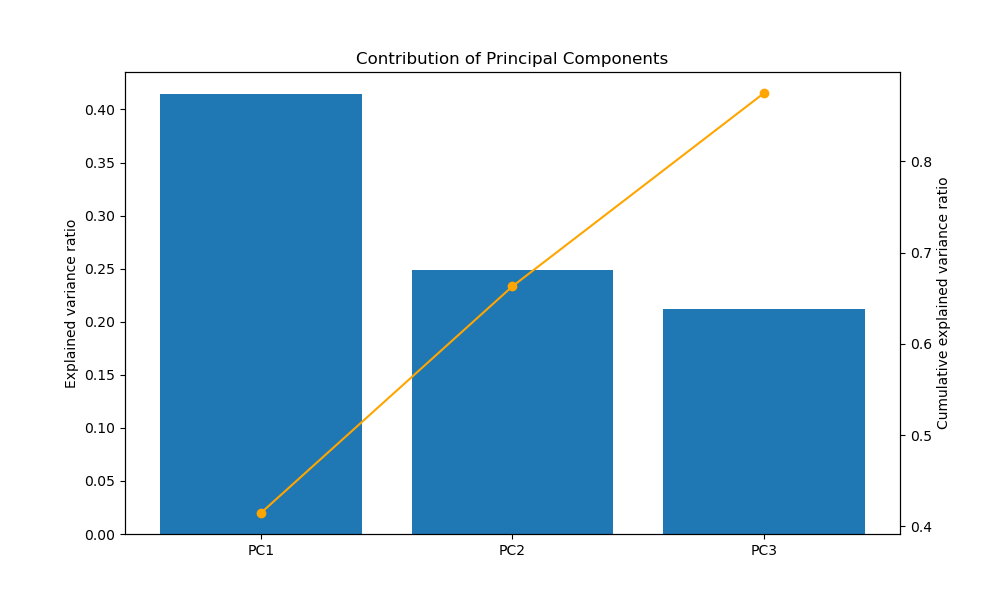
\includegraphics[scale=0.2]{Chapter-3/Figures/contribution.png}  %以pic.jpg的0.5倍大小输出
%         \end{minipage}
%     }
%     \subfigure[Line]{ %第二张子图
%         \begin{minipage}{7cm}
%             \centering    %子图居中
%             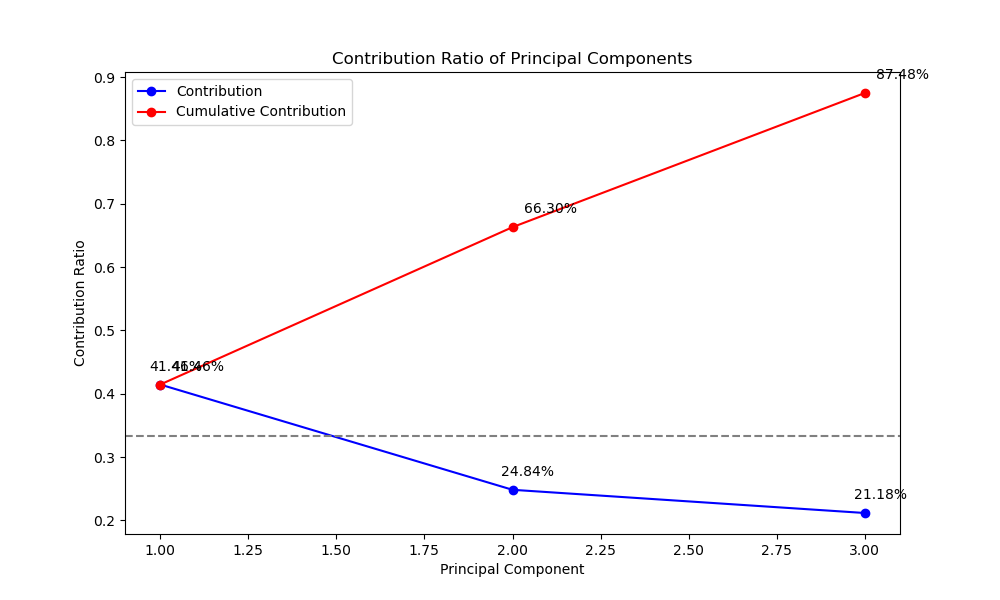
\includegraphics[scale=0.2]{Chapter-3/Figures/contribution2.png}%以pic.jpg的0.5倍大小输出
%         \end{minipage}
%     }
%     \caption[Principle Components Contribution]{Principle Components Contribution}    %大图名称
%     \label{principlecomponentcontribution}    %图片引用标记
% \end{figure}
Although the reduced components lack specific economic meaning, it is notable that many state characteristics exhibit a cluster distribution. Both the two-dimensional and three three-dimensional scatter plot diagrams suggests that states governed by the same political party share similar economic and social characteristics. This is notably different from states governed by other parties. In summary, therefore, the PCA indicate a high level of cohesion within states governed by the same party in terms of their economic and social characteristics, while significant differences exist between states governed by different parties. This finding is consistent with \Textcite{martin2018dividing}'s proposition that jurisdictions with similar features may have winners emerging from the bargaining game that are free riders, thereby predicting the outflow of funds from the winning coalition.

The scatter plot diagrams also show that republican states, democratic states, and swing states exhibit distinct cluster distributions in their respective areas. In the 2D plot presented, red and blue dots are situated on opposing sides, with swing states occupying the intermediary position. This
configuration implies that any modifications to the grant formula favoring one party inflicts significant harm to the other. This observation may reflect opposition between the two parties during legislative bargaining, while swing states remain relatively indifferent. The distinctive nature of swing states is further highlighted in the 3D scatter plot, where green dots do not align. While it may not be surprising that traditional Republican states share similar social characteristics, the 3D scatter plot provides an alternative perspective on fiscal collective behavior within the Republican party. It raises the question of whether those who take part in the bargaining process act based on
their political status or advocate for the benefits of the jurisdiction they represent. Hence, the preference effect may be mixed with the “free-rider” effect. To evaluate the effect of party preference, alignment and structure of different branches, the "free rider" effect should be carefully controlled.

In summary, the apparent collective alliance among ostensibly similar political parties may be the result from the similarities in economic and social characteristics of states governed by the same political party. Hence, the PCA results underscores the need to establish a micro-foundation for any
collective political behavior within a party. That is, it is essential to analyze the motivations of individual members rather than attributing it to collective group behavior.

\subsection{Step 2: Fixed Effect Regression Analysis}

To test the above four hypotheses, we employed a fixed effect regression analysis, a method ideally suited for panel data where multiple observations from the same entities (in this case, states) are observed over time. This approach allows us to control for unobserved heterogeneity that could bias our results, meaning it accounts for inherent characteristics of each state that do not change over time or are constant for each state across the study period. By focusing on the variations within each state, rather than between states, fixed effect models provide a more accurate estimation of the impact of political alignment and party preference on IGT distributions.

In preparation for the fixed effect regression analysis, we structured our panel dataset to include state-specific observations across multiple years, capturing the annual total amounts of IGT received by each state, along with the political party alignments at both the state and federal levels.
The model included dummy variables for each state to capture unobserved, time-invariant characteristics. Independent variables of interest were lagged to address potential endogeneity concerns, ensuring that we capture the effect of prior political conditions on current IGT distributions. The regression equation was also augmented with time dummies to control for year-specific
effects that might influence all states similarly, such as national economic conditions or federal policy changes. Standard errors were clustered at the state level to account for serial correlation within states over time. This comprehensive approach allowed us to examine the above hypotheses, while controlling for both observed and unobserved factors that could skew the results.


\subsubsection{Data and Variables for Regression}

Similar to the PCA, stratified sampling is also adopted. The sample states used when conducting the regression analysis are therefore the same as the ones used for the PCA. These were grouped into traditional Republican states, traditional Democratic states, and swing states. The dependent variable in the regression model is the annual total IGT amount received by state $i$. This variable
was operationalized though logarithmic transformation.

The independent variables include $c$, which is a dummy variable that represents alignment combination and $p$, which represent partisanship. More specifically, the dummy variable $c$ represents the party distribution combination in the administrative and legislative branches across
federal and state levels. Three key factors determine the nature of $c$: the governmental level, branch, and part. As depicted in Table \ref{Table 2.6},these factors can be presented in a $2\times2$ table with two
branches and two levels, resulting in four sectors. These sectors are denoted as $u_1, u_2, s_1, s_2$. Each sector has two possible parties in control, namely the Democratic party "$d$" and the Republican party "$r$".
% \end{table}%

In this study, the majority in the House of Representatives defines the partisan composition of the legislative branch, given its pivotal role in the budget-making process. The partisan composition of the administrative branch is determined by the partisan affiliation of the administrative leader, who
could be the president or governor. There are 16 combinations in $c$:

$$(r, r, r, r), (r, r, r, d), (r, r, d, r), (r, r, d, d), (r, d, r, r), (r, d, r, d), (r, d, d, r), (r, d, d, d)$$\\$$(d, r, r, r), (d, r, r, d), (d, r, d, r), (d, r, d, d), (d, d, r, r), (d, d, r, d), (d, d, d, r), (d, d, d, d) $$

We employ $c_1, c_2, . . . c_{16}$ to denote the 16 distinct combinations. In the regression analysis, only fifteen combinations are retained, with the omission of the first combination $c_1 = (r, r, r, r)$ to mitigate multicollinearity issues. $c_1$ serves as the benchmark in the regression model.


In the regression analysis, I incorporate a 1-time period lag of $c$ as an independent variable. The rationale behind this is that the general decision-making process is time-consuming, implying that the effect of a specific party combination $c$ should not be significant in the current year.

Regarding the dummy variable $p$, we gathered longitudinal data for three distinct types of states based on their political affiliations, including traditional Democratic states, Republican states, and
swing states. The 14 states are categorized into three groups. The first group constitutes the traditional Republican states, often referred to as the “red wall states.” We refer to this group as $p = 1$ The second group (referred to as $p = 2$) comprises traditional Democratic states, also known as
the “blue wall states.”. The third group (referred to as $p = 3$) represents swing states, commonly referred to as the “battleground states.”

The control variables encompass prevalent social and economic factors integrated into the distribution formula for federal grants projects. These factors, identified in the literature, can be inferred to have an impact on grants distribution and variables included can be listed in Table \ref{Table 2.5}. The variables that are included in the analysis covers the period from 2000 to 2019.

With panel data spanning 19 years, we adopt a fixed effect model approach to overcome potential omitted variables. In total, we develop and test the above hypotheses through three regression models. The benchmark model is an Ordinary Least Squares (OLS) regression with robust standard error. The second model is a time factor and individual factor fixed regression. The third model is
an individual variable fixed model. The equations for these three models are as follows:

Model 1 - OLS Regression:

\begin{equation}
    \begin{split}
        log(igt_{i,t}) & = \alpha + \beta_1 c_{i,t-1} + \beta_2 p_{i,t} + \beta_3 log(gdp) + \beta_4 log(pl) + \beta_5 log(mhi_{i,t}) \\
        & + \beta_6 wapw_{i,t} + \beta_7 ur_{i,t} +\beta_8 log(prm_{i,t}) + \epsilon_{i,t}
    \end{split}
\end{equation}
$For\ t = 1, 2, 3...T\ and\ i = 1, 2, 3...N $

Model 2 - Fixed effect model with time and state fixed:
\begin{equation}
    \begin{split}
        log(igt_{i,t}) & = \alpha_i + \theta_t + \beta_1 c_{i,t-1} + \beta_2 p_{i,t} + \beta_3 log(gdp) + \beta_4 log(pl) + \beta_5 log(mhi_{i,t}) \\
        &+ \beta_6 wapw_{i,t} + \beta_7 ur_{i,t} +\beta_8 log(prm_{i,t}) + \epsilon_{i,t}
    \end{split}
\end{equation}
$For\ t = 1, 2, 3...T\ and\ i = 1, 2, 3...N $

Model 3 - Fixed effect model with state partisanship controlled:

\begin{equation}
    \begin{split}
        log(igt_{i,t}) & = \alpha_i + \beta_1 c_{i,t-1} + \beta_2 p_{i,t} + \beta_3 log(gdp) + \beta_4 log(pl) + \beta_5 log(mhi_{i,t}) \\
        &+ \beta_6 wapw_{i,t} + \beta_7 ur_{i,t} +\beta_8 log(prm_{i,t}) + \epsilon_{i,t}
    \end{split}
\end{equation}
$For\ i = 0,1,2...N$.

%%%%%%%%chatgpt checked%%%%%%%%%%%%


\section{Results}

% Principal Components Analysis (PCA) was employed to reduce the data into two and three dimensions separately.The resulting scatter plot following data dimension reduction is presented in Figure \ref{Figure 2.2}.

% % \begin{figure}[H]
% %     \centering  %居中
% %     \subfigure[2 Principle Components Analysis Scatter]{   %第一张子图
% %         \begin{minipage}{7cm}
% %             \centering    %子图居中
% %             \includegraphics[scale=0.45]{Chapter-3/Figures/pca.png}  %以pic.jpg的0.5倍大小输出
% %         \end{minipage}
% %     }
% %     \subfigure[3 principle Components Analysis Scatter]{ %第二张子图
% %         \begin{minipage}{7cm}
% %             \centering    %子图居中
% %             \includegraphics[scale=0.45]{Chapter-3/Figures/pca_3d.png}%以pic.jpg的0.5倍大小输出
% %         \end{minipage}
% %     }
% %     \caption[Principle Components Analysis Scatter Plot]{Social Characteristics Principle Components Analysis Scatter Plot}    %大图名称
% %     \label{Figure 2.2}    %图片引用标记
% % \end{figure}
% %%chatgpt checked%%%%%

% Although the reduced dimensions lack specific economic meaning, a notable observation in Figure \ref{Figure 2.2} is that many state characteristics exhibit a cluster distribution. In both two-dimensional and three-dimensional plots, the red, blue, and green points exhibit distinct distributions, with each color forming its own cluster. This suggests that states governed by the same political party share similar economic and social characteristics, which are notably different from those of states governed by other parties. In summary, principal component analysis results indicate a high level of cohesion within states governed by the same party in terms of their economic and social characteristics, while significant differentiation exists between states governed by different parties.

% Such findings align with \Textcite{martin2018dividing}'s proposition that jurisdictions with similar features with winner players in the bargaining game may act as free riders, consequently predicting the outflow of funds from the winning coalition.

% Another potential implication arises from the hierarchical distribution based on political parties. Republican states, Democratic states, and swing states exhibit distinct cluster distributions in their respective areas. In the 2D plot presented in Figure \ref{Figure 2.2} (a), red and blue dots are situated on opposing sides, with swing states occupying the intermediary position. This configuration implies that any modification to the grants formula favoring one party inflicts significant harm on another. This observation may elucidate the sharp opposition between the two parties during legislative bargaining, while swing states remain relatively indifferent. The distinctive nature of swing states is further illuminated in the 3D plot depicted in Figure \ref{Figure 2.2} (b), where green dots do not align on the same plane in the third dimension.

% While it is unsurprising that traditional Republican states share similar social characteristics, this figure provides an alternative perspective on any fiscal collective behavior within the party. It prompts consideration of whether members in the bargaining process act based on their political status or advocate for the benefits of their represented jurisdiction. Therefore, the effect of different party preference, alignment between federal and state are mixed with the "free-rider" effect. To evaluate the effect of party preference, alignment and structure of different branches, the "free rider" effect should be carefully controlled.

% PCA result underscores the need to establish a micro-foundation for any collective political behavior within a party. In other words, it is essential to analyze the motivations of individual members rather than attributing the behavior purely as group behavior. In the case of intergovernmental transfer, the apparent collective alliance among ostensibly similar political parties may, in reality, result from the similarity of economic and social characteristics within states governed by the same political party.

%%%%%%%%chatgpt checked%%%%%%%%%%%%


% \subsection{Regression Results and Analysis}
The regression results generated show that while all three models developed for this study exhibit high adjusted R-square values (0.835,0.855,0.791 separately) and the second model is superior to the other two models. It exhibits the highest adjusted R-square value. Moreover, with two factors
fixed, it allows us to better control for omitted variables, which makes the significance of the coefficients more convincing. Given this, the subsequent analysis centers on the results generated from model 2 (see Table \ref{Table 2.7}, \ref{Table 2.8} and \ref{Table 2.9}).

%%%%%%%chatgpt checked%%%%%%%%%%%%

In model 2, seven coefficients are statistically significant at 5\% significance level, including $c_2(0.00246), c_3(-0.00751), c_5(-0.0163),c_6(0.0119), c_{11}(.00893), c_{13}(0.00919), c_{15}(-0.00713)$. In addition, the partisan variables “Democratic States” and “Swing States” are statistically significant.
%%%%%chatgpt checked%%%%%%%%%%%%

The regression results support the hypothesis concerning unified government. That is, that a unified federal government is positively associated with higher overall IGT spending. A comparison of the coefficients of $c_5(r, d, r, r)$ and $c_1(r, r, r, r)$ reveals that a traditional Republican state, where both the administrative and legislative branches are controlled by the Republican party, experiences a 1.63\% reduction in intergovernmental transfers proportion under bipartisan control at the federal level compared to a
situation where the federal government is uniformly controlled by the republican party. This suggests that the federal government' ability to distribute grants to states level is significantly constrained when the Republican party is not unified at the federal level.
%%%chatgpt checked%%%%%


As noted earlier, the coefficient of $c_{16}$ in second model is deleted to overcome the multicollinearity problem. As such, we had to rely on the results generated from Model 1 and Model 3 when analyzing the second hypothesis. That, the hypothesis that political party color is related to the level of IGT spending.  A comparison of $c_{16}(-0.006)$ and $c_1(0)$, suggest that states
receive a 0.6\% lower intergovernmental transfer when both the federal and state levels are controlled by the Democratic party, in contrast to a scenario where both levels are under Republican control. This suggest that a republican party preference is present for allocating more resources to state governments. However, $c16$ is not significant (t= -1.65) thus we cannot reject the null
hypothesis that there is no difference between $c1$ and $c16$. Hence, the second hypothesis is not supported by our analysis.

%%%chatgpt checked%%%%%

The third hypothesis tested is that the level of political party alignment across the federal and state governments is positively related to IGT distributions. Our analysis offers statistically significant support for this hypothesis. When comparing the aligned combination $c_1(r, r, r, r)$ and $c_3(r, r, d, r)$, the negative coefficient of $c_3$ indicates that unaligned states with a Republican-controlled federal government would receive fewer grants. Specifically, aligned Republican states receive 0.75\% more grants compared to states with a Democratic governor. Another example of the alignment effect is the negative coefficient of $c_{15}$, which indicates that when a republic governor facing a democratic federal government, state government would receive 0.7\% less in grants funds.

The final hypothesis tested is that battle ground (i.e., swing states) states are more likely to secure IGTs compared to non-battle ground states. Swing states receive significantly less in grant funding, compared to non-swing states. This contradicts hypothesis 4. One potential explanation is that,
while swing states are crucial in determining election outcomes during election years, in nonelection years, the federal government may be reluctant to allocate additional resources to states controlled by opposing parties. The characteristics of swing states may lead the federal government
to believe that it is not meaningful to appease swing states in non-election years.

In summary, the PCA analysis underscore the role of social and economic underpinnings in the unintended distribution of grants. Nevertheless, when the most impactful social and economic variables are controlled for in the two-factor fixed regression, two of the four hypotheses are supported, reaffirming the substantial influence of political party affiliations on grant allocations.



\section{Review and Summary}

This research examined the role of political party control in the distribution of intergovernmental transfers (IGTs) in the United States. Toward this end, we analyzed a panel data set spanning 19 years, using both PCA and fixed-effect regression models. The combination of these two methodological approaches allowed us to investigate the impact of political alignments on IGTs at
both the state and federal levels, while controlling for relevant socio-economic factors. The analysis indicates that political congruence between state and federal governments plays a significant role in determining the flow of intergovernmental funds, with states aligned with the federal ruling party receiving favorable IGT allocations. This finding suggests that IGT allocation decision includes a strategic political dimension that transcends beyond mere economic and social needs.

The study is endowed with some limitation that needs to be considered when interpreting the data used in this study. These arise primarily as a result of the difficulties involved in gaining access to and collecting the data used in the study. One such limitation is the limited time span of the data used in the study (19 years), which may reduce the robustness of our model. A second limitation arises from the fact that we employed the total amounts of IGTs received by states as dependent variables. As such, we were unable to distinguish between competitive grants and formula grants in the regression. This limitation may lead to some aggregation problems. For instance, the free rider effect may not be significant in competitive grants. Despite of these limitations, the study makes several contributions. First, it adds to an area of research that has received very limited attention--the role of political party control in IGTs. Perhaps most important, this study adds to this limited
body of research by illuminating the intricate relationship between political affiliations and IGT distributions, highlighting the important role that political considerations may play in this process.


Another important contribution of this study is that it may also serve to inform prior research findings discourse related to the so-called flypaper effect. The flypaper effect posits that an increase in grants-in-aid lead to significantly higher public spending compared to the same increase in
private income, causing funds to “stick where they hit” \parencite{inman2008flypaper}. Scholars attribute this phenomenon to various causes. Hamilton, for instance, attempted to explain the flypaper effect as a result of improper data distinction or empirical methods \parencite{hamilton1986flypaper}, while others associate the flypaper effect with fiscal illusion \parencite{gramlich1997stimulative}.This research may be viewed as a novel perspective to explain the flypaper effect. The confirmed political factor impact during IGT distribution suggests that: for certain states, obtaining grants from the federal government is easier
compared to generating revenue through other means. This relative price effect may explain the inclination of state governments to prefer raising funds from IGTs rather than through taxation. Following this logic, the magnitude of the flypaper effect should be influenced by the partisan distribution between the central and state governments. States that are prone to free-riding or are
favored by a central government may experience a greater flypaper effect, as grants for such subnational entities are relatively easier to obtain, amplifying their spending tendencies.
    % !TEX root = ../YourName-Dissertation.tex

\chapter{Effect of Intergovernmental Transfer on Local Governments' Spending Behavior}

Chapter 4 marks a pivotal transition in our exploration of fiscal federalism, shifting the lens to the specific impacts of transfer payments on local government fiscal behavior, including public spending actions and revenue collection behaviors. Prior to delving into the core analysis, it is imperative to contextualize our investigation within the existing scholarly landscape. The literature on transfer payments' effects is rich and diverse, generally bifurcated into studies examining inter-jurisdictional impacts and those focusing on the fiscal behavior of local governments themselves, summarized as Figure \ref*{Figure 3.1}. The top side of Figure \ref{Figure 3.1} focuses on the topic of transfer payments' impacts across regions, while the lower side concentrates on the effects on subnational governments' own fiscal behaviors, which are further divided into fiscal expenditure behavior and fiscal revenue behavior. For example, the topic across regions may include: the role of transfer payments in influencing revenue equity and their role in enhancing fiscal equity across regions. This latter category, which forms the crux of Chapters 4 and 5, is further divided based on the nature of fiscal behavior under examination: public spending (Chapter 4) and tax collection activities (Chapter 5).

Chapter 4 of this dissertation critically examines the impact of intergovernmental transfers on the spending behavior of local governments, specifically through the lens of the "flypaper effect." This analysis is pivotal to the dissertation's overarching goal of delineating the intricate web of fiscal interactions and their implications within the fiscal federalism framework. By systematically reviewing the literature and employing a mathematical model to investigate how these transfers influence local expenditure decisions, this chapter contributes to a deeper understanding of the behavioral dynamics at play within fiscal federalism. It highlights the nuanced ways in which federal grants affect local spending priorities and practices, thus providing essential insights into the efficiency and effectiveness of resource allocation across government tiers. This exploration not only enriches our theoretical knowledge of fiscal federalism but also offers practical guidance for policymakers aiming to optimize public goods provision through strategic intergovernmental transfers. Consequently, the findings and discussions presented in this chapter enhance the comprehensive analysis of fiscal strategies explored throughout the dissertation, reaffirming the significance of understanding fiscal behaviors in achieving equitable and efficient public service delivery.

In Chapter 4, I conduct a comprehensive review of literature related to the effect of intergovernmental transfer on subnational government spending, with a key focus on systematically categorizing explanations for the flypaper effect observed in previous studies. Recognizing a gradual deepening in scholars' understanding of the flypaper effect, we divide this evolution into three stages. In addition, by developing and refining a model to simulate the specific causes behind the flypaper effect, we offer a mathematical representation that allows for its visualization, enabling an intuitive observation of changes in the effect's magnitude.

\section{Fungibility and Flypaper Effect}

One intuitive philosophy about the effect of IGT on subnational government spending is called "fungibility" \parencite{pack1993foreign}, which means the intergovernmental transfer received by local government would substitute the local government's revenue. Recipients assimilate federal funds into general revenue and reduce the spending on public goods through a reduction of local taxes within the jurisdiction. However, supportive empirical evidence are quite limited. On the contrary, evidence on flypaper effect is widespread everywhere.

The flypaper effect is widely regarded as the most influential phenomenon in the fiscal federalism literature regarding the vertical transfer of funds from the federal to the state or local level \parencite{hines1995anomalies,gamkhar2007impact}. According to Bradford and Oates' model, a lump sum grant to the state or local level should have the same effect as an increase in individual revenue within the jurisdiction in terms of stimulating public expenditure \parencite{bradford1971analysis}. This conclusion is known as the equivalence theorem, which is based on two fundamental assumptions: the median voter theorem and lump-sum tax collection by federal, state, and local governments. However, empirical evidence does not support this theorem. Specifically, some researchers have found that a \$1 increase in individual revenue leads to an increase in public expenditure of only \$0.02 to \$0.05, while a \$1 increase in intergovernmental transfers can lead to an increase in public expenditure of \$0.25 to even \$1 \parencite{bailey1998flypaper,dollery1996empirical,gamkhar2007impact}. This phenomenon is known as the flypaper effect. According to Inman's statistics, over 3,500 research papers have investigated the flypaper effect, both theoretically and empirically \parencite{inman2008flypaper}.

In this section, I'm summarizing how scholars in different stages explain the flypaper effect. The understanding of flypaper effect went through a incremental progress, though may not be chronologically. This progress can be identified as three phrases. In the first stage, the conventional analysis, scholars believe the matching grants have both price effect and income effects while the non-matching grants is analogous to the lump-sum subsidy, which means only income effects exists. In second stage, some scholars start to realize that non-matching grants has price effects as well, but that's due to the impact of fiscal federalism setting and fiscal illusion. Federal government collecting revenue then redistributing to state and local generates fiscal illusion since this process is too complicated for consumers to perceive. In third stage, scholars start to realize the effect of distortionary tax that collect by grants recipient. The distortionary tax policy together with the low administrative efficiency in state and local leads to a higher marginal cost of the tax collection. Hence no matter the grants is matching or non-matching, the state or local government trend to use the grants rather than the tax revenue to cover the expenditure.

The investigation on flypaper effect in my view can be divided into 3 phrase from the shallower to the deeper.

\section{Literature on Flypaper Effect}
\subsection{Phrase One}

Except for the introduction of intergovernmental transfer in figure \ref*{grantstype}, one important concern about IGT in economic analysis is the matching mechanism. For matching grants, federal governments will reimburse a specific ratio for each 1 dollar of state and local expenditure. Based on whether federal government set a cap on the matching grants, matching grants can be divided into open-ended matching grants and closed-ended grants.
%%%%%%%%%%%%%%%%%%%%%%%%%%%%%%%%%%%%%%%%%%%%%%%%%%%%%%%%%%%%%%%%%%%%%%%%%%%%%
%%%%%%%%
As is shown in figure \ref{Figure 3.3}, the two parallel lines $L1$ and $L3$ are budget constraint of the economy before and after the non-matching grants and $L3$ is the budget constraint with matching grants which is the red line. The difference between $G_m$ and $G*$ is the combination of price effect and income effect of matching grants.

The matching grants model explains why scholars in first stage explain the fly paper effect by misspecification or omitted variable. Misspecification refers to instances where researchers may conflate matching grants with lump-sum grants, leading to a mix-up of price effects and subsequently resulting in increased public goods spending \parencite{lankford1987note,henderson1968local}. Matching grants reduce the marginal price of public services, thus mix-up with lump-sum grants would lead to an increase in public goods spending \parencite{gramlich1997state}. Some scholars attribute the flypaper effect to omitted variables or pre-selection issues. \textcite{knight2002endogenous} developed a two-level bargaining model to demonstrate that the federal government distributes intergovernmental transfers to states and local governments with a higher propensity to spend, indicating that the flypaper effect is not a result of intergovernmental transfers. However, prior studies and investigations have encountered endogeneity issues. To address this, Knight conducted an empirical test where he employed an instrumental variable to control for the endogeneity problem. His results indicate that once the pre-selection issue is filtered out, the flypaper effect is not evident, at least for the data he collected regarding interstate highway programs. To summarize, the understanding under this view is that the flypaper effect may not actually exist, but may instead be a result of misspecification or omitted variables.

\subsection{Phrase two}

The literature on the flypaper effect has also been approached from a second perspective, whereby scholars recognize the importance of lump-sum grants and their potential price effects. While scholars in the first stage focused on the price effects of matching grants, it was realized that this may not be sufficient to explain the large gap in the flypaper effect. As such, the second stage of literature argues that non-matching grants also have price effects, which can be attributed to fiscal illusions. \textcite{mcculloch1845treatise} argued that taxpayers often misperceive the costs of governmental activities, a concept later summarized as fiscal illusions. The theory of fiscal illusion was first developed by Italian economist \textcite{puviani1903teoria}in his 1903 book \textit{Teoria della illusione finanziaria}. \textcite{wagner1976revenue} introduced this concept in America and identified the effect of fiscal illusions on local government spending. \textcite{oates1979lump,borge1995lump} also recognized the potential price effect of non-matching grants and attempted to explain it using the concept of fiscal illusions. The lower-estimated public good price generates a even flatter slope of the budget constraint compared to the $L_3$ in figure \ref{Figure 3.3}.

The existence of fiscal illusion can be attributed to administrative factors and institutional intention. The fiscal federalism framework is complex and difficult for residents to comprehend, while administrative processes are often opaque and lack transparency, preventing residents from understanding the nuances of intergovernmental grants and their own contributions to these grants. Empirical research by \textcite{turnbull1998overspending} supports this view, demonstrating that imperfect information generates a broader fiscal illusion based on municipal data. Additionally, the budget-maximizing tendencies of bureaucratic systems are supported by both empirical evidence and theoretical inference \parencite{mueller2003public,brennan1977towards}. This tendency is sometimes referred to as "Leviathan government," in which governments seek to maximize their budgets rather than prioritize residents' utility \parencite{quigley1986budget}. The combination of budget-maximizing bureaucrats and lower perceived prices of public goods leads to increased expenditure on public goods.


\subsection{Phrase Three}

In stage three, Scholars have also examined the effect of the cost of tax collection within a jurisdiction. This cost can arise from two aspects, one being the distortionary tax, another one comes from the revenue collection ability of the sunational government. Assuming that tax revenue collection does not cause any distortion for the recipient is a strong assumption. In reality, changes in state and local government tax policies can significantly alter residents' behavior. For instance, if residents are dissatisfied with tax and public goods policies, they may choose to work less and spend more time on leisure. Alternatively, they may move to another jurisdiction, which itself incurs costs due to the tax increase. \textcite{hamilton1986flypaper} was the first to observe that the cost of tax collection within a jurisdiction leads to a curved budget constraint, rather than a straight line. However, his idea was not widely accepted at the time, and he neglected to consider administrative ability as a source of cost, focusing only on deadweight loss as the source of tax collecting cost.


In reality, the cost of tax collection comes from various sources, including the different levels of administrative ability between federal and state governments. \textcite{volden2007intergovernmental} developed a game theory model to simulate the interaction between the federal government and lower-level governments and showed that the different costs of collecting revenue for federal and state governments partially explains the flypaper effect. \textcite{dahlby2016stimulative} argued that the price effect of non-matching grants exists even without fiscal illusion due to subnational governments face information and ability disadvantages, meanwhile \textcite{vegh2016unsticking} came to a similar conclusion. In summary, these researchers suggest that the collection of tax revenue is costly for state and local governments due to factors such as administrative inefficiency and distortion, leading to a preference for using "cheaper" resources such as intergovernmental transfers. Therefore, even non-matching grants or lump-sum grants can have price effects.

Some horizontal government interaction explains this distortion as well, \textcite{brueckner2003strategic} develops a strategic model to analyze the state and local fiscal behavior, he concludes that the lower-level governments are quite sensitive to other competitors. This sensitivity may explain why state and local government don't want tax increase revenue to cover the public goods. Other horizontal interaction theory such as yardstick competition or tax competition also explains the sensitivity.



I expand the benchmark model by introducing the distortion of tax collection into it.


\section{Mathematical Expression of Flypaper effect}

Following the comprehensive literature review on the flypaper effect, the next step involves developing a mathematical model to simulate this phenomenon. Beginning with foundational assumptions where the flypaper effect is initially absent, the model progressively incorporates a variety of taxes and refines utility functions to provide a clear and explicit explanation of the reasons behind the flypaper effect. This approach aims to elucidate the underlying mechanics of the effect, offering a theoretical framework that enhances our understanding through a step-by-step augmentation of model complexity.

\subsection{Benchmark model}

The Benchmark model is similar to \Textcite{vegh2016unsticking}'s benchmark model with small modification.

To make the benchmark model as straight forward as possible while capture the IGT mechanism. I assume that:

\begin{enumerate}
    \item Economy is static.
    \item Only one local government and representative citizen in this economy.
    \item Two kinds of goods in the economy which are public good $G$ \label{G} and private good $X$.\label{X}
    \item Resident spend all there income $y$, which is given, on either private goods $X$ or tax $\tau$.\label{y}
    \item The tax is lump-sum tax with no dissertation.
    \item Source of government revenue: tax $\tau$ and transfer $f$.\label{f}
    \item Type of transfer: Nonmatching grants,like lump-sum subsidy.
\end{enumerate}

The representative citizen's budget constraint is:
\begin{equation}
    y=X+\tau \label{bmrc budgetc}
\end{equation}
The local government's budget constraint is:
\begin{equation}
    f+\tau=G \label{bmlg budgetc}
\end{equation}
Combine equation \ref{bmrc budgetc} and \ref{bmlg budgetc}, I get a budget constraint for the economy:
\begin{equation}
    y+f=X+G \label{bmecoconstrain}
\end{equation}

The utility for representative resident comes from the utility of $X$ and $G$. I assume the utility function is the Cobb-Douglas form thus it's a concave utility:

\begin{equation}
    U(X,G)=AX^{\alpha}G^{1-\alpha} , 0<\alpha<1 \label{bmrcutility}
\end{equation}

For the representative resident, the problem is to choose proper level of $X$ to maximize the utility in equation \ref{bmrcutility} subject to equation \ref{bmrc budgetc}. The Lagrangian equation can be set up as:

\begin{equation}
    L(X)=AX^{\alpha}G^{1-\alpha}+\lambda_{rc}(y-X-\tau)  \label{bmrclagrangian}
\end{equation}

Solving the equation \ref{bmrclagrangian} will get first order condition(foc):

\begin{equation}
    \alpha A\left(\frac{X}{G}\right)^{\alpha-1}=\lambda_{r c} \label{lamdarc}
\end{equation}

\begin{equation}
    y=X+\tau \label{rcfoc}
\end{equation}

To solve the Ramsey problem, the Ramsey planner needs to decide the level of $X,G$ to maximize the utility subject to equation \ref{bmecoconstrain} and equation \ref{bmlg budgetc}. The Lagrangian can be set as:

\begin{equation}
    L(X,G)=AX^{\alpha}G^{1-\alpha}+\lambda_{e}(y+f-X-G)+\lambda_{lg}(f+\tau-G)  \label{bmeclagrangian}
\end{equation}

Solving the equation \ref{bmeclagrangian} will generate:

\begin{equation}
    \alpha A\left(\frac{X}{G}\right)^{\alpha-1}=\lambda_e+\lambda_{l g}
    \label{foc on X}
\end{equation}

\begin{equation}
    (1- \alpha) A\left(\frac{X}{G}\right)^{\alpha}=\lambda_e+\lambda_{l g} \label{foc on G}
\end{equation}

\begin{equation}
    y+f=X+G \label{foc on lambdae}
\end{equation}

\begin{equation}
    f+\tau=G \label{foc on lambdalg}
\end{equation}

Combining equation \ref{foc on X}, \ref{foc on G}, \ref{foc on lambdae} will generate:

\begin{equation}
    (1-\alpha)y+(1-\alpha)f=G \label{bmresult}
\end{equation}

The flypaper effect definition can be mathematically expressed as $\frac{d G}{d f}-\frac{d G}{d y}$. Given equation \ref{bmresult}, the flypaper effect $fe=0$, which means, under this setting, theoretically there should be no flypaper effect.

\subsection{Ramsey Model with Distortionary Tax Collection}

To capture the distortion effect of the tax,I loosen the 3rd and 5th assumption of the benchmark model. I follow the setting by \textcite{vegh2016unsticking} by adding a taxable private goods $X_t$ to differentiate with the non-taxable private goods $X_{nt}$ and capture the distortion effect of proportional tax. In reality, $X_{nt}$ could express any behavior that representative resident take to avoid the taxation, such as more time on leisure or
The assumption on taxation and representative resident's spending behavior are:

\begin{enumerate}
    \item Three kinds of goods in the economy which are public good $G$ and taxable private good $X_t$ and non-taxable private good $X_{nt}$.\label{Xt}
    \item Resident spend all there income $y$, which is given, on either taxable private goods $X_t$, non-taxable private goods $X_{nt}$ or tax.
    \item The tax is proportionary tax on $X_{t}$, with tax rate $\theta$.
\end{enumerate}

So the budget constrain for resident, local government and the whole economy could be separately list as:

\begin{equation} \label{distortionrct}
    y=X_t(1+\theta)+X_{n t}
\end{equation}
\begin{equation} \label{distortiongct}
    f+\theta X_t=G
\end{equation}
\begin{equation} \label{distortionect}
    y+f=x_t+x_{nt}+G
\end{equation}

Different from Carlos' setting who accept a more general setting on residents' and governments' utility, I set Cobb-Douglas form on utility to get a arithmetic solution. Unlike the benchmark model in Carlos' research, in which he set the linear utility, the Cobb-Douglas setting means the imperfect substitute between private and public goods, which is a more reasonable setting. The distribution on $X_t$, $X_{nt}$ and $G$ should maximize representative resident's utility and government's utility.

\begin{equation} \label{rclgutility}
    \left\{\begin{array}{l}U=A X^\alpha G^{1-\alpha} \\ X=B X_t^\beta X_{n t}^{1-\beta}\end{array}\right.
\end{equation}
Where X represent a compound private good.

For resident, they need to decide $X_t, X_{nt}$ to maximize $U$ subject to equation \ref{distortionrct}. For local government, the problem is to decide the distribute of $X$ and $G$ to maximize $U$, thus the Ramsey problem is to maximize both resident and local governments' utility, which is listed as equation \ref*{rclgutility} subject to equation \ref{distortionrct} and \ref{distortiongct}. For resident, the first order conditions on $X_t, X_{nt}, \lambda_{rc}$ can be listed as:

\begin{align}
    \begin{split}
        \frac{\partial U}{\partial X} \frac{\partial X}{\partial X_t}=(1+\theta) \lambda_{r c} \label{focxt}
    \end{split}                     \\
    \begin{split}
        \frac{\partial U}{\partial X} \frac{\partial X}{\partial X_{nt}}=\lambda_{r c} \label{focxnt}
    \end{split} \\
    \begin{split}
        y=X_t(1+\theta)+X_{nt} \label{foclabrc}
    \end{split}
\end{align}

Solving equation \ref{focxt}, \ref{focxnt} will generate the relationship between $X_t$ and $X_{nt}$ in equilibrium and the level of $\theta$:

\begin{align}
    \begin{split}
        X_{nt}=\frac{(1-\beta)(1+\theta)}{\beta}X_t \label{xtxnt}
    \end{split} \\
    \begin{split}
        \theta=\frac{\beta X_{n t}}{(1-\beta) X_t}-1 \label{theta}
    \end{split}
\end{align}

For local government and Ramsey Planner, they need to decide $G, X_t, X_{nt}$ subject to equation \ref*{distortiongct} and \ref*{distortionect}, the FOCs on $X_t, X_{nt}, G, \lambda_e, \lambda_{lg}$ are:

\begin{align}
    \begin{split}
        \frac{\partial U}{\partial X} \frac{\partial X}{\partial X_t}=\lambda_e+\lambda_{l g}
    \end{split}                                                      \\
    \begin{split}
        \frac{\partial U}{\partial X} \frac{\partial X}{\partial X_{nt}}=\lambda_e +\frac{\beta}{1-\beta} \lambda_{l g}
    \end{split} \\
    \begin{split}
        \frac{\partial U}{\partial G}=\lambda_e+\lambda_{l g}
    \end{split}                                                                                      \\
    \begin{split}
        y+f=x_t+x_{nt}+G
    \end{split}                                                                                                                           \\
    \begin{split}
        f+\theta X_t=G
    \end{split}
\end{align}

Solving equation from 4.23 to 4.27, I can get the arithmetic solution of $X_t, X_{nt}, G$ as:

\begin{align}
    \begin{split}
        x_t=\frac{\beta y+f}{\alpha \beta+1-\alpha} \cdot \alpha \beta
    \end{split} \\
    \begin{split}
        G=\frac{(\beta y+f)(1-\alpha)}{\alpha \beta+1-\alpha}
    \end{split}
\end{align}

Follow the definition of $fe$ in benchmark model , the flypaper effect under distortionary taxation can be calculated as:

\begin{align}
    \begin{split}
        \frac{d G}{d f}-\frac{d G}{d y}=\frac{(1-\alpha)(1-\beta)}{\alpha \beta+1-\alpha}  \label{feunderdistortion}
    \end{split}
\end{align}

To get a visual impression about the size of flypaper effect under distortion, I generated a 3-D figure based on equation \ref*{feunderdistortion} through Mathematica.


From figure \ref*{figfeunderdistortion}, one obvious fact to be noticed is that the flypaper effect under distortion is always positive, no matter what the value of $\alpha$ and $\beta$ is. More implication can be found when we pin down one of $\alpha$ and $\beta$ and evaluate the fluctuation of flypaper effect on the other.

Figure \ref*{febeta} are cross sections of Figure \ref*{figfeunderdistortion} when $\alpha=0.1,0.4,0.7,0.9$ separately. It can be explained from two aspects. For one, the size of flypaper effect is negatively related with $\beta$ for given $alpha$. In other words, the more citizens value taxable private goods $X_t$, the less fly paper effect should be. Potential explain behind is that, higher $beta$ means citizens attach great importance to the taxable private goods, thus the tax on $X_t$ doesn't change citizen's allocation on $X_t$ and $X_{nt}$. In this circumstances, collecting tax to support public goods is not that "expensive" compared to general transfer. So the stimulative effect gap between $IGT$ transfer and private income increase is trivial.

Besides, the elasticity of $FE$ on $\beta$ is affect by $\alpha$. As $\alpha$ gets higher, the relationship between $FE$ and $\beta$ shifts from a linear relationship to a convex relationship.

$\alpha$ is also negatively related to $FE$. A greater $\alpha$ means the greater marginal utility on private goods. In short, when citizens care more about private goods rather than public goods, the fly paper phenomenon is relatively less significant. One explanation is, when citizens gain more utility from private goods, government should alleviate the tax burden since less public goods is necessary, thus lead to less distortion. Another obvious suggestion is as $\beta$ gets higher, the function of $FE$ on $\alpha$ gradually evolve into a linear function from a concave function.


\section{Summary: About the Reason of Flypaper Effect}
Together with some proposition I get from chapter 2 and the literature I went through in this chapter, I can have a summary about the reason of flypaper effect.

The genesis of the flypaper effect, apart from the statistical categorization confusion between matching and non-matching grants highlighted in the initial phase of literature review, can largely be attributed to various manifestations of price effects, albeit originating from distinct sources. Primarily, the discrepancy in cost perception between transfer payments and tax levies, driven by fiscal illusion and tax aversion, predisposes citizens towards a preference for transfer payments over taxation. This predilection of the populace is mirrored in the fiscal policy choices of local governments. To elucidate, fiscal illusion leads to an underestimation of the personal cost embedded within transfer payment policies by the citizens, while tax aversion results in an overestimation of the personal cost entailed in tax collection policies, culminating in the price effect that gives rise to the flypaper effect.

Another vector for the price effect is the distortionary impact of taxation, as expounded upon in Section 4.3 of this chapter. When alterations in the tax regime modify consumer or saving behaviors, thus inducing distortions, local governments perceive these distortions as cost factors. Consequently, compared to tax collection, local governments exhibit a marked preference for transfer payments as the financial underpinning for public goods provision.

Lastly, this price effect may also stem from variances in tax collection efficiency. As delineated in Proposition 9 of Chapter 2, a divergence exists between the tax collection efficiencies of local and central governments, potentially attributable to two dimensions: the magnitude of tax distortions and the disparities in public administration competencies. Initially, in contrast to local governments, the central government may inflict lesser distortions in collecting certain types of taxes. For instance, levying consumption or property taxes may incentivize cross-state consumption or relocation activities among residents, yet considerations for international consumption and relocation tend to be overlooked. Furthermore, the central government may possess superior public administration capabilities in tax collection, as evidenced by the establishment of a comprehensive tax collection infrastructure, the employment of more specialized tax collection personnel, and a larger cadre of tax officials.

% \subsection{About the Scale of Flypaper Effect}

% Besides the origins of the flypaper effect, its magnitude also presents a compelling aspect for summary. Why do empirical studies show variations in the size of the flypaper effect, and why have some scholars observed a fungibility effect? Drawing on the relevant discussions in Chapter 2 and the content of Section 4.3 in this chapter, the factors influencing the scale of the flypaper effect can be summarized as follows:
% \begin{itemize}
% Specificity of Transfers: 
% \end{itemize}
% The nature of the transfers, whether they are general or categorical, affects the scale of the flypaper effect. Categorical transfers, which are earmarked for specific purposes, tend to show a stronger flypaper effect due to the restricted use of funds, compared to general transfers that allow for more discretionary spending.

\section{Policy Implication}

Chapter 4's exploration into the flypaper effect and its determinants underscores several key considerations for policymakers and public administration professionals. The empirical and theoretical analyses presented reveal that the response of local governments to intergovernmental transfers is not merely a matter of fiscal mechanics but is deeply influenced by the perceptual and behavioral dynamics of both the governing bodies and the populace they serve.

\begin{itemize}
    \item  Designing Targeted Transfer mechanisms
\end{itemize}

Policymakers should prioritize the crafting of intergovernmental transfer mechanisms that account for the underlying causes of the flypaper effect identified in this study. Recognizing the role of fiscal illusion and tax aversion, transfer policies need to be transparent and communicated effectively to mitigate misperceptions about the cost and benefits of public spending and taxation.

\begin{itemize}
    \item Improving Public Administration competencies
\end{itemize}

The divergence in tax collection efficiencies between different levels of government highlighted in the chapter calls for initiatives to bolster the administrative capabilities of local governments. Investment in training for tax officials, the adoption of advanced tax collection technologies, and the establishment of comprehensive fiscal management systems are critical steps towards this end.

\begin{itemize}
    \item About the Scale of Flypaper Effect
\end{itemize}

To be frank, the models provided in this paper are not sufficient to precisely calculate the scale of the flypaper effect; neither 3D nor 2D graphs can serve as accurate graphical representations of data. However, the content of this chapter adequately allows governments to have an intuitive understanding of the factors influencing the magnitude of the flypaper effect and offers explanations for the varying scales of the flypaper effect as shown in empirical evidence. In the analysis presented in this paper, several factors impact the size of the flypaper effect. Firstly, as reflected in Proposition 8 of Chapter 2, states with high output and tax bases exhibit a different magnitude of the flypaper effect compared to states with low output and tax bases; secondly, the tax collection efficiency of different governments also affects the scale of the flypaper effect; lastly, its magnitude also depends on the consumer sector's demand for taxed and untaxed goods and the demand for private versus public goods.
    % 
\chapter{Effect of Grants Restriction on Subnational Governments' Revenue Collection Effort: a Kalman Filter Application}

\section{Introduction}

The relationship between intergovernmental transfers and local governments' tax collection behaviors is pivotal in understanding fiscal dynamics and its consequences on public expenditure patterns. This study investigates whether local governments adjust their tax efforts—either increasing or decreasing them—in response to intergovernmental transfers, and how these adjustments are influenced by any constraints attached to the transfers, such as specific spending requirements. This inquiry is crucial as it affects the overall tax burden within local jurisdictions, potentially influencing population and capital mobility, which may or may not align with federal objectives.
Previous literature primarily examines the relationship between intergovernmental grants amounts and tax collection effort, paying less attention to how spending restrictions attached on these grants influence tax efforts. Within the discussion on the effect of total transfer amounts, the empirical evidence on tax collection efforts remains mixed. Some studies suggest that transfers reduce income disparities, decreasing the need for aggressive tax collection, while others argue for an opposite effect. This discrepancy in findings could stem from two main challenges: a lack of formal theoretical foundation in prior analyses and the difficulty in observing and accurately measuring tax collection efforts.

To address these gaps, this chapter reviews existing literature to outline a comprehensive analytical framework that explicates the underlying mechanisms at play. It utilizes the Kalman filter to refine the measurement of tax collection efforts and conducts a panel data analysis to empirically test the theoretical predictions. The objective is to develop a theoretical model that clarifies the impact of intergovernmental transfers on tax efforts and empirically validate this model, enhancing our understanding of fiscal policy's role in local government behavior.

Chapter 5 represents a pivotal segment of this dissertation by examining the influence of grant restrictions on the revenue collection efforts of subnational governments, thereby addressing a crucial aspect of fiscal federalism—the impact of intergovernmental transfers on local fiscal autonomy and efficiency. This chapter directly ties into the dissertation's broader aim of dissecting the multifaceted interactions between central and subnational governments and their implications for public goods provision and fiscal sustainability. Through the innovative use of a Ramsey model complemented by Kalman filter estimation, this study not only contributes to a deeper theoretical understanding of the mechanisms underpinning fiscal federalism but also offers empirical insights critical for policy formulation. By distinguishing between the effects of general and categorical grants on tax collection efforts, Chapter 5 elucidates the nuanced ways in which different types of intergovernmental transfers can either incentivize or disincentivize local tax effort. This investigation enriches our comprehension of the strategic fiscal behaviors that characterize the relationships within fiscal federalism, thus enhancing the overall narrative of the dissertation by highlighting the importance of grant design in fostering an equitable and efficient provision of public services across government tiers.

The chapter is structured as follows: It begins with an overview of tax effort and its significance to actual tax burdens, followed by a review of the relevant literature. It then details the theoretical model and hypotheses, and employs a panel data model to test these hypotheses, aiming to contribute to a more nuanced understanding of the fiscal interplay between different levels of government.

\section{Background}

The background information section will aim to introduce the concept of tax effort and its relationship with the actual tax burden. It will facilitate the subsequent discussion on whether using the actual tax burden as a measure of tax effort in the existing literature is justified.

The concept of tax effort plays a critical role in fiscal policy analysis, bridging the gap between legal tax rates and the actual tax burden experienced by citizens. Unlike the statutory tax rates, which are often rigid due to legislative processes, tax effort reflects the discretionary practices of subnational governments to manage their revenue collection without altering the legal tax framework. For example, while the United States Congress has the authority to modify federal tax rates, local administrations may employ various strategies, such as offering tax incentives or enforcing different degrees of compliance rigor, to effectively adjust the tax burden on their constituents.

This nuanced approach allows subnational entities to respond to fiscal transfers from higher levels of government and other economic variables without needing formal tax legislation adjustments. Tax effort, therefore, encapsulates the extent to which local governments exploit their tax base, considering the limitations imposed by their administrative and legal frameworks. It encompasses actions like granting tax reliefs, managing exemptions, and varying the intensity of tax collection efforts, all of which affect the actual tax rate applied to the economy.

Understanding the dynamic between tax effort and the actual tax burden is essential for analyzing fiscal policy's impact on economic behavior and public finance. It highlights the importance of administrative discretion in tax collection and the need for analytical models that can accurately capture these subtleties. This paper aims to contribute to this understanding by proposing a theoretical framework and empirical analysis that account for the complexities of tax effort and its determinants, setting the stage for a deeper investigation into how intergovernmental transfers influence these efforts.


\section{Literature Review}

In this section, we delve into the existing literature on the relationship between intergovernmental transfers and tax efforts, aiming to dissect the theoretical perspectives and empirical findings that characterize this field. Our goal is to synthesize the main trends, critical insights, and remaining gaps within this area of study, thereby laying a solid foundation for understanding the current state of research and identifying avenues for future investigation.

Our literature review is structured into two principal segments:

Firstly, we will explore both theoretical and empirical studies that examine the impact of intergovernmental transfers on local government tax efforts. This includes analyses that investigate the potential for transfer payments to substitute for local revenue collection efforts (diminishing tax effort), as well as studies that suggest circumstances under which transfers might encourage the expansion of the tax base. By integrating these bodies of work, we aim to highlight the dominant arguments and findings in the field, noting the congruences and discrepancies between theoretical predictions and empirical observations.

Secondly, we will delve into the specific challenges and issues encountered in empirical research within this domain. This segment will emphasize the key difficulties faced by researchers, such as data constraints, methodological choices, and accurately assessing the effect of intergovernmental transfers on tax efforts. By examining these challenges, we seek to reveal the critical questions that future research must address to deepen our understanding of the dynamics between intergovernmental transfers and tax efforts.

Through this organizational approach, we aspire not only to summarize and critique the significant contributions of the existing literature but also to highlight the direction for our studies. This classification facilitates a clear distinction between theoretical expectations and empirical validations, emphasizing the gaps and challenges present in current research. This sets the stage for the subsequent parts of our study, where we will first thoroughly investigate the theoretical and empirical research on the impact of transfers on tax efforts before turning our attention to the major issues and challenges encountered in empirical stud

\subsection{Theoretical and Empirical Insights on Intergovernmental Transfers and Tax Effort}

Inherent to the nature of general transfer is that transfer would lead to tax fungibility effect, which means transfer would substitute local governments' revenue collection efforts. This phenomenon is also referred to as the crowding out effect on tax effort and has been supported by bunch of evidences \parencite{inman1988federal,peterson1997decentralization,litvack1998rethinking}. Empirical evidence in both developed and developing countries has further confirmed this theoretical inference. For example, Nicholson \cite{nicholson2008fiscal} discovered the fungibility effect of intergovernmental transfer on tax effort at the state level in Germany and the United States.  \textcite{2002A}, \textcite{aragon2005intergovernmental}, \textcite{panda2009central}, \textcite{mogues2012external}, and \textcite{bravo2013income} found similar evidence in developing countries such as Peru, India, Ghana, and Chile. In short, the fungibility of intergovernmental transfer on tax revenue could lead to a decrease in the efforts of governments to collect tax revenue once they receive sufficient funds from transfer payments.

The fungibility effect seems natural when the range of study is constrained in one specific jurisdictions. Once multiple jurisdictions and horizontal competition are introduced into the consideration, one opposite impact also seems to be reasonable. Some theoretical research contend that the local jurisdictions should be motivated to lower the tax burden since they are facing the tax competition. The lower tax burden may attract capital, citizen or enterprise into the area, thus the local governments may actively give up the tax benefits they could have collected. In another word, the tax competition may encourage the local governments to expand the tax base rather than increase the tax effort. The revenue from intergovernmental transfer may neutralize this subjective intention, thus the tax effort would be positively affected.

\textcite{2010Theefficiency}, \textcite{2006Theincentive} describe this guess in their analysis of fiscal equalization. \textcite{2011Intergovernmental}
found some empirical evidence in China. Compared to the study on fungibility, the investigation on this effect are seldom systemically investigated in theoretical level, limited literature are empirical analysis.

\subsection{Empirical Challenges and Insights in Assessing Transfer Effects on Tax Effort}

\textcite{nicholson2008fiscal} did a fixed regression and assert that the grants-in-aid exert downward pressure on state tax effort. \textcite{dash2013intergovernmental}get opposite evidence and find stimulative effect on tax collect efficiency. \textcite{2016The} research on the effect of categorical grants in Morocco failed to yield a conclusive result, which they attribute to political influence, leaving ample ro om for local governments to negotiate. One natural question is: unlike general transfers, when central government confine the transfer to a specific area, what is the possible impact on local governments' tax collection effort?

In the empirical investigation related to tax collection effort, a common challenge is the measurement of the tax collection effort since it's unobservable. There are two common methods for former researchers to overcome this issue. One is the average tax ratio method and another is potential tax revenue method.

The average tax ratio is to find an observable variable to express the tax collection effort and substitute the real tax effort \parencite{1981Taxation,1996Revenue1}. However, the defect of this method is obvious. The usefulness of this method depends on the quality of the substitute variable. For example, \textcite{lv2008taxeffort} use the actual tax burden of the companies in China as the proxy of tax effort, however no one can conclude that the actual tax burden is a good proxy. \textcite{doi:10.1080/13504850500425345} also points out that the average tax ratio cannot control all other factors affecting the proxy variable.

The potential tax revenue method is to estimate or predict the potential tax revenue based on the variables affecting tax revenue. This way to predict the tax revenue is called tax handle method \parencite{1968How}. Next step is to compare the actual tax revenue with the predicted value. For example, \Textcite{2019AAAVVV} use the auto-regression model to estimate the tax effort in european countries. Such method is used in both developing and developed countries\parencite{2002The,2007Determinants,201703}. However the potential tax revenue method is a biased estimator according to \textcite{doi:10.1080/13504850500425345}'s proof steps. To overcome the deficits of these two methods, \textcite{doi:10.1080/13504850500425345} points out that the Kalman filter is the best estimator to estimate the unobservable tax collection effort. He also proved the superiority of the Kalman filter estimator through a Monte Carlo process.

After the adoption of the kalman filter, some most recent work on estimating the tax collection effort gets better estimation of the tax collection effort. \Textcite{2010MEASURING} updated the estimation of tax collection effort by a kalman fiter with the data of Barbados. With better estimation,  the understanding about how to narrow fiscal deficiency in Barbados got further progress. But this method are commonly used as an estimator to measure the actual tax collection effort of national economy while is seldom used to measure tax collection effort of the subnational economy \parencite{W2007Measuring}. So far the kalman filter has not been used to push the understanding the relationship between intergovernmental transfer and tax collection effort.


\subsection{Review and Summary on Literature Review}
Synthesizing the aforementioned literature, several key characteristics emerge within this domain.

The majority of discussions center around the total volume of intergovernmental transfers, examining how increases or decreases in transfer amounts affect local government tax efforts. Conversely, there is relatively less discussion on how other characteristics of intergovernmental transfers influence tax efforts. For instance, there is limited exploration of how grants with restrictions, such as categorical intergovernmental grants, affect tax efforts compared to general intergovernmental transfers. Such inquiries are comparatively underexplored.

Within the limited discussions on the impact of specific intergovernmental transfers on tax efforts, conclusions often vary, making it challenging to establish a unified stance\parencite{gramlich1997intergovernmental,chubb1985political,nicholson2004goal}. This phenomenon can be attributed to two main reasons. Firstly, existing studies predominantly rely on empirical analyses, with limited rigorous theoretical deductions. Moreover, significant disparities exist among the economic, social, and administrative realities in the sample countries, leading to inconsistent empirical findings without comprehensive theoretical explanations. Secondly, due to the unobservability of tax effort, many studies substitute proxy variables for tax effort in regression analyses, thereby compromising the effectiveness of estimators.

While scholars have attempted to address the unobservability of tax effort by employing new econometric tools such as the Kalman filter, these methods have primarily been used to assess tax efforts at the national level, overlooking their application to local administrative entities within nations. Consequently, the use of such methods has yet to establish a link between tax effort and intergovernmental transfers at the sub-national level, as intergovernmental transfers are predominantly absent at the national economic level.

To address the identified gaps in the literature, I set up a one-period Ramsey problem in this study to analyze the tax collection behavior of subnational governments when received categorical transfer.  To further validate the theoretical inferences, empirical investigation was conducted. Specifically, I employs the Kalman filter to assess tax efforts across various states in the United States, thereby providing evidence on the impact of specific intergovernmental transfers on tax efforts within a panel data framework.Compared to the research in this area, my investigation get implication on both general transfer and categorical transfer. The utilization of both qualitative and quantitative methods in this study allowed for a solid understanding of the research topic.

\section{Problem Statement and Research Method}

This paper addresses three core issues:


\begin{itemize}
    \item \textbf{Developing a Theoretical Framework to Understand the Affecting Mechanism }
\end{itemize}

The mixed empirical evidence regarding the impact on tax collection efforts may stem from a lack of a cohesive theoretical model. To address this, the study constructs a Ramsey model tailored for subnational governments. This model aims to elucidate the mechanisms through which intergovernmental transfers influence tax collection efforts, offering a structured approach to understand these dynamics.

\begin{itemize}
    \item \textbf{Enhancing Tax Collection Effort Estimation via the Kalman Filter}
\end{itemize}

In an effort to refine the estimation of tax collection efficiency among state governments in the United States, this paper employs the Kalman filter. Recognized for its unbiased estimation capabilities, the Kalman filter represents a significant improvement over traditional proxies like actual tax burden or the ratio of tax revenue to GDP. This methodological choice is expected to provide a more accurate assessment of unobservable tax efforts.

\begin{itemize}
    \item \textbf{Clarifying the Relationship Between Intergovernmental Transfer Restrictions and Tax Collection Effort}
\end{itemize}

Prior applications of the Kalman filter estimator have primarily concentrated on national economies, neglecting the tax collection efforts of subnational governments. This gap has resulted in a missed opportunity to apply the Kalman filter in exploring how intergovernmental transfers affect tax efforts. This study seeks to fill this void by focusing on the tax collection efforts of American state governments, thereby shedding light on the nuanced relationship between restricted intergovernmental transfers and tax collection efforts. This exploration is critical for understanding the broader implications of fiscal federalism and intergovernmental fiscal relations.

\subsection{Research Method}
This study employs a mixed-methods approach, integrating both theoretical modeling and empirical analysis to explore the impact of intergovernmental transfers on the tax collection efforts of subnational governments.

The theoretical framework is grounded in a nuanced Ramsey model that examines the potential shifts in tax effort induced by these transfers. Empirically, the research innovates by applying a panel data model utilizing the Kalman filter, a method chosen for its adeptness in estimating unobservable variables like tax effort. This combination allows for a robust assessment of the effects of different types of grants on local tax collection practices.

The empirical section of this research leverage a panel dataset across various states within the United States over a specified period. With the Kalman filter algorithm adjusted tax collection effort as dependent variables, the panel data regression facilitates a more accurate estimation of the effect of intergovernmental transfer on tax collection effort.This methodological choice is substantiated by a detailed literature review that underscores the Kalman filter's superiority in estimating unobservable variables compared to other estimators.

\section{Model Construction}
This section is for the Ramsey problem model construction under which subnational governments is deciding their behavior within given budget constraint to maximize their utility. The section is grouped in two parts. First part is about the basic setup of the Ramsey problem and the second is the process for subnational government to solve the problem.

\subsection{General Setup of the Ramsey Problem}

The budget of subnational government comes from two parts---transfer from national government and tax collection. To address the underemphasized categorical transfer, I assume national government make both general transfer and categorical transfer to subnational government.

Most investigation on intergovernmental transfer identify the amount of general tran is that general transfer $T_{gi}$ to region $i$ is negatively related to the total output in $i$,\label{gttt} which I represents as $F_i$ \parencite{buettner2006incentive, egger2010fiscal,kothenburger2002tax}. The allocation function for general transfer amount is $T_0-\sigma F_i$, where $T_0$ is the benchmark amount when the tax base in $i$ is 0 and $\sigma$ is the "equalization parameter". A greater $\sigma$ means national government prefer to a equalized development in different regions\footnote{In this paper, the amount of general transfer and categorical transfer is exogenous for subnational government.}.

In terms of categorical transfer, I distinguish the productive spending $P_i$ with the welfare spending $W_i$ in region $i$\label{pandwww}. I assume the categorical transfer is following matching mechanism. The central government can influence the quantity and allocation of specific categorical transfers by adjusting the matching rates $0<m<1$ and $0<n<1$\label{matchcc} for different domains of public expenditure.The matching ration in different sectors and are also decided by national government. The national government can decide the categorical transfer be spent either on productive public goods $P$ or welfare public goods $W$. Therefore the transfer flow direction and matching ratio is exogenous for subnational government. In this logic, the total amount of categorical transfer in $i$can be written as:

\begin{equation}
    m_iP_i+n_iW_i
\end{equation}

Revenue source of the subnational government comes from intergovernmental transfer, including general transfer and categorical transfer, and tax revenue. Total revenue is spent on either productive public goods or welfare-oriented public goods, thus the budget constraint for subnational government is:
\begin{equation}
    P_i + W_i = \tau_i F_i + (T_0 - \sigma F_i) + (m P_i + n W_i)\label{1}
\end{equation}

Subnational government care about both welfare utility and after tax output, thus the utility function for subnational government can be expressed as:

\begin{equation}
    U_i = (1 - \tau_i e_{i,t}) F_i + \lambda_iW_i \label{U}
\end{equation}

This utility function is inspired by a very general utility function setting in public economics analysis \parencite{cai2005does,persson2002political,edwards1996tax} adopted. The only modification that I have changed is the utility of expenditure on welfare-type public services to be linear. Such a modification certainly sacrifices some rationality, as \textcite{cai2005does}'s setup still assumes that the utility function of public services and products is concave. However, in order to obtain an arithmetic representation and explore the relationships between coefficients, such a modification is necessary. $\tau_i$\label{taxrateee} is nominal tax rate and $e_{i,t}$ is the tax collection effort. The actual tax burden is decided by nominal tax ratio, which doesn't fluctuate with time change, and tax collection effort, which can adjust flexibly. The actual tax burden $\tau_i\cdot e_{i,t}<1$, which means the actual tax burden should be lower than 100\%. $\lambda_i$ is the demand of welfare utility\label{demanddd}. A greater $\lambda_i$ means subnational government prefer welfare utility and make light of productive utility, vice versa.


Production output is considered to be determined by the capital amount and governmental spending on productive public goods\parencite{cai2005does}. I follow \textcite{lv2008taxeffort}'s assumption that the production function in region $i$ is:

\begin{equation}
    F_i=A_iK_i^{\alpha}P_i^{\beta} \label{F}
\end{equation}

$K$ is the capital amount. $\alpha$ and $\beta$ is the elasticity of $K$ and $P$. This  I assume that $\alpha+\beta<1$, since other factors may related to production in addition to capital and productive spending.


\subsection{Problem Solve Process}
I assume the capital can flow freely and overlooked how the capital flow reach final equilibrium, instead, I just assume that the capital has reached the equilibrium and state government want to maintain the utility at certain level thus keep the equilibrium condition.

Under equilibrium condition, the capital profits rate should be a constant rate, thus I have:
\begin{equation}
    (1-\tau_i)\frac{\partial F_i}{K_i}=r\label{R}
\end{equation}

Thus I can express $K$ as a function of $A_i, r$ and $P$

\begin{equation}
    K_i(P_i,r,A_i)=[\frac{1}{r}(1-\tau_i)A_i\alpha P_i^\beta]^\frac{1}{1-\alpha}\label{K}
\end{equation}

With equation \ref{U}, \ref{F} and \ref{1}, we can get the first order condition on $P$:

\begin{equation}
    P_i=\left[\frac{\beta A_i k^\alpha\left[\left(1-\tau_i e_{i, t}\right)(1-n)+\lambda_i\left(Z_i e_{i, t}-\sigma\right)\right]}{\lambda_i(1-m)}\right]^{\frac{1}{1-\beta}} \label{pfoc}
\end{equation}

With equation \ref{K} expressed as known parameters, \ref{pfoc} is also known.

With equation \ref{pfoc} and \ref{1}, we can get the expression on $W_i$:

\begin{equation}
    W_i=\frac{\left(\tau_i e_{i, t}-\sigma\right) F_i+T_0-(1-m) P_i}{(1-n)}\label{wfoc}
\end{equation}

with $P_i$ expressed in equation \ref{pfoc}, $F_i$ expressed in equation \ref{F} and equation \ref{K}, $W_i$ is also known for us.

Based on equation \ref{pfoc} and \ref{wfoc}, the utility of region $i$ can be expressed as:

\begin{equation}
    U_i=\frac{\left[1-n-\lambda_i \sigma-\left(1-n-\lambda_i\right) \tau_i e_{i,t}\right]}{1-n} A_i K_i^\alpha P_i^\beta-\frac{1-m}{1-n} \lambda_i P_i+\frac{\lambda_i T_0}{1-n} \label{UU}
\end{equation}
The question I want to investigate is the effect of transfer payment on the actual tax collection efficiency. Based on equation \ref{UU}, subnational government want to maintain the utility on certain level by adjusting tax collection effort when national government change some of the parameters such as $T_0, \gamma, m $ and $n$. Therefore I need to express $\frac{d e_{i,t}}{d T_0}$,$\frac{d e_{i,t}}{d \sigma}$,$\frac{d e_{i,t}}{d m}$ and $\frac{d e_{i,t}}{d n}$.

With equation \ref{UU}, \ref{K} and \ref{pfoc}, I can calculate the relationship between $e_{i,t}$ and $T_0$ based on the implicit differentiation rule.

\begin{equation}
    \frac{\partial e_i}{\partial T_0}=\frac{\lambda_i  (1-\alpha )^{(1-\alpha ) \theta } \alpha ^{-\alpha  \theta } r^{\alpha \theta}(1-e_{i,t}\tau_i)^{1-\alpha \theta}A_i^{-\theta } \beta ^{-\beta  \theta }(\lambda_i  (e_{i,t} \tau_i -\sigma )+(1-n) (1- \tau_i e_{i,t} ))^{1-((1-\alpha ) \theta )}}{\tau_i  [(1-n-\lambda_i)(1-\tau_i e_{i,t})+\alpha \lambda_i(1-\sigma)]} \label{eandT0}
\end{equation}

where $\theta=\frac{1}{1-\alpha-\beta}$. Also, based on the implicit differentiation rule, I have relationship between $e_{i,t}$ and $\sigma$, $e_{i,t}$ and $m$, $e_{i,t}$ and $n$, which can be listed as equation \ref{eandtau},\ref{mone},\ref{none}.

\begin{equation}
    \frac{d e_{i,t}}{d \sigma_i}=-\frac{\lambda_i}{\frac{\alpha}{1-\alpha} \frac{\left(1-\tau_i\right)\left(1-n_i\right)+\lambda_i\left(\tau_i-\sigma_i\right)}{1-\tau_i}+\left(1-n_i-\lambda_i\right)} \label{eandtau}
\end{equation}

\begin{equation}
    \frac{d e_{i,t}}{d m_i}=\frac{\beta  (e_{i,t} \tau_i -1) ((1-n)(1-e_{i,t}\tau_i)+\lambda_i(e_{i,t}\tau_i-\sigma))}{(m-1) \tau_i   [(1-n-\lambda_i)(1-\tau_i e_{i,t})+\alpha \lambda_i(1-\sigma)]} \label{mone}
\end{equation}

\begin{equation}
    \frac{d \tau_i}{n_i}=\frac{\left(1-n_i\right)^{-1}\left[-\beta \theta\left(1-\tau_i\right)\left(1-n_i\right)-\lambda\left(\tau_i-\sigma_i\right)\right]}{\alpha \theta \frac{\left(1-\tau_i\right)\left(1-n_i\right)+\lambda_i\left(\tau_i-\sigma_i\right)}{1-\tau_i}+\theta(1-\alpha)\left(1-\lambda_i-n_i\right)} \label{none}
\end{equation}

The theoretical conjecture below will mainly focus on discussing the positivity or negativity of each expression.

\section{Theoretical Conjecture}

This sector discuss the relationship between different kinds of intergovernmental transfer and tax collection effort,bBased on the expression I get of $\frac{\partial e_{i,t}}{\partial T_0}$, $\frac{\partial e_{i,t}}{\sigma} $, $\frac{\partial e_{i,t}}{\partial m}$ and $\frac{\partial e_{i,t}}{\partial n}$. The discussion is mainly based on the positivity or negativity of equation \ref{eandT0}, \ref{eandtau}, \ref{mone} and \ref{none}.


\subsection{The effect of general transfer on tax collection effort}


Whether equation \ref{eandT0} is positive or negative is decided by:

\begin{equation}
    \frac{(1-n) (1-e \tau_i)+\lambda_i(e_{i,t} \tau_i -\sigma )}{(1-n-\lambda_i)(1-e_{i,t}\tau_i)+\alpha \lambda_i(1-\sigma)} \label{pnet0}
\end{equation}

The positivity or negativity of equation \ref{pnet0} is decided by both nominator and denominator. From equation \ref{F} and \ref{K}, $\frac{\partial F_i}{P_i}+\frac{\partial F_i}{K_i}\frac{\partial K_i}{\partial P_i}>0$, thus I have $(1-\tau_i)(1-n_i)+\lambda_i(\tau_i-\sigma_i)>0$, which is the nominator of equation \ref{pnet0}. Therefore the positive or negative of equation \ref{pnet0} is decided by denominator, thus I get some implications about the effect of bench general transfer amount $T_0$:

\begin{itemize}
    \item When $n_i+\lambda_i<1+\frac{\alpha \lambda_i(1-\sigma_i)}{1-\tau_i}$
\end{itemize}

In this circumstance, equation \ref{pnet0}>$0$, thus $\frac{\partial e_{i,t}}{\partial T_0}>0$. In another word, when both national and subnational governments don't care about the welfare oriented public goods such that $n_i+\lambda_i$ cannot reach a specific threshold, the greater $T_0$ leads to greater tax collection effort, and that threshold is $1+\frac{\alpha \lambda_i(1-\sigma_i)}{1-\tau_i}$.

\begin{itemize}
    \item When $n_i+\lambda_i>1+\frac{\alpha \lambda_i(1-\sigma_i)}{1-\tau_i}$
\end{itemize}

In this condition, equation \ref{pnet0}<$0$, thus $\frac{\partial e_{i,t}}{\partial T_0}<0$. When both national and subnational governments care about the welfare oriented public goods such that $n_i+\lambda_i$ can reach a specific threshold, the greater $T_0$ leads to lower tax collection effort.

One possible explanation is that an increase in taxation may simultaneously increase and decrease the utility of local governments. On one hand, raising taxes can dampen post-tax output. On the other hand, the additional tax revenue can augment investment in productive public goods, thereby enhancing output. When both central and local governments are less concerned about welfare-related public goods, general transfers can facilitate local governments in achieving their revenue targets more easily. However, in such scenarios, the stimulative effect of increased productive expenditure due to higher tax burdens outweighs the inhibitory effect, prompting local governments to increase tax efforts until the marginal utility of such efforts reaches zero. Illustrated by the Laffer curve in figure \ref{laffer}, in the absence of transfer payments, local governments adjust tax burdens to ensure that the marginal effect of actual taxation equals zero, where the marginal stimulus equals the marginal inhibition. Conversely, in the presence of general transfers, the Laffer curve shifts to the right. In situations where local governments prioritize productive public goods, increasing tax efforts to allocate more resources to productive public goods becomes a more rational approach.
% \begin{figure}[H]
%     \centering
%     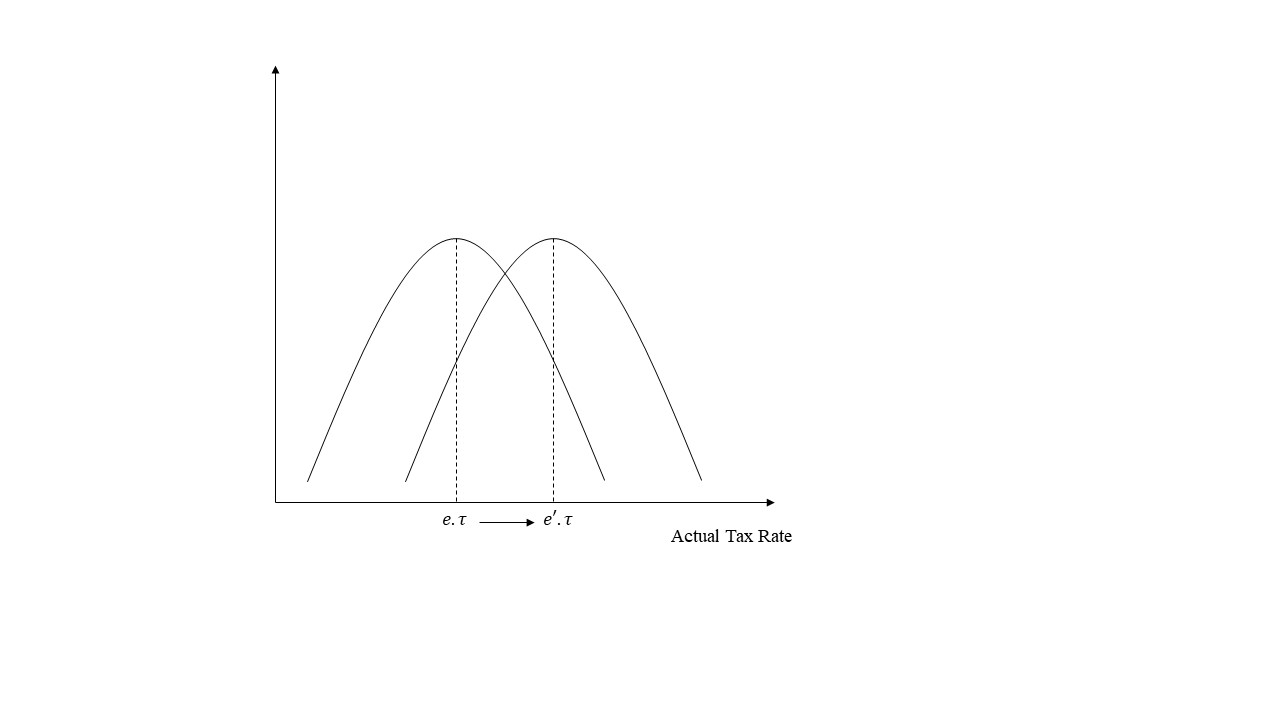
\includegraphics[scale=0.7]{Chapter-5/Figures/laffer.jpg}
%     \caption[Laffer Curve for Tax Collection Effort]{Laffer Curve for Tax Collection Effort
%         \texttt{} }
%     \label{laffer}
% \end{figure}

However, if both central and local governments prioritize welfare-related production expenditures beyond a certain threshold, the situation changes. In this case, increasing general transfers will encourage local governments to allocate more resources to the provision of welfare-related public goods. Consequently, increasing taxes will only exacerbate the crowding-out effect of high tax burdens on total production $F$. Therefore, increasing general transfers will instead prompt local governments to seek ways to alleviate tax burdens.

\subsection{The effect of categorical grants in productive area on tax collection effort}

Since $0<m<1$, whether equation \ref{mone} is positive or not is decided by denominator. Similarly, $1+\frac{\alpha \lambda_i(1-\sigma_i)}{1-\tau_i}$ also acts as a threshold. From the calculation, we have:

\begin{itemize}
    \item When $n_i+\lambda_i<1+\frac{\alpha \lambda_i(1-\sigma_i)}{1-\tau_i}$, $\frac{d \tau_i}{d m_i}>0$
    \item When $n_i+\lambda_i>1+\frac{\alpha \lambda_i(1-\sigma_i)}{1-\tau_i}$,$\frac{d \tau_i}{d m_i}<0$
\end{itemize}

When both national and subnational governments care less about welfare oriented spending, more categorical transfer on productive public goods would stimulate a higher tax collection effort, vice versa.

In the realm of categorical transfers, the effect of increasing the subsidy ratio for productive transfers by the central government on local tax efforts is entirely consistent with the increase in general transfers. This is not surprising, as even without restrictions on the usage domain of general transfers when both local and central governments prioritize productive public goods over welfare-related ones, local governments will still allocate more revenue to productive public goods. This parallels the effect of the central government stipulating a high matching ratio $m$ to encourage local governments to invest more in productive areas.

When both national and subnational governments care about the welfare oriented public goods such that $n+\lambda_i$ surpass the threshold, the greater matching ratio on productive public goods would not stimulate subnational government to invest more on productive spending. On the contrary, the relief on the productive investment would lead to lower revenue gap thus lower the tax collection effort.

\subsection{The effect of categorical grants in welfare area on tax collection effort}
The calculation and the expression of $\frac{\partial e_{i,t}}{\partial n}$ is complicated. I got the expression through Mathematica, the result is shown in figure \ref{enenen}.
% \begin{figure}[H]
%     \centering
%     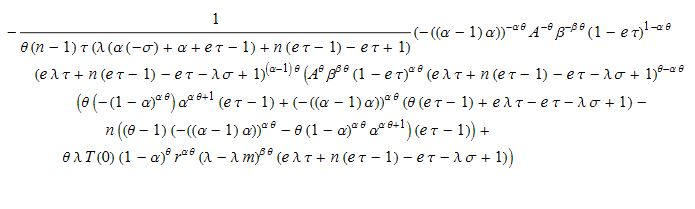
\includegraphics[scale=0.8]{Chapter-5/Figures/calculation effortttt.JPG}
%     \caption[Expression of $\frac{\partial e_{i,t}}{\partial n}$]{Expression of $\frac{\partial e_{i,t}}{\partial n}$
%         \texttt{} }
%     \label{enenen}
% \end{figure}

This expression is very complicated and hard to distinguish whether it's positive or negative, which means the effect of matching ratio of welfare-oriented public spending is ambiguous. We hypothesize that when the national government increases categorical transfers for welfare, it simultaneously incentivizes local governments to further increase the utility derived from welfare expenditures, thereby encouraging higher taxation. However, the role of taxation in economic growth is uncertain. Subnational government may want to decrease the tax collection revenue to boost the economic growth, since the investment in welfare is guaranteed by the subsidy. Therefore, the impact of increased welfare transfers on taxation incentives is uncertain.

For the following of this paper, I'll design an empirical investigation to statistically test my theoretical conjecture.

\section{Regression Model Design and Hypothesis}

This section is to give some general explain of the regression setting, such as the included factors and the regression model. In addition, I give my hypothesis about some of the factors based on the theoretical conjecture I get from previous Ramsey model.

The regression is to distinguish the effect of different kinds of intergovernmental transfer on the tax collection effort. Therefore, the dependent variable of this regression is the tax collection effort, which has been corrected using the Kalman filter algorithm. The specific algorithmic process will be detailed in subsequent sections. The independent variables consist of the ratio of general-purpose transfer payments to specific-purpose transfer payments. Our interest lies in exploring the impact of the growth or reduction of these ratio on tax collection efforts.

Based on our discussion of the theoretical model, there exists a "threshold effect" in the impact of general-purpose and specific-purpose transfer payments on tax collection efforts. The degree of emphasis placed by the federal and state governments on welfare-related public expenditures, represented as $n_i+\lambda_i$ plays a pivotal role in serving as such a threshold. Based on this theoretical inference, a moderating effect model would be particularly helpful in addressing our inquiry. Specifically, it would investigate how the effects of general-purpose and specific-purpose transfer payments on tax collection efforts are moderated by the degree of emphasis placed by the federal and state governments on welfare-related public expenditures.

\section{Variables and Sample}

This subsection is constructed to explain the meaning of the variables and how it's measured. The most important part is to explain the construction of moderating variables and how the dependent variable---tax collection effort is captures.

\subsection{Construction of moderating variables}
The moderating effect in this study exists between two pairs of variables: the variable $Ratio\_gen$, reflecting general-purpose transfer payments, and the variable $w_preference$ representing the degree of emphasis placed by the federal and local governments on welfare expenditures, respectively. Additionally, the moderating effect exists between the variable "transfer payments with purpose constraints" $Ratio\_cons$ and $w_preference$ Therefore, my regression model comprises two regression equations.

\begin{equation}
    TE_{i,t}=a+ \beta_1 Ratio\_gen_{i,t}+\beta_2 w\_preference_{i,t}+\beta_3(Ratio\_gen_{i,t}\cdot w\_preference_{i,t}) +\alpha_i CV_{i,t} \label{reg1}
\end{equation}

\begin{equation}
    TE_{i,t}=a+ \beta_4 Ratio\_cons_{i,t}+\beta_2 w\_preference_{i,t}+\beta_5(Ratio\_cons_{i,t}\cdot w\_preference_{i,t}) +\alpha_i CV_{i,t} \label{reg2}
\end{equation}

where CV means a set of control variables including ratio of different industrial sectors in the whole economy, such as agriculture, manufacturing, finance and insurance, trade and real estate and some factors reflecting economic condition such as gdp per capita, per capita expenditure, median household income and unemployment rate.


The construction of interacting variables is in regression \ref{reg1} and \ref{reg2} needs the representing of the general grants ratio $Ratio\_gen_{i,t}$, matching ratio on productive spending $Ratio\_cons_{i,t}$, and both level of governments' preference on welfare spending $w\_preference_{i,t}$.

From \textit{State Expenditure Annual Report} published by different state governments, I can classify federal and state governments' spending purpose into spending on productive and welfare oriented area. In addition, I can tell the source of the revenue by distinguishing if the grants is offered by federal or state governments. According to former investigation related to the classification of welfare spending and productive spending \parencite{AnpingZhao2012welfareexpenditure,lindbeck1988welfare,wlezien2021trends,stichnoth2013ethnic,schneider2005elite}, I group the spending on education, assistance on needy, cash assistance, medicaid, corrections as welfare spending and spending on transportation, housing and environment as productive expenditure\footnote{The abbreviation for welfare expenditure is marked as "W" in table \ref{expenditure} and productive expenditure is marked as "P". }.As also shown in table \ref{expenditure}, I can calculate whether the grants come from federal or states. Therefore I have the ratio of welfare expenditure of state and national government to represent the preference on welfare spending $w\_preferernce$.

White house Office of Management and Budget supplied publish federal's total outlay every year, in which we can find the proxy of general grants amounts  under "Federal funds" account and grants with constraint amounts under "Trust funds". The general grants amounts is clearly defined, while the ratio of productive grants and welfare grants need to be distinguished manually.

Every state in America is included in my sample and the time span last from 2000 to 2019, unless some specific data is missed.


% \begin{table}[htbp]
%     \centering
%     \caption{State Expenditure Purpose and Revenue Source}
%     \begin{tabular}{|l|c|c|c|c|r|}
%         \toprule
%                                                                                                 & \multicolumn{1}{p{4.355em}|}{General funds} & \multicolumn{1}{p{4.07em}|}{Federal funds} & \multicolumn{1}{p{5em}|}{Other State funds} & \multicolumn{1}{p{4.145em}|}{Bond funds} & \multicolumn{1}{p{6.785em}|}{\textit{\textbf{Expenditure Purposes}}} \\
%         \midrule
%         \multicolumn{1}{|p{9.93em}|}{Elementary \& Secondary Education }                        &                                             &                                            &                                             &                                          & \multicolumn{1}{c|}{\textbf{W}}                                      \\
%         \cmidrule{2-6}    \multicolumn{1}{|p{9.93em}|}{Higher Education }                       &                                             &                                            &                                             &                                          & \multicolumn{1}{c|}{\textbf{W}}                                      \\
%         \cmidrule{2-6}    \multicolumn{1}{|p{9.93em}|}{Temporary Assistance for Needy Families} &                                             &                                            &                                             &                                          & \multicolumn{1}{c|}{\textbf{W}}                                      \\
%         \cmidrule{2-6}    \multicolumn{1}{|p{9.93em}|}{Other Cash Assistance}                   &                                             &                                            &                                             &                                          & \multicolumn{1}{c|}{\textbf{W}}                                      \\
%         \cmidrule{2-6}    \multicolumn{1}{|p{9.93em}|}{Medicaid Total Funds}                    &                                             &                                            &                                             &                                          & \multicolumn{1}{c|}{\textbf{W}}                                      \\
%         \cmidrule{2-6}    \multicolumn{1}{|p{9.93em}|}{Corrections }                            &                                             &                                            &                                             &                                          & \multicolumn{1}{c|}{\textbf{W}}                                      \\
%         \cmidrule{2-6}    \multicolumn{1}{|p{9.93em}|}{Transportation }                         &                                             &                                            &                                             &                                          & \multicolumn{1}{c|}{\textbf{P}}                                      \\
%         \cmidrule{2-6}    \multicolumn{1}{|p{9.93em}|}{Housing Capital }                        &                                             &                                            &                                             &                                          & \multicolumn{1}{c|}{\textbf{P}}                                      \\
%         \cmidrule{2-6}    \multicolumn{1}{|p{9.93em}|}{Enviromental Capital }                   &                                             &                                            &                                             &                                          & \multicolumn{1}{c|}{\textbf{P}}                                      \\
%         \midrule
%         \textit{\textbf{Revenue Source}}                                                        & \textbf{State}                              & \textbf{Federal}                           & \textbf{State}                              & \textbf{---------}                       &                                                                      \\
%         \bottomrule
%     \end{tabular}%
%     \label{expenditure}%
% \end{table}%


The explain of the moderating effects coefficients are different compared to the normal regression. For example, in equation \ref{reg1}, $\beta_1$ is not the effect of general transfer on tax collection effort. To investigate the effect of general transfer ratio on dependent variable, I need to calculate $\frac{\partial TE_{i,t}}{\partial Ratio\_gen_{i,t}}$, thus I have:

$$\frac{\partial TE_{i,t}}{\partial Ratio\_gen_{i,t}}=\beta_1+\beta_3 \cdot w\_preference_{i,t} $$

Therefore, $\beta_1$ is not the effect of general transfer on the tax collection effect, rather, it means the effect of general transfer when $w\_preferernce_{i,t}=0$. As $w\_preferernce_{i,t}$ gets greater, we can tell the effect of general transfer on tax effort by analyzing $\beta_1+\beta_3$. This feature fits our previous theoretical conjecture perfectly since the preference on welfare public spending plays an threshold effect. We can better investigate this threshold effect through the moderating effect regression model. Based on the explain of this moderating effect regression and previous theoretical conjecture, I generated the first hypothesis.
\begin{itemize}
    \item \textbf{Hypothesis 1: Tax effort gets higher as general transfer ratio gets higher when both federal and state governments make light of welfare-oriented public spending. }
\end{itemize}

This hypotheses comes from the theoretical conjecture of the general transfer ratio. In the regression, my expectation is that $\beta_1$ is a significant positive value while $\beta_3$ is a significant negative value. In that way, the effect of general transfer ratio on tax collection effort is negative when $w_preference$ doesn't exceed the threshold. Once the $w_preference$ pass the specific threshold value, the increase of general transfer discourage the tax collection effort.

Similarly, I can have the hypotheses about the effect of productive categorical transfer increase on tax collection effort.

\begin{itemize}
    \item \textbf{Hypothesis 2: Tax effort gets higher as productive categorical transfer ratio gets higher when both federal and state governments make light of welfare-oriented public spending. }
\end{itemize}

The effect of productive categorical transfer follows same logic with the general transfers. Whether the increase of productive categorical transfer stimulates or suppress tax collection effort depends on if federal and state governments' preference on welfare spending surpass a specific threshold. Therefore I'm expecting a significant positive $\beta_4$ and negative $\beta_5$. When $w_preference$ gets greater, the effect of productive categorical transfer became negative.



\subsection{Measure of tax collection effort}

In terms of the dependent variable, tax collection effort, two methods are commonly employed: the average tax ratio method and the potential tax revenue method\parencite*{tait1978two,tanzi1981taxation,tanzi1983quantitative}. The former entails substituting the unobservable variable of tax collection with a proximate and measurable variable. Conversely, the latter method involves comparing the actual tax burden to the predicted tax burden using regression analysis, which is also called as "tax handle" method. According to \textcite{bahl1971regression}, an index of 1 means the tax effort is at the “expected” level, given the structural factors of that country. In other words, the country is using its taxable capacity at a level consistent with the average of the other countries in the sample \parencite{mertens2003measuring}.

However, \textcite{doi:10.1080/13504850500425345} has demonstrated that while the second method, compared to the first, provides relatively more reliable estimates of tax collection effort, both methods are inherently biased. In the same article, \textcite{doi:10.1080/13504850500425345} proposed a solution to this issue by using the Kalman filter to correct tax collection effort and proved its efficiency and unbiasedness in estimating tax collection effort. Therefore, this article also employs this approach to estimate tax collection effort for each state. Specifically, following Kim's methodology, the Kalman filter estimation of tax collection effort involves the following processes.

The state-space model is represented as:
\begin{equation}
    Y_t=\gamma X_t+\alpha A_t+\varepsilon_t \label{statespace1}
\end{equation}

\begin{equation}
    X_{t+1}=\beta X_t+\omega_{t+1}\label{statespace2}
\end{equation}

where $Y_t$ is the tax revenue at time $t$, $X_t$ is tax effort and $A_t$ is a vector of other factors affecting tax revenue except for tax effort. The error terms $\varepsilon_t$ and $\omega_{t}$ are both serially uncorrelated with a mean of zero and a covariance matrix $h_t$ and $q_t$ respectively. Therefore we have:

\begin{equation}
    (\begin{array}{l}\varepsilon_t \\ \omega_t\end{array}) \sim N\left(\left(\begin{array}{l}0 \\ 0\end{array}\right) ,\left(\begin{array}{ll}h_t & 0 \\ 0 & q_t\end{array}\right)\right) \label{ssvar}
\end{equation}

$X_t$ has a known mean $a_0 $and a variance $b_0$. Therefore, if the variances of the error terms and the initial values of revenue effort and its variance are known, tax revenue effort can be derived with the following Kalman filter equations \parencite{doi:10.1080/13504850500425345}:

\begin{equation}
    \hat{X}_{t+1,t}=\tau \hat{X}_{t,t}\label{k1}
\end{equation}

\begin{equation}
    P_{t+1,t}=\tau^2 P_{t,t}+q^2
\end{equation}

\begin{equation}
    B_{t+1,t}=\alpha^2 P_{t+1,t}+h^2
\end{equation}

\begin{equation}
    \hat{\epsilon}_{t+1,t}=Y_{t+1}-\alpha \hat{X}_{t+1,t}-\beta A_{t+1}
\end{equation}

\begin{equation}
    K_{t+1}=P_{t+1,t}\alpha B^{-1}_{t+1,t}
\end{equation}

\begin{equation}
    \hat{X}_{t+1,t+1}=\hat{X}_{t+1,t}+K_{t+1}\hat{\epsilon}_{t+1,t}
\end{equation}

\begin{equation}
    P_{t+1,t+1}=(1-K_{t+1}\alpha)P_{t+1,t}\label{k7}
\end{equation}

From equation \ref{k1} to equation \ref{k7}, I can get a kalman filter processed series data \{$X_{t,t}$\} of each state i. Now I need to specify the state-space model formed up by measurement equation, which is equation \ref{statespace1} and transition equation, which is equation \ref{statespace2}.

Equation \ref{statespace1} is the commonly used "tax handle" regression. I focus on the tax collection effort of states governments, thus the commonly used tax handle should includes the factors that reflect the economic structure. Based on the North American Industry Classification System (NAICS), I categorized all industries into 11 major groups: Agriculture; Mining; Manufacturing; Wholesale trade and retail trade; Transportation and warehousing; Information; Finance and insurance; Real estate, rental, and leasing; Health care and social assistance; Professional, scientific, educational, and technical services. I'll calculate the ratio of each industries compared to state GDP and make it as tax handles. Besides, the commonly used control variables to predict the tax revenue includes GDP per capita, median household income and unemployment rate. Therefore the variables included in $A_t$ can be listed as table \ref{handlevariables}.
% Table generated by Excel2LaTeX from sheet 'xtregionolsss0212'
% \begin{table}[htbp]
%     \centering
%     \caption{Tax handle variables to predict the tax revenue}
%     \begin{tabular}{cl}
%         \toprule
%         Abbreviation & Meaning                                                       \\
%         \midrule
%         agrr         & Ratio of agriculture to gdp                                   \\
%         minr         & Ratio of mining to gdp                                        \\
%         manr         & Ratio of manufacturing to gdp                                 \\
%         tandwr       & Ratio of transportation and warehouse to gdp                  \\
%         infr         & Ratio of information to gdp                                   \\
%         fandir       & Ratio of finance and insurance to gdp                         \\
%         rer          & Ratio of real estate to gdp                                   \\
%         hsr          & Ratio of health care and social assistance to gdp             \\
%         piepcm       & per capital income spend on expenditure                       \\
%         trader       & Ratio of trade to gdp                                         \\
%         pster        & Professional, scientific, educational, and technical services \\
%         mehim        & Median household income                                       \\
%         unemployrate & unemployment rate                                             \\
%         gdp          & GDP per capita                                                \\
%         \bottomrule
%     \end{tabular}%
%     \label{handlevariables}%
% \end{table}%

Given the diverse economic structures across different regions in the United States, industries serving as tax bases vary. Recognizing the variation in tax bases created by different economic structures in various regions, I segmented the data by region to conduct fixed-effects regressions based on the U.S. Department of Commerce Bureau of Economic Analysis' classification of regions , aiming to maximize the adjusted R-squared and enhance predictive accuracy. Those 8 segments are: Far West, Great Lakes, Mideast, New England,	Plains,	Rocky Mountain,	Southeast, Southwest.

The DF test result, shown in table \ref{DFtest} for each variable within each region shows that some time series data are not stationary, which contradicts with the assumption of equation \ref{ssvar}. Therefore before the tax handle regression, I conduct the 1 st order difference for the variables that do not pass the DF test and make sure all variables of states $i$ are stationary before conducting the tax handle regression \footnote{Table \ref{DFtest} only shows part of the DF test results. For full results, please visit the appendix part}.

% Table generated by Excel2LaTeX from sheet 'processedDFTEST0212'
% \begin{table}
%     \centering
%     \caption{DF test results for variables in state of America}
%     \resizebox{17cm}{11cm}{
%         \begin{tabular}{llrrrrrrrrrrrrrrr}
%             \toprule
%             geoname     & level\_1      & \multicolumn{1}{l}{taxrevenueratio} & \multicolumn{1}{l}{agrr} & \multicolumn{1}{l}{minr} & \multicolumn{1}{l}{manr} & \multicolumn{1}{l}{tandwr} & \multicolumn{1}{l}{infr} & \multicolumn{1}{l}{fandir} & \multicolumn{1}{l}{rer} & \multicolumn{1}{l}{hsr} & \multicolumn{1}{l}{piepcm} & \multicolumn{1}{l}{trader} & \multicolumn{1}{l}{pster} & \multicolumn{1}{l}{mehim} & \multicolumn{1}{l}{unemployrate} & \multicolumn{1}{l}{gdppercapita} \\
%             \midrule
%             Alabama     & ADF Statistic & -2.9584957                          & -4.0738483               & -2.1262916               & -3.7780187               & -2.3795241                 & -4.5285992               & -2.8465617                 & -3.3691314              & -6.6545878              & -2.3099791                 & -0.354905                  & -4.7383288                & -5.2118955                & -2.5388273                       & -2.4977533                       \\
%             Alabama     & P-value       & 0.1440567                           & 0.0068865                & 0.531346                 & 0.0177068                & 0.3905597                  & 0.0013549                & 0.1803687                  & 0.0556509               & 8.41E-08                & 0.4284382                  & 0.9881567                  & 0.0005996                 & 8.32E-05                  & 0.3088295                        & 0.3290865                        \\
%             Alaska      & ADF Statistic & -2.0826184                          & -3.1155341               & -3.7940843               & -3.3981553               & -6.4811537                 & -2.6940316               & -4.9448154                 & -4.5470878              & -5.6889734              & -3.1354863                 & -7.3714471                 & -3.0392903                & -1.7603157                & -2.7177455                       & -2.7181459                       \\
%             Alaska      & P-value       & 0.5558153                           & 0.1025832                & 0.0168625                & 0.0516349                & 2.03E-07                   & 0.238569                 & 0.000259                   & 0.0012629               & 9.64E-06                & 0.0980398                  & 2.01E-09                   & 0.1214254                 & 0.7235718                 & 0.2287886                        & 0.2286257                        \\
%             Arizona     & ADF Statistic & -3.8693215                          & -4.6322823               & -1.7101206               & -0.3743152               & -7.5316714                 & -4.4778336               & -4.1707467                 & -5.3301527              & -2.5375428              & -2.0054682                 & -2.3710659                 & -3.7761038                & -6.1423639                & -1.9470851                       & -2.5295149                       \\
%             Arizona     & P-value       & 0.0133634                           & 0.0009099                & 0.7464038                & 0.9876256                & 8.62E-10                   & 0.0016406                & 0.0049542                  & 4.95E-05                & 0.3094533               & 0.5984518                  & 0.3951099                  & 0.0178099                 & 1.10E-06                  & 0.6299357                        & 0.3133664                        \\
%             Arkansas    & ADF Statistic & -3.8144652                          & -3.2574705               & -3.3138418               & -3.2526213               & -2.6120583                 & -3.0102396               & -5.2714893                 & -1.9617547              & -3.8665392              & -2.8672628                 & 0.7610834                  & -3.8232961                & -7.2296709                & -1.8315081                       & -2.9306735                       \\
%             Arkansas    & P-value       & 0.0158426                           & 0.0735461                & 0.0640084                & 0.0744169                & 0.2743734                  & 0.1292407                & 6.41E-05                   & 0.6221029               & 0.0134803               & 0.1733367                  & 1                          & 0.0154179                 & 4.25E-09                  & 0.6893708                        & 0.1525052                        \\
%             California  & ADF Statistic & -3.3335918                          & 0.7247841                & -5.2060476               & -2.2999803               & -3.9951928                 & -1.4944674               & -3.301189                  & -5.0087446              & -5.1396849              & -2.3659968                 & -2.8818869                 & -3.6344666                & -2.2391546                & -2.2533527                       & -2.8013711                       \\
%             California  & P-value       & 0.0609133                           & 1                        & 8.53E-05                 & 0.4339608                & 0.008933                   & 0.8310186                & 0.0660573                  & 0.0001983               & 0.0001137               & 0.3978451                  & 0.1684937                  & 0.027052                  & 0.4678524                 & 0.4599033                        & 0.1964413                        \\
%             Colorado    & ADF Statistic & -7.6191717                          & -3.3285227               & -0.8284793               & -2.0928674               & -2.7511687                 & -2.1354386               & -4.6806141                 & -2.6886979              & -4.714105               & -2.3839804                 & -1.2484704                 & -3.8171345                & -4.353958                 & -2.0836961                       & -2.559226                        \\
%             Colorado    & P-value       & 5.42E-10                            & 0.0616959                & 0.9631981                & 0.5500885                & 0.2154567                  & 0.5262035                & 0.0007533                  & 0.2408052               & 0.0006601               & 0.3881694                  & 0.9000907                  & 0.0157131                 & 0.0025905                 & 0.5552137                        & 0.2990106                        \\
%             Connecticut & ADF Statistic & 0.105427                            & -5.614409                & -2.6514881               & -3.7322998               & -3.3657117                 & -2.1895655               & -3.9815021                 & -2.9085756              & -3.7505465              & -2.7743348                 & -2.5193086                 & -3.2045364                & -2.5030802                & -3.7037153                       & -4.7590079                       \\
%             Connecticut & P-value       & 0.9951566                           & 1.36E-05                 & 0.2567715                & 0.0203164                & 0.0561405                  & 0.495725                 & 0.0093407                  & 0.1594584               & 0.0192371               & 0.2065306                  & 0.3183769                  & 0.0835016                 & 0.326424                  & 0.0221138                        & 0.0005522                        \\
%             Delaware    & ADF Statistic & -3.1393466                          & -3.3145667               & -4.9336125               & -3.2188079               & -0.7223429                 & -2.303585                & -0.6156446                 & -3.3056062              & -4.247519               & -2.7340805                 & -3.7018074                 & -5.8610316                & -4.7405574                & -3.2199067                       & -10.574259                       \\
%             Delaware    & P-value       & 0.0971789                           & 0.0638926                & 0.0002713                & 0.0807187                & 0.9716374                  & 0.431968                 & 0.9781385                  & 0.0653361               & 0.0037908               & 0.2222062                  & 0.0222385                  & 4.28E-06                  & 0.0005943                 & 0.0805075                        & 1.51E-16                         \\
%             Florida     & ADF Statistic & -4.8669747                          & -2.7072056               & -4.2669358               & -5.5067657               & -2.6650288                 & -0.4769127               & -1.9741621                 & -3.3385817              & -3.0333683              & -3.0453498                 & -2.4700988                 & -5.2922004                & -2.136408                 & -2.542309                        & -2.5571086                       \\
%             Florida     & P-value       & 0.0003569                           & 0.2331029                & 0.0035394                & 2.23E-05                 & 0.2508878                  & 0.9843121                & 0.6154352                  & 0.0601509               & 0.1229896               & 0.1198402                  & 0.3430694                  & 5.85E-05                  & 0.5256582                 & 0.307142                         & 0.3000221                        \\
%             Georgia     & ADF Statistic & -1.3862558                          & -3.9642423               & -1.5576629               & -3.974274                & -1.4218962                 & -1.0532807               & -2.1118196                 & -3.6462642              & -4.011087               & -2.0314994                 & -3.7304951                 & -2.7878658                & -2.8849757                & -2.4816295                       & -0.3230385                       \\
%             Georgia     & P-value       & 0.8649024                           & 0.0098784                & 0.8085722                & 0.0095626                & 0.8543696                  & 0.9365038                & 0.5394719                  & 0.0261488               & 0.0084799               & 0.5841755                  & 0.020426                   & 0.2014369                 & 0.1674839                 & 0.3372069                        & 0.9889707                        \\
%             Hawaii      & ADF Statistic & -3.2823748                          & -3.4492431               & -2.0175917               & -0.9805192               & -4.2261142                 & -3.5835385               & -4.2564581                 & 0.1945429               & -2.9148399              & -1.8186507                 & -3.3759258                 & -1.5834406                & -0.9607372                & -3.2727731                       & -2.0802754                       \\
%             Hawaii      & P-value       & 0.0692012                           & 0.045148                 & 0.591819                 & 0.9466804                & 0.0040869                  & 0.0312658                & 0.0036731                  & 0.9957462               & 0.1574654               & 0.6956964                  & 0.0546885                  & 0.79885                   & 0.9491729                 & 0.0708514                        & 0.5571229                        \\
%             Idaho       & ADF Statistic & -4.272711                           & -3.4487125               & -1.8967678               & -3.0275766               & -3.109667                  & -2.7050241               & 0.1819603                  & -2.7692856              & -4.7744075              & -2.9283954                 & 0.1210051                  & -3.6201161                & -11.799223                & -2.9882011                       & -3.5448589                       \\
%             Idaho       & P-value       & 0.0034676                           & 0.0452117                & 0.6563424                & 0.1245337                & 0.1039492                  & 0.2340024                & 0.9956721                  & 0.2084541               & 0.0005192               & 0.153212                   & 0.995271                   & 0.0281867                 & 8.23E-19                  & 0.1354096                        & 0.0348303                        \\
%             Illinois    & ADF Statistic & 2.2055768                           & -4.5868314               & -2.9059329               & -2.9685475               & -4.9050819                 & -4.0010139               & -3.1577302                 & -4.0337167              & -3.3368733              & -2.8416788                 & -2.1622079                 & -4.5311699                & -4.8661301                & -2.6609907                       & -3.1650605                       \\
%             Illinois    & P-value       & 1                                   & 0.0010847                & 0.1603045                & 0.1410877                & 0.0003053                  & 0.0087646                & 0.0931582                  & 0.0078705               & 0.0604111               & 0.1820576                  & 0.5111346                  & 0.0013417                 & 0.0003581                 & 0.2526337                        & 0.0915913                        \\
%             Indiana     & ADF Statistic & -5.1574461                          & -5.7155784               & -2.1507255               & -6.4777512               & -3.06508                   & -5.2218945               & -7.0097004                 & -6.1401189              & -7.8039373              & -2.436235                  & -2.3102721                 & -3.0872072                & -0.7023714                & -2.9533594                       & -3.6019904                       \\
%             Indiana     & P-value       & 0.0001053                           & 8.51E-06                 & 0.5176008                & 2.06E-07                 & 0.1147847                  & 7.96E-05                 & 1.34E-08                   & 1.11E-06                & 2.03E-10                & 0.3605396                  & 0.4282766                  & 0.1093063                 & 0.9729916                 & 0.1455909                        & 0.0296783                        \\
%             Iowa        & ADF Statistic & -6.0901826                          & -4.3927572               & -2.4832443               & -7.0679353               & -2.6322937                 & -1.9978792               & -5.5354435                 & -3.1579108              & -4.6701772              & -3.2590251                 & -3.2725052                 & -2.7406905                & -6.0708915                & -2.9988559                       & -4.9323914                       \\
%             Iowa        & P-value       & 1.42E-06                            & 0.0022487                & 0.3363895                & 9.91E-09                 & 0.2652539                  & 0.6025886                & 1.96E-05                   & 0.0931194               & 0.0007848               & 0.0732687                  & 0.0708978                  & 0.2195788                 & 1.56E-06                  & 0.1324011                        & 0.0002727                        \\
%             Kansas      & ADF Statistic & -2.5665144                          & -3.1387984               & -1.2040844               & 0.61863                  & -2.9471436                 & -4.2537381               & -2.7062164                 & -2.4390351              & -0.5887284              & -3.0432453                 & -2.7899665                 & -4.5161056                & -3.8964404                & -2.7820881                       & -4.1499461                       \\
%             Kansas      & P-value       & 0.2955427                           & 0.0973008                & 0.9096626                & 0.9970018                & 0.1474629                  & 0.0037085                & 0.2335105                  & 0.3590813               & 0.9795168               & 0.120389                   & 0.2006541                  & 0.0014205                 & 0.0122702                 & 0.2036011                        & 0.0053214                        \\
%             Kentucky    & ADF Statistic & -3.7910525                          & -2.556417                & -4.9316617               & -2.4623514               & -3.140775                  & -2.6790055               & -2.6041511                 & -3.3248058              & -0.7279646              & -2.8402648                 & -2.0194022                 & -0.6672932                & -4.0015556                & -2.519608                        & -4.1190233                       \\
%             Kentucky    & P-value       & 0.0170191                           & 0.3003528                & 0.0002735                & 0.3470336                & 0.0968618                  & 0.2449027                & 0.2779856                  & 0.0622749               & 0.9712438               & 0.1825489                  & 0.590826                   & 0.9752111                 & 0.008749                  & 0.3182293                        & 0.0059134                        \\
%             Louisiana   & ADF Statistic & -3.4668779                          & -7.3993455               & -5.0297387               & -3.123526                & -2.0422269                 & 0.5809776                & -2.7602631                 & -3.158981               & -4.0690225              & -2.6377381                 & -2.5084001                 & -1.8975846                & -3.0377071                & -1.4466776                       & -3.5362443                       \\
%             Louisiana   & P-value       & 0.0430729                           & 1.74E-09                 & 0.0001816                & 0.1007445                & 0.5782566                  & 0.9969685                & 0.2119217                  & 0.0928894               & 0.0069986               & 0.2628312                  & 0.3237753                  & 0.6559199                 & 0.1218422                 & 0.8466851                        & 0.0356696                        \\
%             \bottomrule
%         \end{tabular}%
%         \label{DFtest}}%
% \end{table}%



Given that the primary objective of this regression equation is prediction, multicollinearity is not a significant concern. The tax handle regression results can be listed as table \ref{taxhandleregressionresult}. In this table, we can tell clearly that the significant industries, which is tax handles that determinant the tax revenue of states, are different. For example, the manufacturing industry is important for states in Plains area, while it's not significant for other areas such as states in far west, great lakes, mideast and new england. This also reflects the significance to predict the revenue and conduct the tax handle regression by region.

The tax handle regression in different regions are listed in Table \ref{taxhandleregressionresult}. After removing the insignificant factors, I get the predicted tax revenue ratio based on the significant tax handles. For example, for states in far west area, the predict formula is listed as:

\begin{equation}
    Tax\_revenue\_predict= tandw* 1.674 + fandi * 1.133 -3.223* hs  + trade * 0.818 + gdppercapita * 0.029 \label{taxhandlefarwest}
\end{equation}



% \begin{table}
%     \centering
%     \caption{Tax handle regression results for regions in America}
%     \resizebox{\textwidth}{8cm}{
%         \begin{tabular}{ccccccccc}
%             \toprule
%                                         & Far West  & Great Lakes & Mideast    & New England & Plains     & Rocky Mountain & Southeast  & Southwest   \\
%             \midrule
%             agrr                        & 0.314     & 0.391       & 0.478      & 1.169       & 0.038      & -0.115         & 0.0381     & 0.69        \\
%                                         & -0.27     & -1.06       & -0.74      & -1.55       & -1.18      & (-0.44)        & -0.29      & -1.53       \\
%             minr                        & 0.185     & 0.031       & 0.653      & -0.248      & 0.156      & -0.0348        & 0.0343     & 0.0859      \\
%                                         & -1.87     & -0.08       & -1.91      & (-0.28)     & -0.87      & (-1.15)        & -0.48      & -1.24       \\
%             manr                        & -0.0354   & 0.0383      & -0.0819    & 0.0375      & -0.130**   & 0.0179         & 0.0746     & -0.0132     \\
%                                         & (-0.30)   & -0.77       & (-0.97)    & -0.74       & (-3.03)    & -0.16          & -1.04      & (-0.31)     \\
%             tandwr                      & 1.674***  & 1.493***    & 1.205***   & -1.131*     & -0.138     & 0.12           & 1.092***   & 0.17        \\
%                                         & -22.19    & -27.17      & -4.2       & (-2.29)     & (-0.89)    & -0.39          & -22.7      & -0.89       \\
%             infr                        & -0.16     & -0.28       & -0.0533    & -0.0324     & -0.0277    & 0.061          & -0.0518    & -0.362*     \\
%                                         & (-0.62)   & (-0.79)     & (-0.65)    & (-0.24)     & (-0.38)    & -0.24          & (-0.32)    & (-2.41)     \\
%             fandir                      & 1.133*    & -0.109      & -0.0168    & 0.0688      & 0.0799*    & -0.268         & -0.541***  & 0.0148      \\
%                                         & -2.76     & (-0.72)     & (-0.37)    & -1.65       & -2.78      & (-1.00)        & (-23.22)   & -0.08       \\
%             rer                         & -0.069    & 0.00559     & -0.120**   & 0.161*      & 0.189***   & -0.0876        & -0.0218    & 0.158***    \\
%                                         & (-0.43)   & -0.84       & (-2.94)    & -2.26       & -4.71      & (-1.24)        & (-0.57)    & -5.85       \\
%             hsr                         & -3.223**  & 0.262       & -0.0815    & 0.317**     & -0.0291    & 1.138*         & 0.756***   & -1.326*     \\
%                                         & (-3.17)   & -0.82       & (-1.19)    & -3.23       & (-0.09)    & -2.23          & -28.81     & (-2.19)     \\
%             piepcm                      & 0.017     & 0.022       & 0.00506*   & 0.00597     & 0.00863    & -0.00616       & 0.00248*   & 0.0329      \\
%                                         & -0.3      & -0.97       & -2.66      & -0.71       & -0.4       & (-1.46)        & -2.24      & -1.17       \\
%             trader                      & 0.818*    & 0.0534      & -0.155**   & -0.105      & 0.0846     & -0.203*        & -0.0765    & -0.209***   \\
%                                         & -2.63     & -0.29       & (-3.57)    & (-0.88)     & -0.46      & (-2.14)        & (-2.06)    & (-7.11)     \\
%             pster                       & -0.45     & 0.0163      & 0.0194     & 0.189       & 0.507      & -0.137         & 0.788***   & -0.146      \\
%                                         & (-1.02)   & -0.89       & -0.21      & -1.86       & -1.88      & (-0.43)        & -35.78     & (-0.59)     \\
%             mehim                       & -0.00209  & 0.000118    & -0.00259*  & 0.00166     & 0.00102    & 0.00367*       & -0.00033   & -0.00409*** \\
%                                         & (-0.90)   & -0.11       & (-2.28)    & -1.61       & -0.79      & -2.44          & (-2.03)    & (-6.63)     \\
%             unemployrate                & 0.00127   & 0.00147     & 0.00128*   & 0.000011    & 0.00227    & 0.00185        & 0.000567** & 0.00187*    \\
%                                         & -1.25     & -1.56       & -2.75      & -0.01       & -1.65      & -1.92          & -3.52      & -2.66       \\
%             gdppercapita                & 0.0295*** & -0.00041    & 0.00397*** & 0.000235    & 0.00632*** & 0.00113        & 0.000338   & -0.0353**   \\
%                                         & -5.38     & (-0.89)     & -4.2       & -0.32       & -7.52      & -0.22          & -1.25      & (-3.52)     \\
%             Constant                    & -0.00177  & -0.00194    & 0.0201*    & -0.0149*    & -0.00177   & 0.0147         & -1.5E-05   & 0.0247***   \\
%                                         & (-0.33)   & (-0.80)     & -2.72      & (-2.76)     & (-0.86)    & -0.64          & (-0.02)    & -5.27       \\
%             \midrule
%             Observations                & 98        & 93          & 87         & 86          & 117        & 79             & 210        & 68          \\
%             Adjusted R-sq               & 0.882     & 0.982       & 0.988      & 0.979       & 0.963      & 0.893          & 0.958      & 0.98        \\
%             \midrule
%             t statistics in parentheses &           &             &            &             &            &                &            &             \\
%             *p<0.05,**p<0.01,***p<0.001 &           &             &            &             &            &                &            &             \\
%             \bottomrule
%         \end{tabular}}%
%     \label{taxhandleregressionresult}%
% \end{table}%

After the tax handle regression, I get the predicted tax revenue ratio for different state. Then I can get the tax collection effort by calculating the predicted value with actual value $\frac{Tax\_revenue\_predict}{Tax\_revenue\_actual}$. Part of the descriptive results is shown in table \ref{taxeffortsum}. Therefore, I have the measurement equation ready among the space-state equations since I have $X_t$ in equation \ref{statespace1} known parameters. In addition, the B-W heteroskedasticity test confirms that regression of equation \ref{statespace1} follows the constant residuals, shown in table \ref{bwtest}

% \begin{table}[htbp]
%     \centering
%     \caption{B-W heteroskedasticity test result for measurement equation regression}
%     \begin{tabular}{llllll}
%         \toprule
%         \multicolumn{6}{c}{Breusch-Pagan / Cook-Weisberg test for heteroskedasticity } \\
%         \midrule
%         \multicolumn{6}{l}{         Ho: Constant variance}                             \\
%         \multicolumn{6}{l}{         Variables: residuals}                              \\
%         \multicolumn{6}{c}{}                                                           \\
%         \multicolumn{6}{l}{         chi2(1)      =     0.88}                           \\
%         \multicolumn{6}{l}{         Prob > chi2  =   0.3491}                           \\
%         \bottomrule
%     \end{tabular}%
%     \label{bwtest}%
% \end{table}%


For transition equations, I assume the transition process follows an AR(1) process and the coefficient of the autocorrelation is 1 since table \ref{taxeffortsum} shows most of the tax effort index lies in [0.7, 1.2] and the standard error is small\footnote{This assumption is not necessarily to be too precise.}.

So far I got the space-state equation prepared and the initial parameters for kalman filter process is known including $\gamma$, $\alpha$, $\alpha$, $X_{0,0}$, $P_{0,0}$. Therefore, through equation \ref{k1} to equation \ref{k7}, I have a new kalman algorithm adjusted series of tax collection effort $\{X_{t,t}\}$.


% \begin{table}[htbp]
%     \centering
%     \caption{Summary of the tax effort level in states(part)}
%     \begin{tabular}{cccccc}
%         \toprule
%                     &     & \multicolumn{4}{c}{Tax collection effort}                               \\
%         \midrule
%         State       & Obs & Mean                                      & Std.    & Min     & Max     \\
%         \midrule
%         Alabama     & 17  & 0.99108                                   & 0.10704 & 0.77345 & 1.12369 \\
%         Alaska      & 18  & 1.15363                                   & 0.63936 & -0.0749 & 2.9033  \\
%         Arizona     & 15  & 0.9645                                    & 0.10226 & 0.80104 & 1.19916 \\
%         Arkansas    & 15  & 0.97468                                   & 0.12192 & 0.85674 & 1.20869 \\
%         California  & 19  & 1.05056                                   & 0.16872 & 0.53894 & 1.23222 \\
%         Colorado    & 19  & 1.01097                                   & 0.10623 & 0.8695  & 1.26189 \\
%         Connecticut & 19  & 0.73208                                   & 0.08448 & 0.6359  & 0.90594 \\
%         Delaware    & 14  & 1.08929                                   & 0.09726 & 0.90916 & 1.2335  \\
%         Florida     & 19  & 1.09674                                   & 0.16283 & 0.87646 & 1.49477 \\
%         Georgia     & 19  & 0.99922                                   & 0.1371  & 0.74665 & 1.34715 \\
%         Hawaii      & 14  & 0.97187                                   & 0.15959 & 0.69107 & 1.18888 \\
%         Idaho       & 19  & 0.91308                                   & 0.11257 & 0.73638 & 1.18433 \\
%         Illinois    & 19  & 1.00037                                   & 0.1077  & 0.82428 & 1.26365 \\
%         Indiana     & 17  & 1.00917                                   & 0.07028 & 0.85208 & 1.13589 \\
%         Iowa        & 17  & 8.06824                                   & 1.30505 & 5.15989 & 9.82793 \\
%         Kansas      & 19  & 1.23506                                   & 0.18167 & 0.9192  & 1.70648 \\
%         Kentucky    & 19  & 0.9929                                    & 0.08475 & 0.87784 & 1.25705 \\
%         \bottomrule
%     \end{tabular}%
%     \label{taxeffortsum}%
% \end{table}%

After the estimation of tax collection effort, I can run regression \ref{reg1} and regression \ref{reg2}. The results can be listed as Table \ref{reg_igt_eff}

\section{Regression Results and Analysis}

The regression result is shown in table \ref{reg_igt_eff}. Both OLS regression and fixed regression, with state and time fixed, are adopted with different variables included. To control the heteroskedasticity problem, I included robust standard error in both regressions. The adjusted R-square and the significance of all models are acceptable, but I adopt the coefficients of fixed effect model as reference, in which state and time variable fixed.

The first hypotheses about the general transfer ratio is supported. From model 4, the coefficient of $generalratio$ is 17.64 and it's significant on 5\% confident level. The coefficient of the interaction variable $int_gen_pref$ is -23.64 and it's also statistically significant. This coefficients combination strongly supported our hypotheses about the effect of general grants on tax collection effort: when federal and state government care less about the welfare-oriented public spending, more general transfer lead to higher tax collection effort. For example, when both levels of governments do not care about welfare at all, which means $n+\lambda=0$, $\frac{\partial\ TE}{\partial generalratio}=\beta_1=17.64$. Once federal or state government attach importance to the welfare product, thus federal increase the matching ratio of welfare spending $n$ and state government get more utility for welfare spending, which makes $n+\lambda_i$ pass the threshold, the marginal effect of general transfer ratio on tax collection effort became negative. For example, when $n+\lambda=1$, $\frac{\partial TE}{\partial generalratio}=\beta_1+\beta_3=-6$.

The second hypothesis is not supported unfortunately. On the contrary, the coefficient of constraint ratio $\beta_4$ in model 3 equals to -14.38 and the coefficient of the interaction term $int_cons_pref$ equals to 19.25. This means that, though we do observe an threshold effect, the effect is not act similarly with general transfer, just the opposite, the marginal effect on the matching ratio on productive spending $m$ is positive when both levels of governments neglect the welfare spending, and such marginal effect turns to negative when $n+\lambda$ exceeds the threshold.

The moderating effect of the two regression models are represented in figure \ref{int_gen_W} and \ref{int_cons_W}.

% \begin{figure}[H]
%     \centering
%     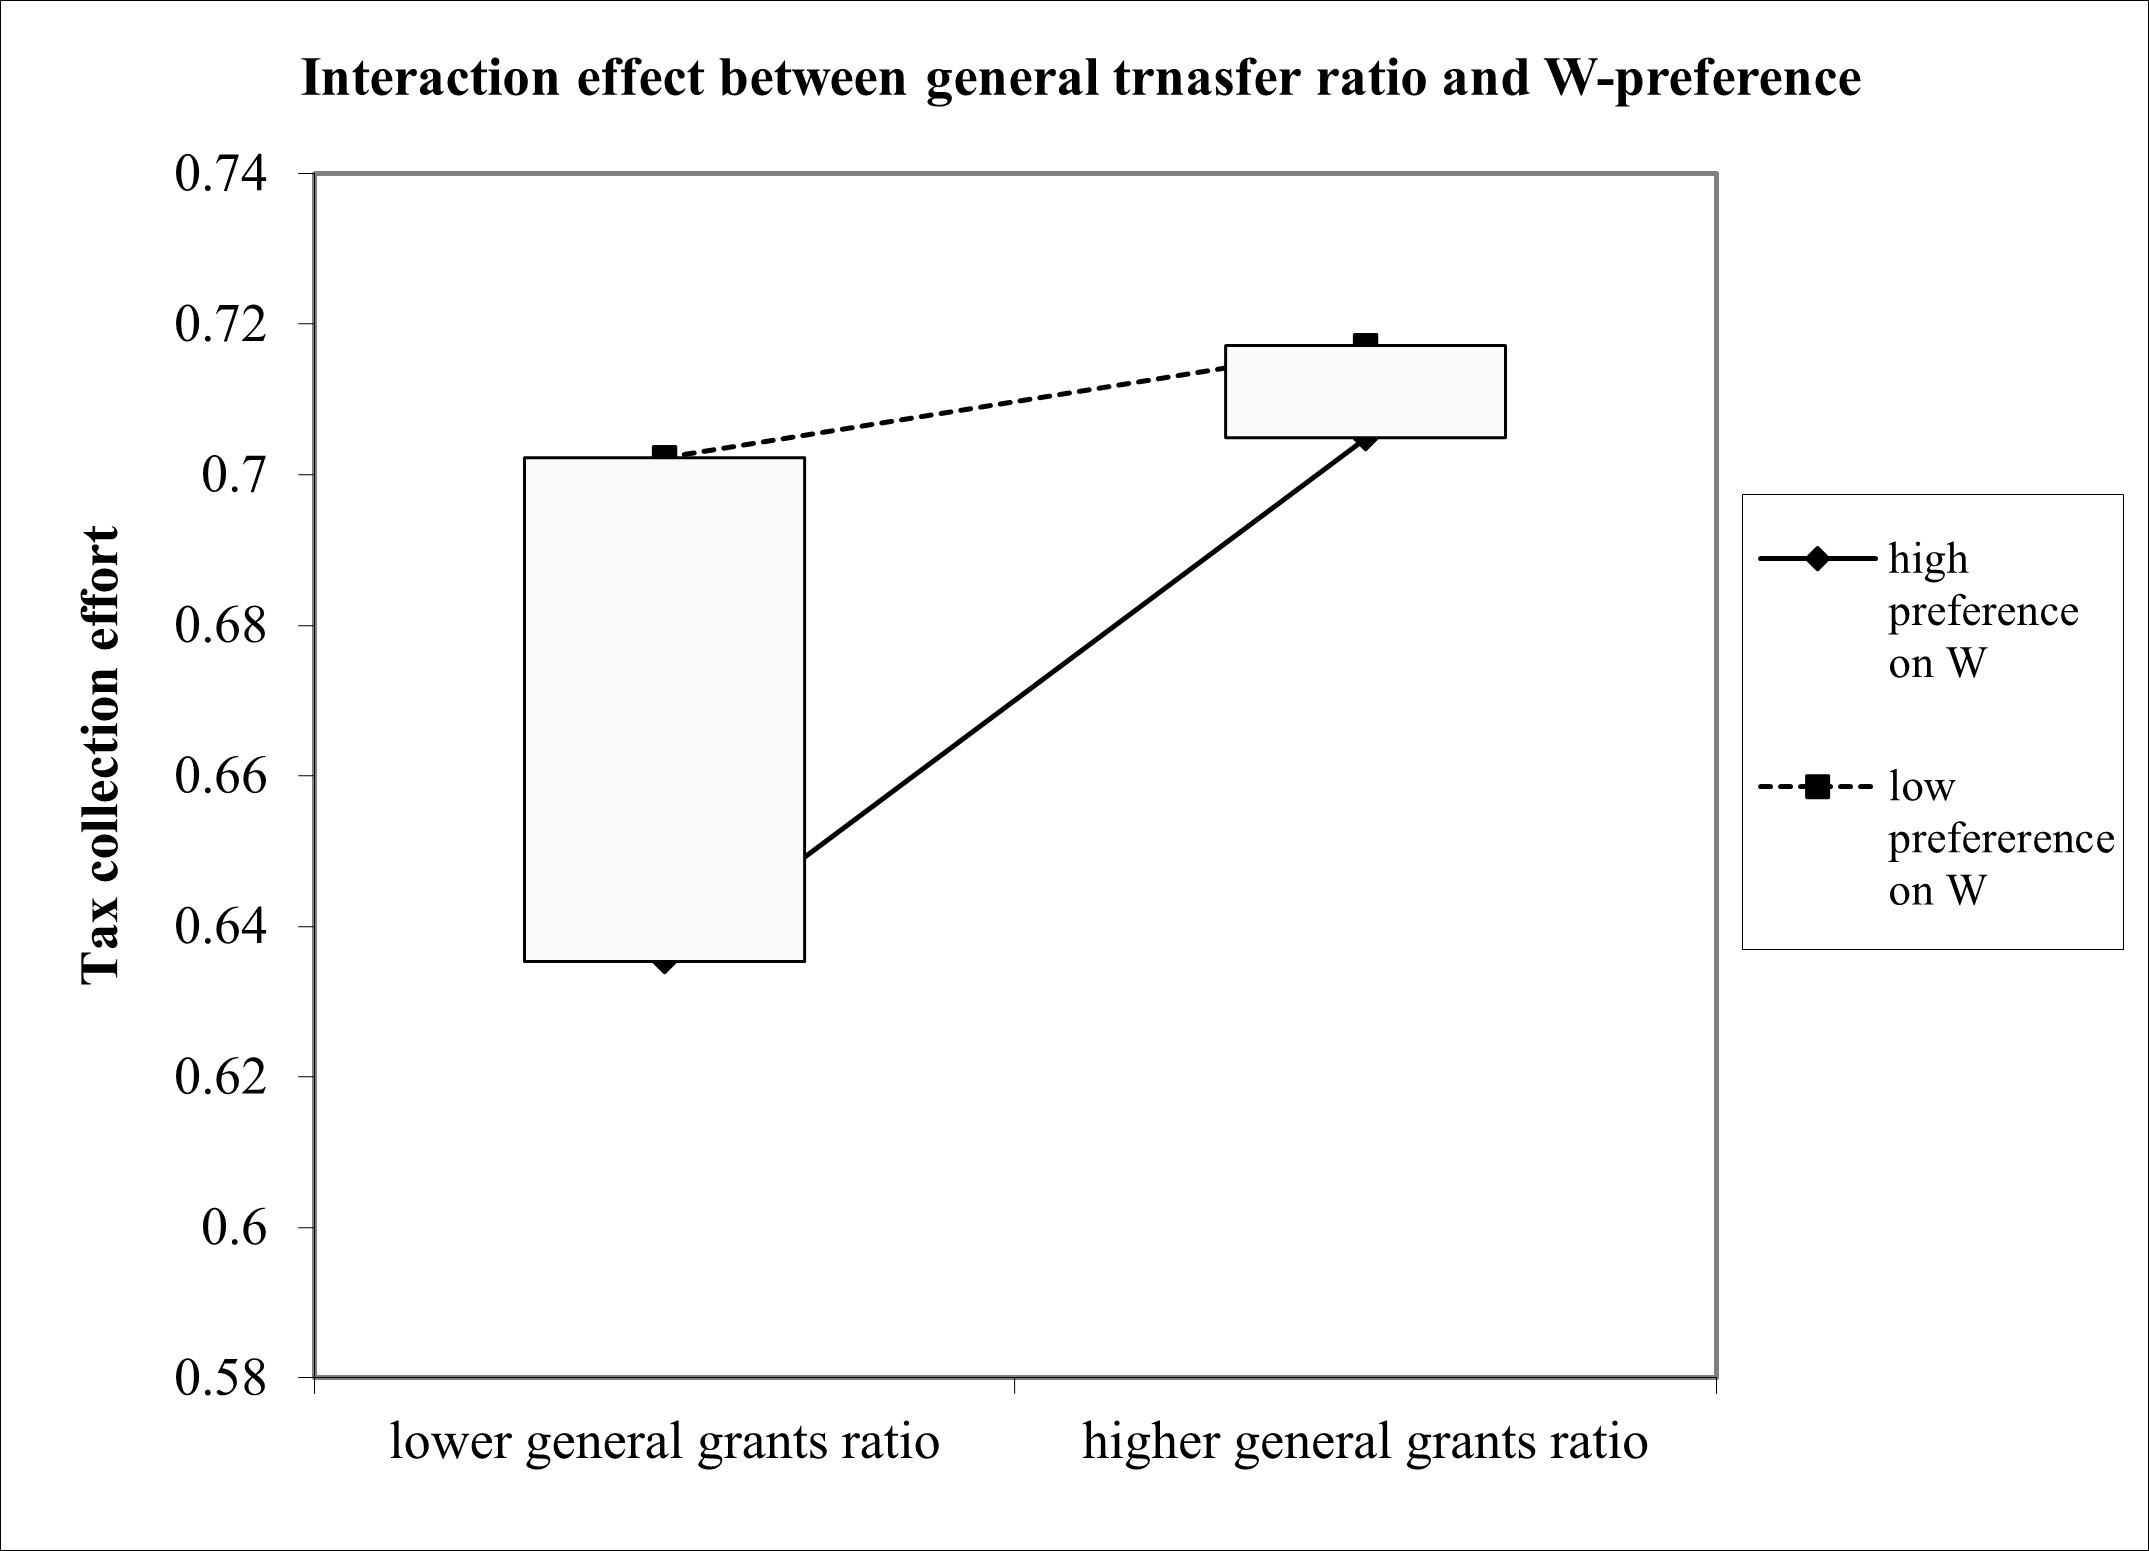
\includegraphics[scale=0.8]{Chapter-5/Figures/int_gen_W.jpg}
%     \caption[Laffer Curve for Tax Collection Effort]{Interaction effect between general trnasfer ratio and W-preference
%         \texttt{} }
%     \label{int_gen_W}
% \end{figure}

% \begin{figure}[H]
%     \centering
%     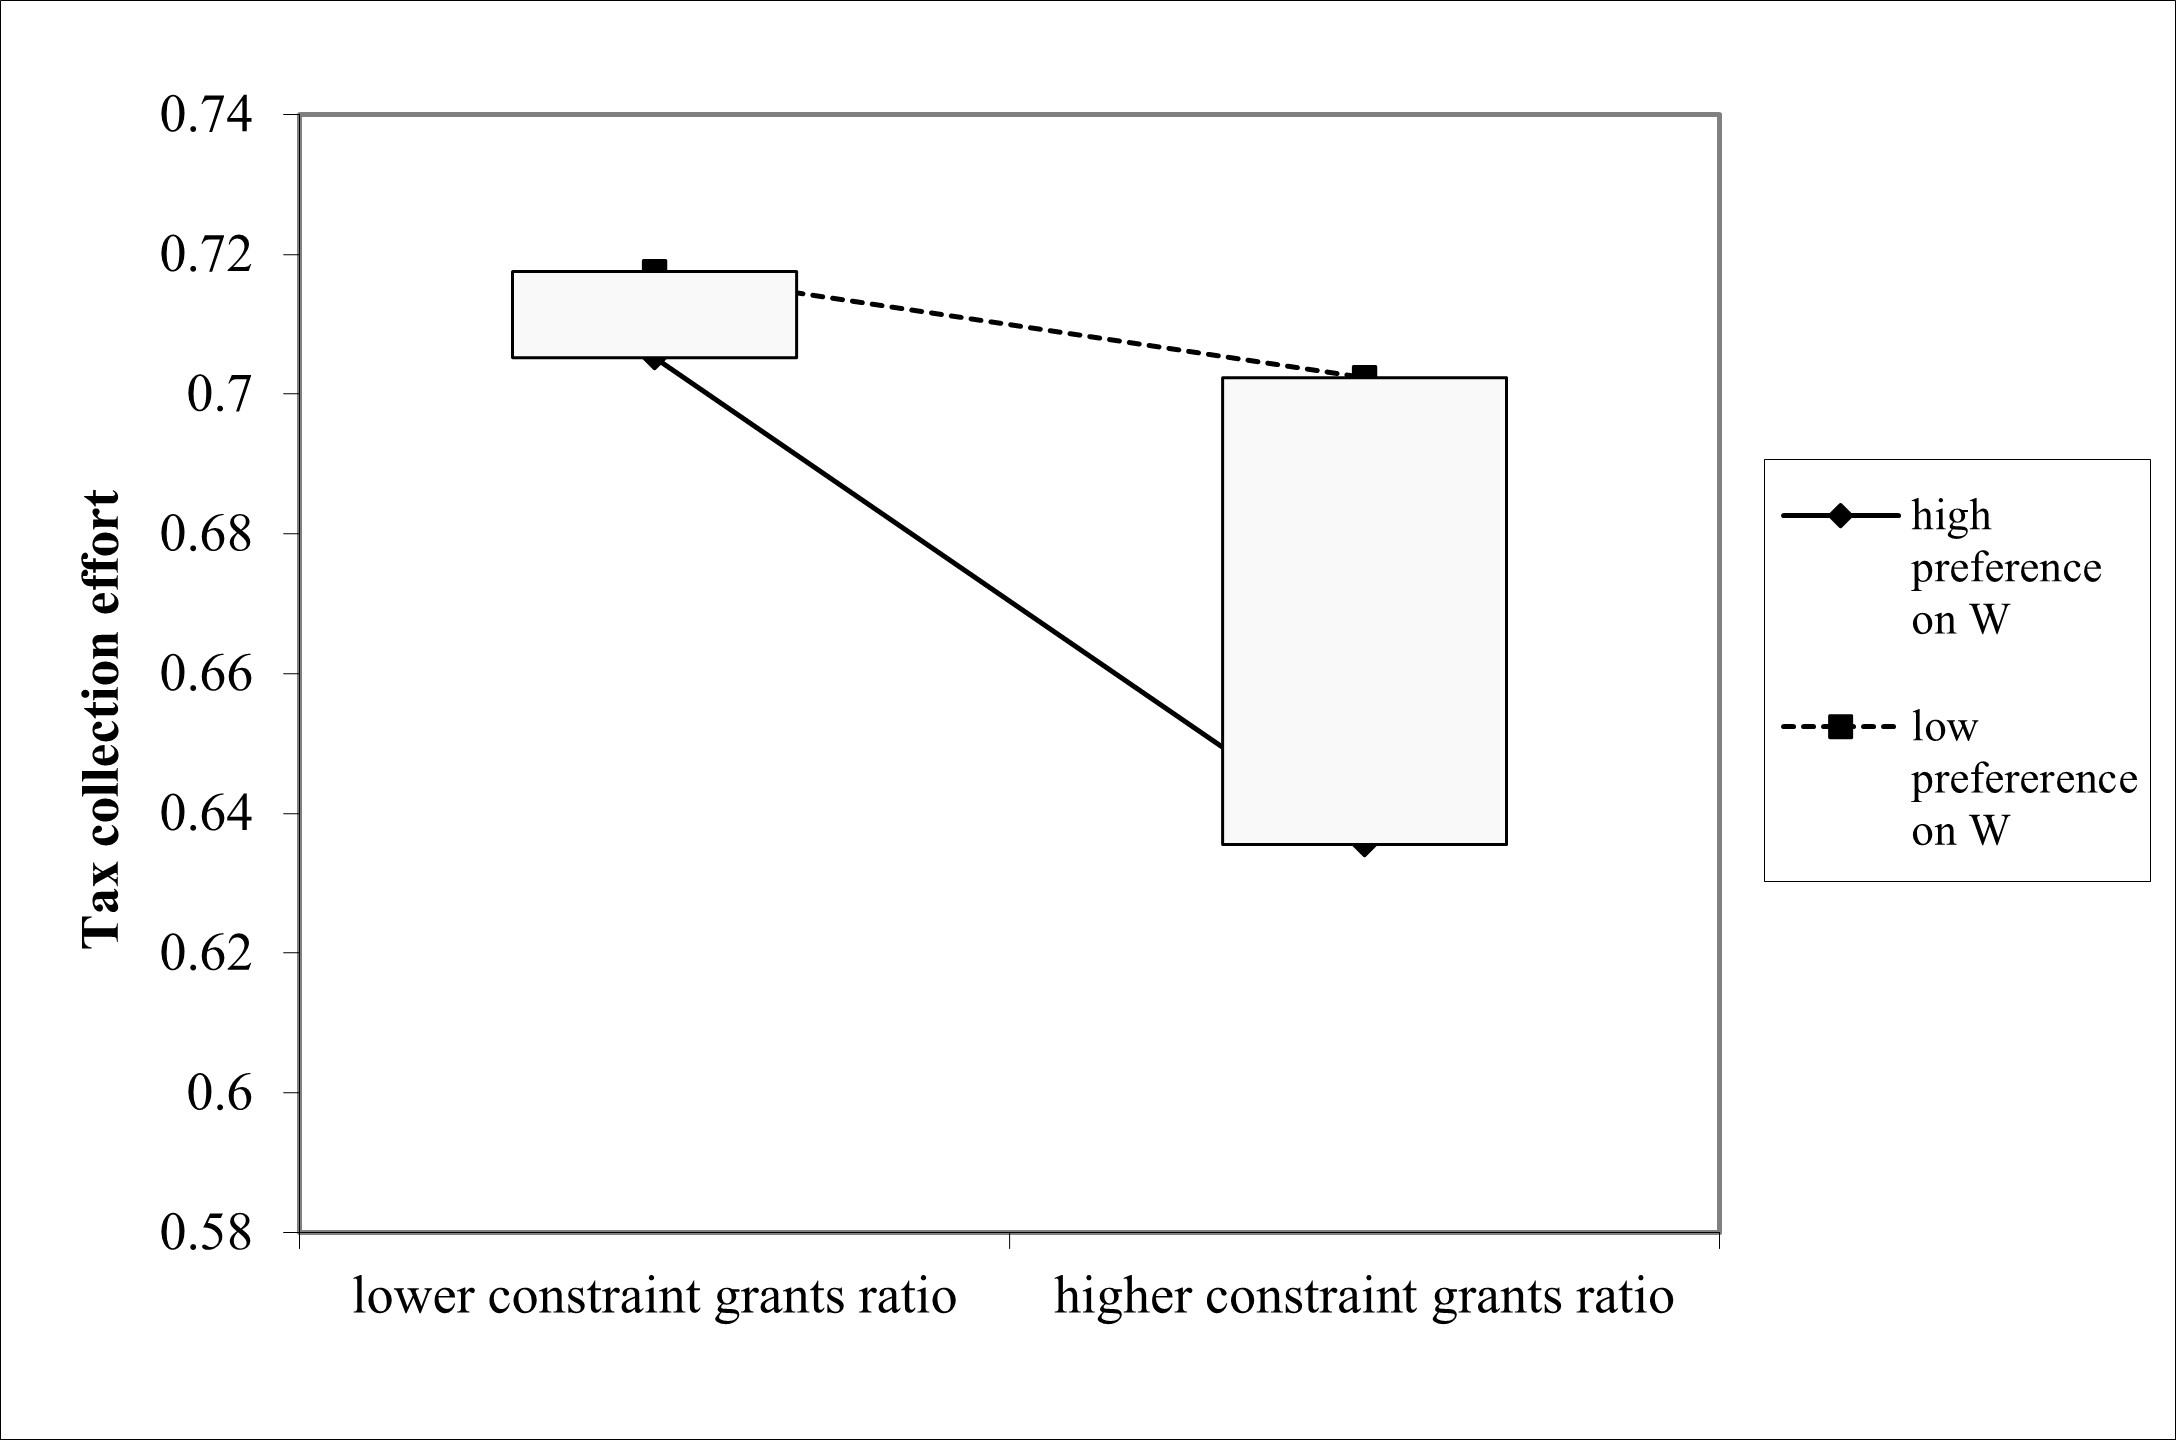
\includegraphics[scale=0.8]{Chapter-5/Figures/inter_cons_W.jpg}
%     \caption[Laffer Curve for Tax Collection Effort]{Interaction effect between welfare categorical transfer ratio and W-preference
%         \texttt{} }
%     \label{int_cons_W}
% \end{figure}

One explanation for the unexpected effect of productive categorical grants is, the effect of productive oriented grants and welfare-oriented grants could not be perfectly separated in the regression, thus the variable $constraintratio$ may not solely express productive categorical transfer. This may comes from data mixture and effect interaction. For one, we do not have an official definition about what kinds of categories of spending is considered as "productive" or "welfare". Therefore, related investigation needs to clarify the categories manually. During this process, the boundary of productive categorical transfer and welfare categorical transfer may become blurred, leading to regression results deviating from expectations. For example, \textcite{cai2005does} claims that "Infrastructure" should be interpreted broadly, including in their research that physical infrastructure (transportation, telecommunications, etc.), education, public health, and a system of well-enforced property rights and legal protections.

On the contrary, due to the relatively clear definition of general transfer payments and accurate numerical values, the econometric results align perfectly with theoretical deductions.

In addition to data mixture, another mechanism that contributes to the confounding effects of productive and welfare-specific expenditures is the diverse roles that various public investments play in economic life, which I called as interaction. For instance, social security expenditures like TANF, often perceived as purely welfare-related, also enhance the purchasing power of impoverished individuals, thereby stimulating economic growth. Similarly, public expenditures directed towards correctional facilities contribute to providing a stable and secure social environment, aiding in the reintegration of ex-convicts into society by facilitating skill development. Thus, even welfare-related expenditures may not necessarily be entirely unrelated to the overall societal output, as posited in theoretical models.


% \begin{table}[htbp]
%     \centering
%     \caption{Regression result of intergovernmental transfer on state tax collection effort}
%     \resizebox{13cm}{11cm}{
%         \begin{tabular}{ccccc}
%             \toprule
%                                         & OLS        &            & Two factors fixed effect &         \\
%             \midrule
%                                         & model-1    & model-2    & model-3                  & model-4 \\
%             \midrule
%             agrr                        & 102.6***   & 102.6***   & 19.32                    & 19.32   \\
%                                         & -15.11     & -15.11     & -1.63                    & -1.63   \\
%             minr                        & 4.513***   & 4.513***   & -2.888*                  & -2.888* \\
%                                         & -3.93      & -3.93      & (-2.20)                  & (-2.20) \\
%             manr                        & -2.163***  & -2.162***  & 0.41                     & 0.409   \\
%                                         & (-3.31)    & (-3.31)    & -0.48                    & -0.47   \\
%             infr                        & 4.669**    & 4.669**    & 1.85                     & 1.843   \\
%                                         & -2.96      & -2.96      & -0.58                    & -0.58   \\
%             fandir                      & 11.21***   & 11.21***   & 0.0485                   & 0.0543  \\
%                                         & -8.97      & -8.97      & -0.01                    & -0.02   \\
%             rer                         & 3.301***   & 3.301***   & 2.768                    & 2.766   \\
%                                         & -7.44      & -7.44      & -0.69                    & -0.68   \\
%             piepcm                      & -0.677***  & -0.677***  & -0.12                    & -0.12   \\
%                                         & (-10.67)   & (-10.67)   & (-0.89)                  & (-0.88) \\
%             mehim                       & -0.0499*** & -0.0499*** & -0.0303                  & -0.0302 \\
%                                         & (-6.14)    & (-6.14)    & (-1.28)                  & (-1.27) \\
%             unemployrate                & -0.0192*   & -0.0192*   & 0.0248                   & 0.0247  \\
%                                         & (-2.07)    & (-2.07)    & -1.59                    & -1.59   \\
%             gdppercapita                & 0.120***   & 0.120***   & 0.396                    & 0.396   \\
%                                         & -6.37      & -6.37      & -1.72                    & -1.72   \\
%             constraintratio             & -45.98*    &            & -14.38*                  &         \\
%                                         & (-2.32)    &            & (-2.56)                  &         \\
%             sw\_preference              & -9.181**   & 76.42*     & -1.806*                  & 21.61*  \\
%                                         & (-2.61)    & -2.18      & (-2.07)                  & -2.23   \\
%             int\_cons\_pref             & 70.57*     &            & 19.25*                   &         \\
%                                         & -2.22      &            & -2.22                    &         \\
%             generalratio                &            & 56.28*     &                          & 17.64*  \\
%                                         &            & -2.32      &                          & -2.57   \\
%             int\_gen\_pref              &            & -86.39*    &                          & -23.64* \\
%                                         &            & (-2.22)    &                          & (-2.23) \\
%             Constant                    & 6.760**    & -49.00*    & 2.070**                  & -15.40* \\
%                                         & -3.11      & (-2.24)    & -2.91                    & (-2.41) \\
%             \midrule
%             Observations                & 834        & 834        & 834                      & 834     \\
%             Adjusted R-sq               & 0.714      & 0.714      & 0.594                    & 0.594   \\
%             \midrule
%             t statistics in parentheses &            &            &                          &         \\
%             *p<0.05,**p<0.01,***p<0.001 &            &            &                          &         \\
%             \bottomrule
%         \end{tabular}%
%         \label{reg_igt_eff}}%
% \end{table}%


\section{Review and Summary}

This article constructs a theoretical Ramsey model based on the classification of transfer payments and the government utility function. Through solving the Ramsey model, theoretical inferences regarding the effects of general transfer and categorical transfer payments on local government tax efforts are derived. This theoretical model attempts to address two gaps in current research. Firstly, previous studies have mostly focused on discussing the impact of general transfer payments on tax efforts, with relatively fewer discussions on the role of categorical transfer, which is relatively strictly constrained. However, this article distinguishes between types of transfer payments and considers the allocation area of categorical transfer payments, thereby enabling the examination of the effects of other types of transfer payments beyond general ones. Secondly, prior research has predominantly relied on empirical tests, resulting in inconsistent conclusions on the same topic. For instance, regarding the impact of general transfer payments on tax efforts, opinions have varied between fostering and inhibiting effects. This article, through the established theoretical model, goes beyond empirical test results and discusses why the empirical evidence support divergent conclusions.

In addition to the theoretical model, this article also gathers panel data from all states in the United States from 2000 to 2019 to validate the theoretical inferences. This empirical test also innovates existing literature in two aspects. Firstly, by employing the Kalman filter, this article overcomes the difficulty of observing tax efforts and the biased proxy as substitute. Secondly, through moderating effect regression analysis, the article partially confirms the theoretical inferences.

Of course, the article also has certain limitations. Firstly, the theoretical inference regarding the impact of productive categorical transfer on tax efforts has not been empirically supported. I provided two potential reasons of the divergence, but further discussion is needed to determine whether the theoretical prediction is supported. Secondly, the article fails to provide a clear theoretical inference regarding the impact of welfare-specific transfer payments on tax efforts.

Future research in this area could focus on three main directions. Firstly, efforts could be made to improve the quality of data, particularly in accurately distinguishing between productive specific-purpose transfer payments and welfare-specific specific-purpose transfer payments during data classification. Secondly, regarding empirical testing methods, future research could explore how to accurately identify the effects of specific-purpose transfer payments in empirical tests.




% Table generated by Excel2LaTeX from sheet 'Sheet1'
% \begin{table}
%     \centering
%     \caption{Variables, measurement and data source}
%     \resizebox{\textwidth}{8cm}{
%         \begin{tabular}{c|p{11.215em}|p{6.645em}|p{6.93em}|c|c}
%             \toprule
%             \multicolumn{3}{p{24.005em}|}{Variables and Abbreviation}     & Meaning                                                       & \multicolumn{1}{p{5.715em}|}{Data Source} & \multicolumn{1}{p{5.715em}}{Time Period}                                                                                                                                                 \\
%             \midrule
%             \multicolumn{1}{c|}{\multirow{14}[28]{*}{Control Variables}}  & Agriculture                                                   & agrr                                      & \multirow{10}[20]{*}{Industrial gdp}                    & \multicolumn{1}{c|}{\multirow{10}[20]{*}{Bereau of Economic Analysis}}   & \multicolumn{1}{c}{\multirow{14}[28]{*}{2000-2019}} \\
%             \cmidrule{2-3}                                                & Mining                                                        & minr                                      & \multicolumn{1}{c|}{}                                   &                                                                          &                                                     \\
%             \cmidrule{2-3}                                                & Manufacturing                                                 & manr                                      & \multicolumn{1}{c|}{}                                   &                                                                          &                                                     \\
%             \cmidrule{2-3}                                                & Wholesale trande and Retail Trade                             & trader                                    & \multicolumn{1}{c|}{}                                   &                                                                          &                                                     \\
%             \cmidrule{2-3}                                                & Transportation and warehousing                                & tandwr                                    & \multicolumn{1}{c|}{}                                   &                                                                          &                                                     \\
%             \cmidrule{2-3}                                                & Information                                                   & infr                                      & \multicolumn{1}{c|}{}                                   &                                                                          &                                                     \\
%             \cmidrule{2-3}                                                & Finance and insurance                                         & fandir                                    & \multicolumn{1}{c|}{}                                   &                                                                          &                                                     \\
%             \cmidrule{2-3}                                                & Real estate and rental and leasing                            & rer                                       & \multicolumn{1}{c|}{}                                   &                                                                          &                                                     \\
%             \cmidrule{2-3}                                                & Health care and social assistance                             & hsr                                       & \multicolumn{1}{c|}{}                                   &                                                                          &                                                     \\
%             \cmidrule{2-3}                                                & Professional, scientific, educational, and technical services & pster                                     & \multicolumn{1}{c|}{}                                   &                                                                          &                                                     \\
%             \cmidrule{2-5}                                                & Median household income                                       & mehi                                      & \multicolumn{1}{c|}{}                                   & \multicolumn{1}{c|}{\multirow{4}[8]{*}{FRED Data Base}}                  &                                                     \\
%             \cmidrule{2-3}                                                & Unemployment rate                                             & unemployrate                              & \multicolumn{1}{c|}{}                                   &                                                                          &                                                     \\
%             \cmidrule{2-3}                                                & person income expenditure per capita                          & iepcm                                     & \multicolumn{1}{c|}{}                                   &                                                                          &                                                     \\
%             \cmidrule{2-3}                                                & GDP percapita                                                 & gdp                                       & \multicolumn{1}{c|}{}                                   &                                                                          &                                                     \\
%             \midrule
%             \multicolumn{1}{c|}{\multirow{3}[6]{*}{independent variable}} & Welfare spending preference                                   & w\_preference                             & Welfare preferernce of federal and state government     & \multicolumn{1}{c|}{\multirow{3}[6]{*}{State Expenditure Annual Report}} & \multicolumn{1}{c}{\multirow{3}[6]{*}{2000-2019}}   \\
%             \cmidrule{2-4}                                                & general ratio                                                 & gen\_ratio                                & Federal grants ratio with no constraints                &                                                                          &                                                     \\
%             \cmidrule{2-4}                                                & productive spending matching ratio                            & cons\_ratio                               & Federal categorical grants ratio on productive spending &                                                                          &                                                     \\
%             \bottomrule
%         \end{tabular}}%
%     \label{datasource}%
% \end{table}%
% % Table generated by Excel2LaTeX from sheet 'xtregionolsss0212'

    % \chapter{How to Explain  the Difference between the Asymmetric Behavior between central and local government.}

\section{How to Explain the Fly Paper Effect}


\section{What May be the Impact on the Supply of Public Goods of Local Government}

    %%%%%%%%%%%%%%%%%%%%%%%%%%%%%%%%%%%%%%%%%%%%%%%%%%%%%%%%%%%%%%%
    % Appendices
    %
    % Because of a quirk in LaTeX (see p. 48 of The LaTeX
    % Companion, 2e), you cannot use \include along with
    % \addtocontents if you want things to appear the proper
    % sequence.
    %%%%%%%%%%%%%%%%%%%%%%%%%%%%%%%%%%%%%%%%%%%%%%%%%%%%%%%%%%%%%%%
    \appendix
    \titleformat{\chapter}[display]{\fontsize{30}{30}\selectfont\bfseries\sffamily}{Appendix \thechapter\textcolor{gray75}{\raisebox{3pt}{|}}}{0pt}{}{}
    % If you have a single appendix, then to prevent LaTeX from
    % calling it ``Appendix A'', you should uncomment the following two
    % lines that redefine the \thechapter and \thesection:
    %\renewcommand\thechapter{}
    %\renewcommand\thesection{\arabic{section}}
    % !TEX root = ../YourName-Dissertation.tex
\Appendix{Supportive Data and Figures}

\section{Data}
% Table generated by Excel2LaTeX from sheet 'Sheet1'
\begin{table}[htbp]
  \centering
  \caption{Data Source and operation for the empirical test in Section 2.3.3}
  \begin{tabular}{ccp{8.785em}c}
    \toprule
    \multicolumn{2}{p{13.93em}}{Variables }                                         & Source  & \multicolumn{1}{p{7.785em}}{Time Period}                                                                         \\
    \midrule
    \multicolumn{1}{p{7em}}{Dependent Variable}                                     & lg(igt) & State CAFR                               & \multicolumn{1}{c}{\multirow{9}[18]{*}{2000-2019 annually collected}} \\
    \cmidrule{1-3}    \multicolumn{1}{c}{\multirow{2}[4]{*}{Independent Variables}} & c       & \multirow{2}[4]{*}{Ballotpedia}          &                                                                       \\
    \cmidrule{2-2}                                                                  & p       & \multicolumn{1}{c}{}                     &                                                                       \\
    \cmidrule{1-3}    \multicolumn{1}{c}{\multirow{6}[12]{*}{Control Variables}}    & gdp     & FRED                                     &                                                                       \\
    \cmidrule{2-3}                                                                  & lgp     & \multirow{4}[8]{*}{Census of bureau}     &                                                                       \\
    \cmidrule{2-2}                                                                  & wapw    & \multicolumn{1}{c}{}                     &                                                                       \\
    \cmidrule{2-2}                                                                  & mhi     & \multicolumn{1}{c}{}                     &                                                                       \\
    \cmidrule{2-2}                                                                  & ur      & \multicolumn{1}{c}{}                     &                                                                       \\
    \cmidrule{2-3}                                                                  & prm     & Bureau of transportation statistics      &                                                                       \\
    \bottomrule
  \end{tabular}%
  \label{Table A.1}%
\end{table}%


\section{Figures}
%%%
%%%%%%%%%%%%%%%%%%%%%%%%%%%%%%%%%%
\begin{figure}[H]
  \centering  %居中
  \subfigure[Federal Expenditure]{   %first subfigure
    \begin{minipage}{7cm}
      \centering    %子图居中
      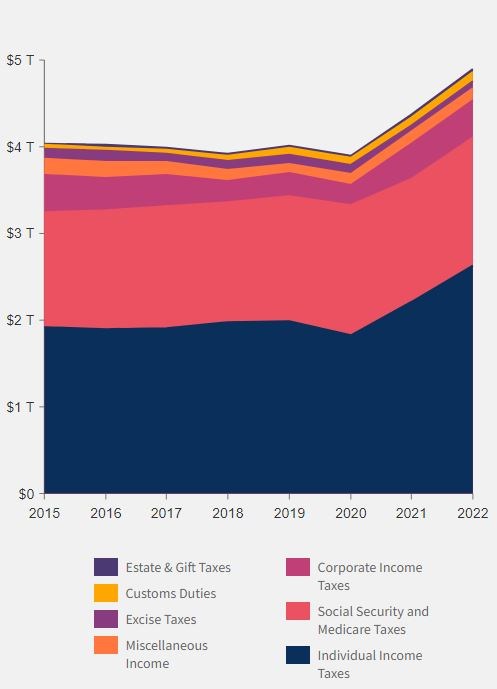
\includegraphics[scale=0.52]{Chapter-1/Figures/source of federal revenue.JPG}  %以pic.jpg的0.5倍大小输出
    \end{minipage}
  }
  \subfigure[State and Local Expenditure]{ %second subfigure
    \begin{minipage}{7cm}
      \centering    %子图居中
      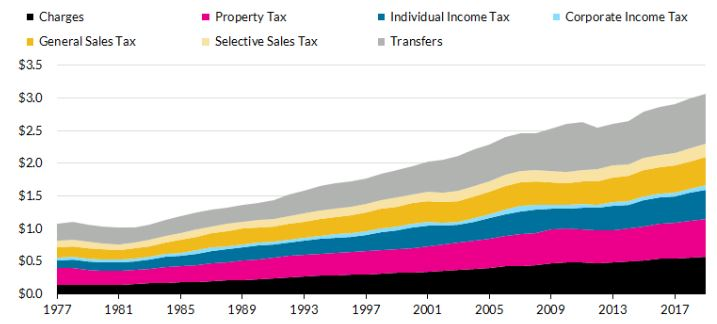
\includegraphics[scale=0.52]{Chapter-1/Figures/source of state and local revenue.JPG}%以pic.jpg的0.5倍大小输出
    \end{minipage}
  }

  \caption[Fluctuation of Revenue Structure]{Fluctuation of Revenue Structure of three level governments.Data Source: US Urban Institute Dataset  }    %caption for whole figure
  \label{Figure A.1}
\end{figure}

%%%%%%%%%%%%%%%%%%%%%%%%%%%%%%%%%%%%%%%%%%%%%%%

\begin{figure}[H]
  \centering
  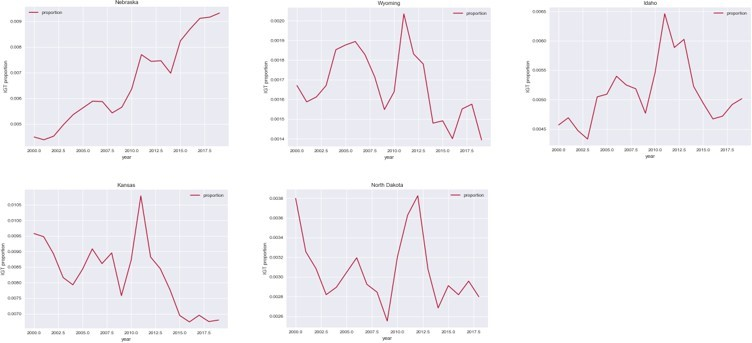
\includegraphics[scale=0.7]{Appendix-A/republican.jpg}
  \caption[Time Series Graph of Republican States IGT (2000-2019)]{Time Series Graph of Republican States IGT (2000-2019)
    \texttt{} }
  \label{Figure A.2}
\end{figure}

\begin{figure}[H]
  \centering
  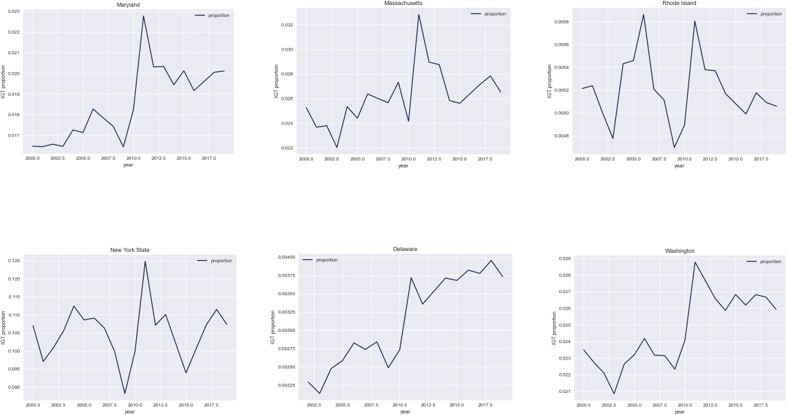
\includegraphics[scale=0.7]{Appendix-A/democratic.jpg}
  \caption[Time Series Graph of Democratic States IGT(2000-2019)]{Time Series Graph of Democratic States IGT (2000-2019)
    \texttt{} }
  \label{Figure A.3}
\end{figure}

\begin{figure}[H]
  \centering
  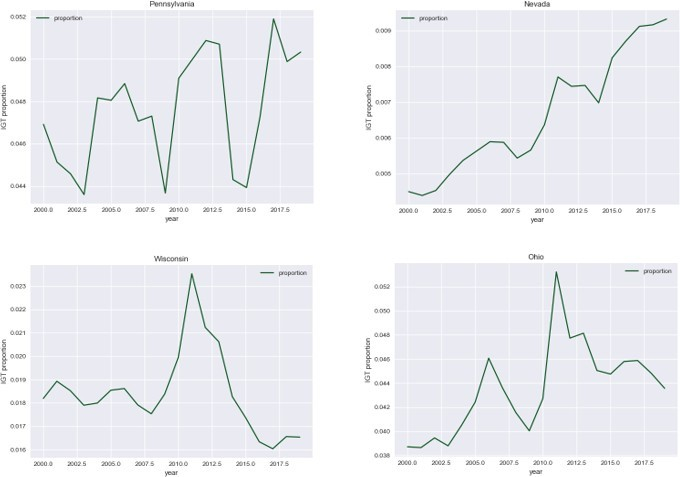
\includegraphics[scale=0.7]{Appendix-A/swing.jpg}
  \caption[Time Series Graph of Swing States IGT (2000-2019) ]{Time Series Graph of Swing States IGT (2000-2019)
    \texttt{} }
  \label{Figure A.4}
\end{figure}

    % !TEX root = ../YourName-Dissertation.tex
\Appendix{Figures}

\section{Chapter 1}
\begin{figure}[H]
    \centering
    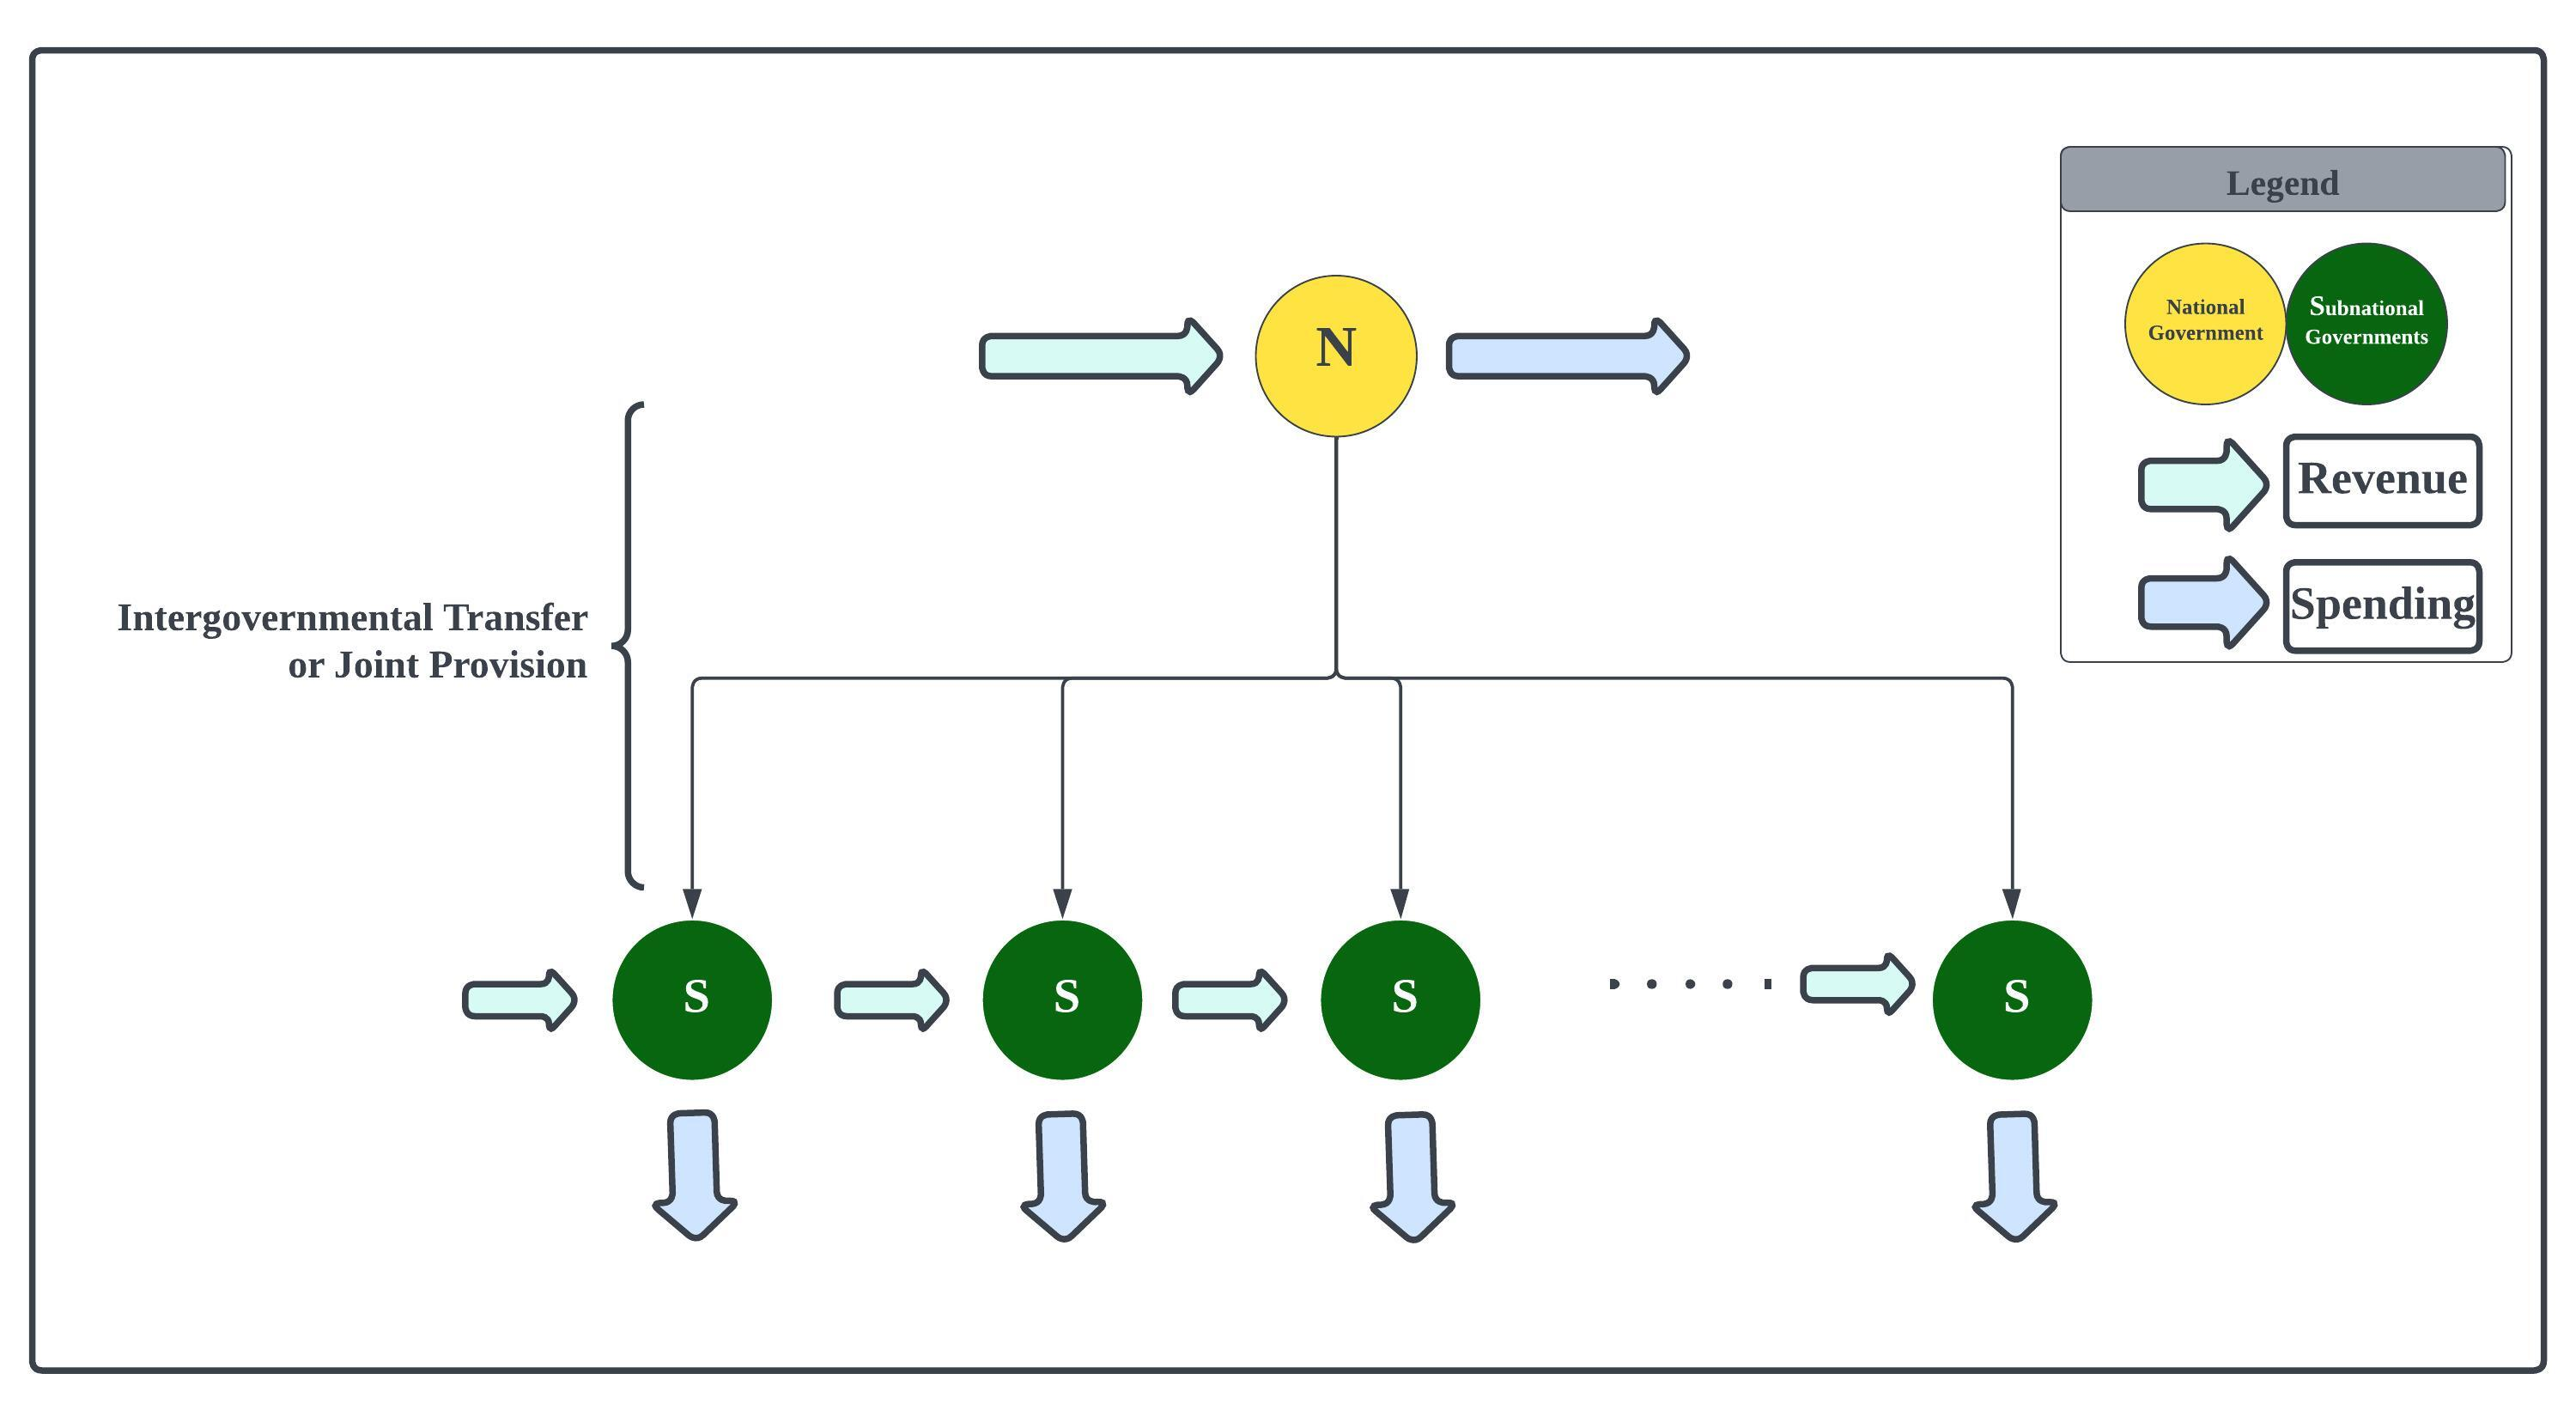
\includegraphics[scale=0.6]{Chapter-1/Figures/fiscal federalism.jpeg}
    \caption[Fiscal Federalism Structure]{Fiscal Federalism Structure
        \texttt{} }
    \label{Figure 1.1}
\end{figure}

\clearpage

\begin{figure}[H]
    \centering  %居中
    \subfigure[Federal Expenditure]{   %first subfigure
        \begin{minipage}{7cm}
            \centering    %子图居中
            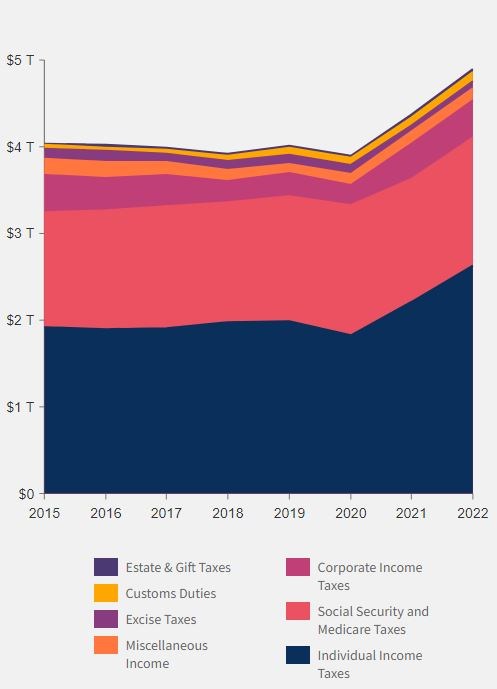
\includegraphics[scale=0.52]{Chapter-1/Figures/source of federal revenue.JPG}  %以pic.jpg的0.5倍大小输出
        \end{minipage}
    }
    \subfigure[State and Local Expenditure]{ %second subfigure
        \begin{minipage}{7cm}
            \centering    %子图居中
            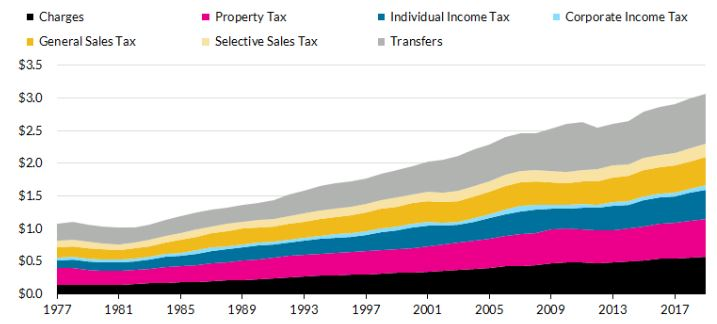
\includegraphics[scale=0.52]{Chapter-1/Figures/source of state and local revenue.JPG}%以pic.jpg的0.5倍大小输出
        \end{minipage}
    }

    \caption[Fluctuation of Revenue Structure]{Fluctuation of Revenue Structure of three level governments.Data Source: US Urban Institute Dataset  }    %caption for whole figure
    \label{Figure A.1}
\end{figure}

\clearpage

\begin{figure}[H]
    \centering
    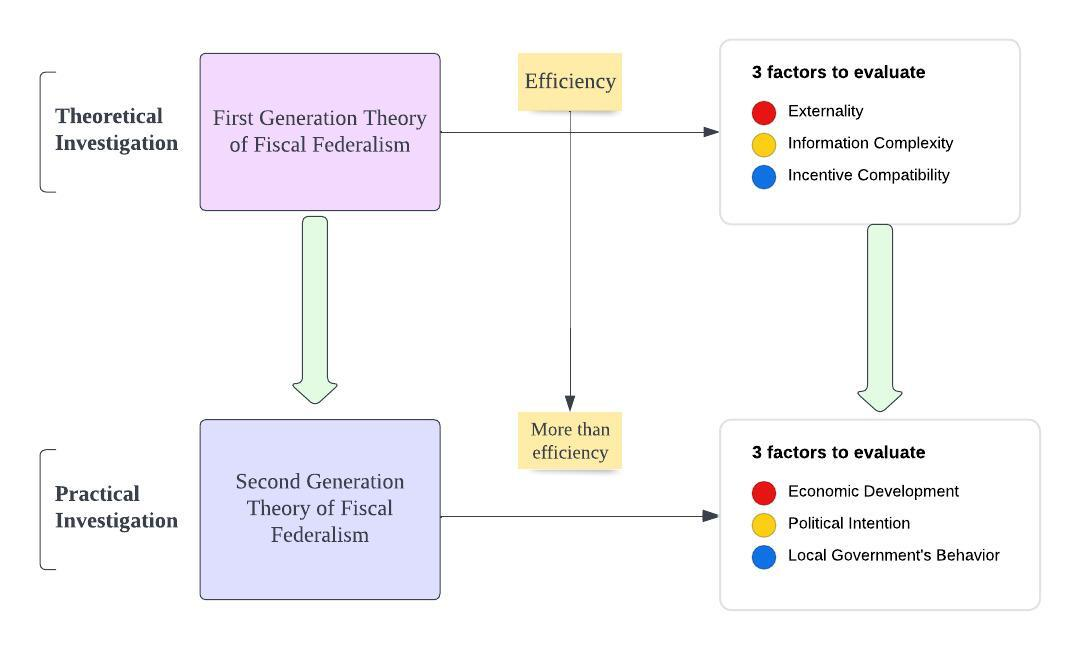
\includegraphics[scale=1]{Chapter-2/Figures/how to evaluate the fiscal federalism.jpeg}
    \caption[How to evaluate the fiscal federalism]{How to evaluate the fiscal federalism
        \texttt{} }
    \label{Figure 1.2}
\end{figure}

\clearpage

\begin{figure}[htbp]
    \centering
    \subfigure[Source of Federal Revenue]{
        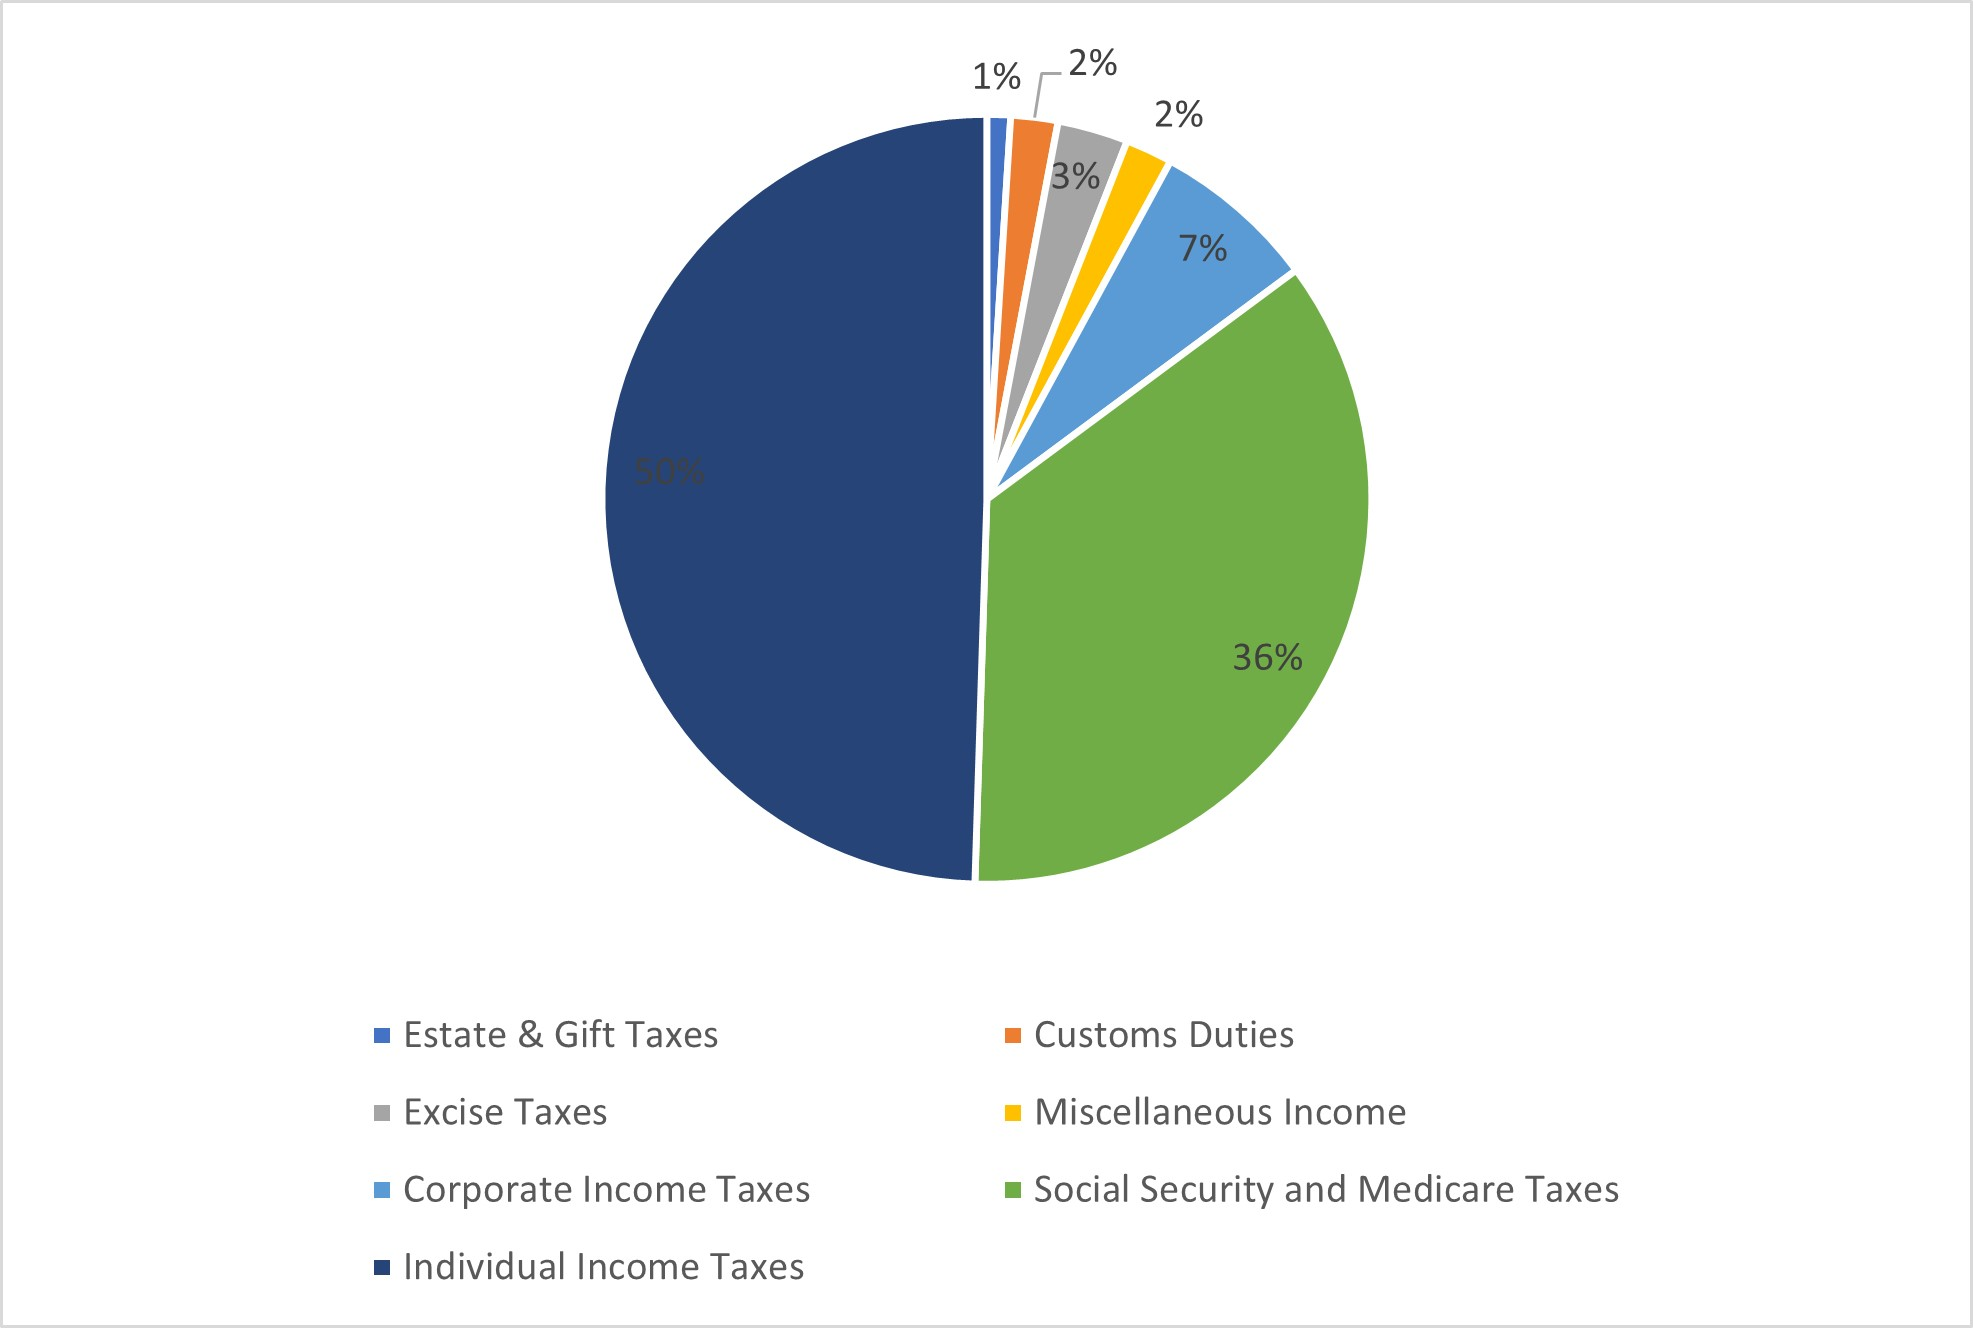
\includegraphics[width=0.31\textwidth]{Chapter-1/Figures/source of federal general revenue.jpg}}
    \subfigure[Source of State Revenue]{
        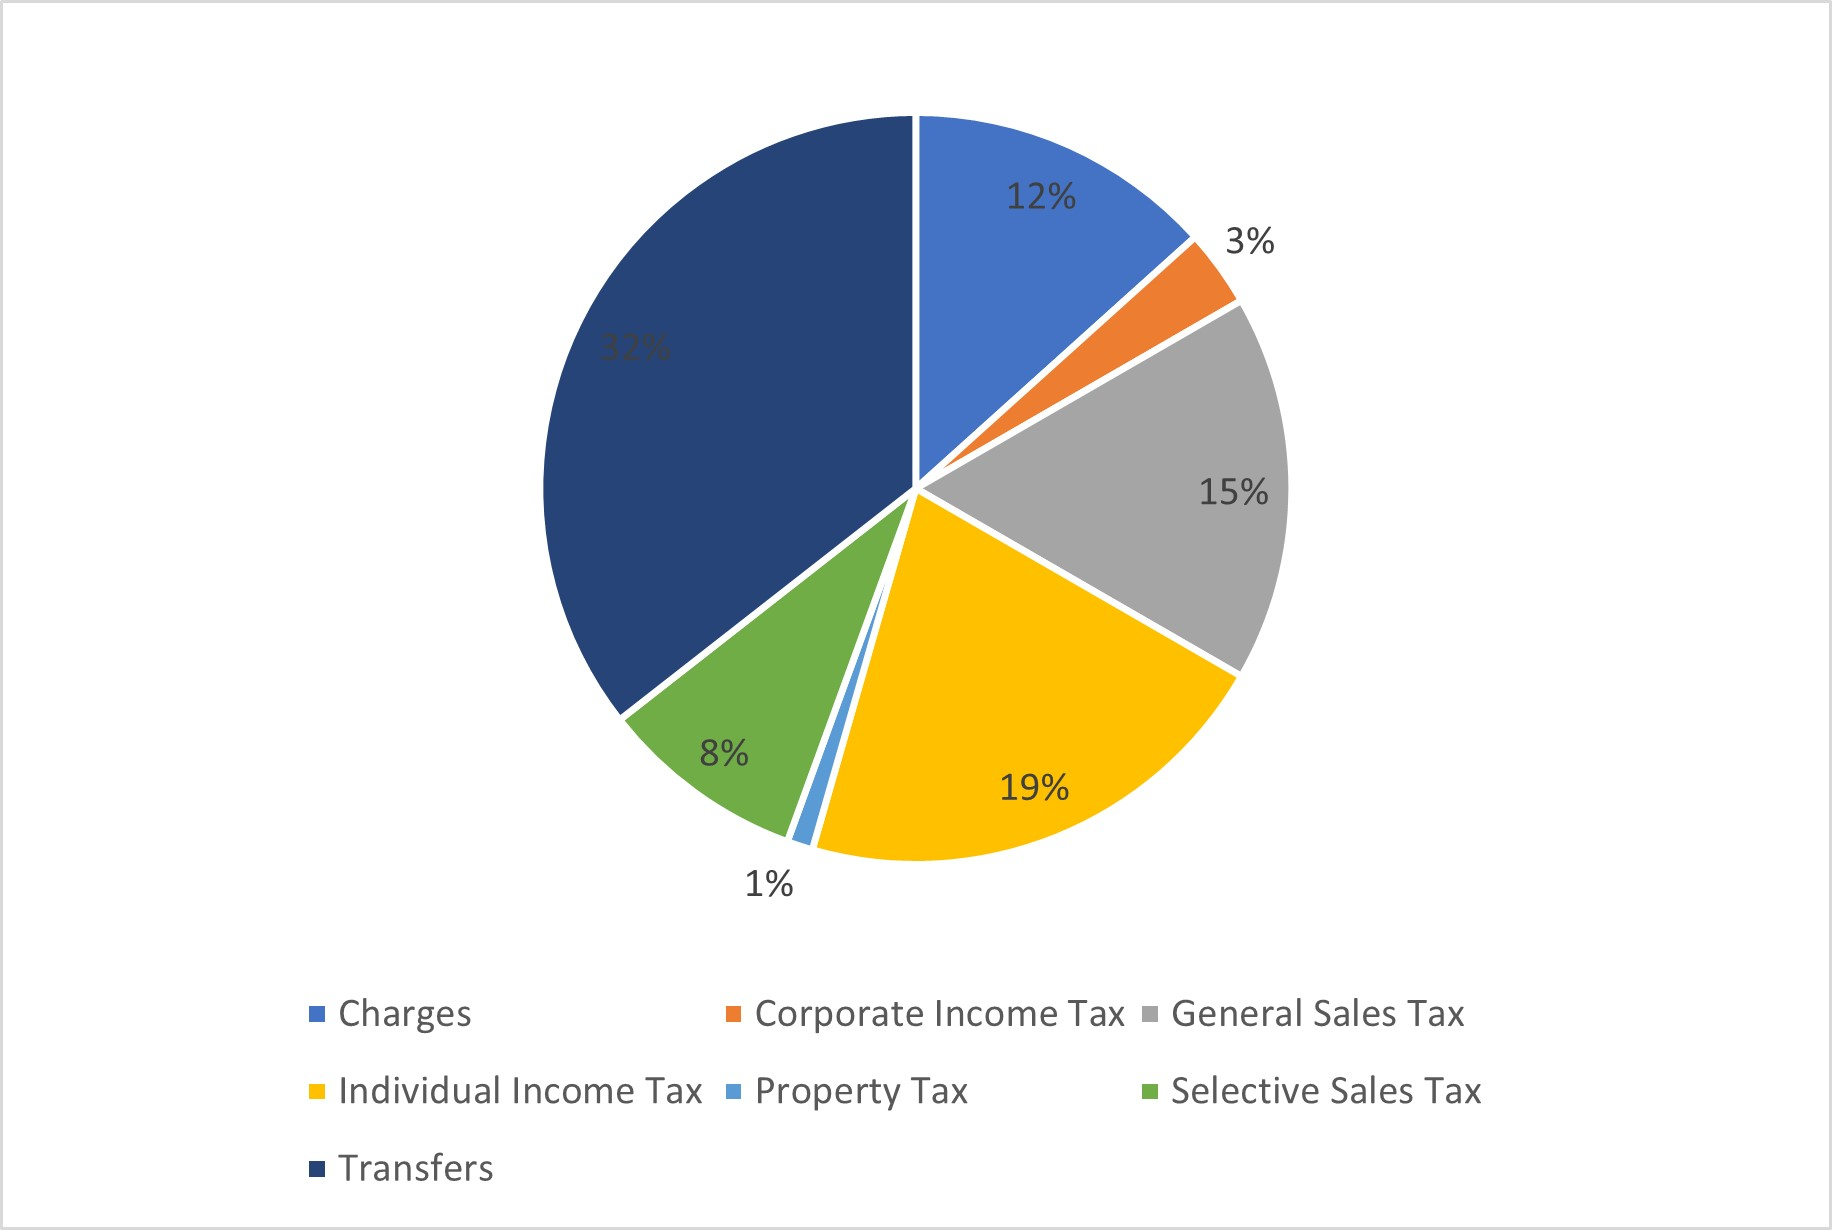
\includegraphics[width=0.31\textwidth]{Chapter-1/Figures/source of state general revenue.jpg}}
    \subfigure[Source of Local Revenue]{
        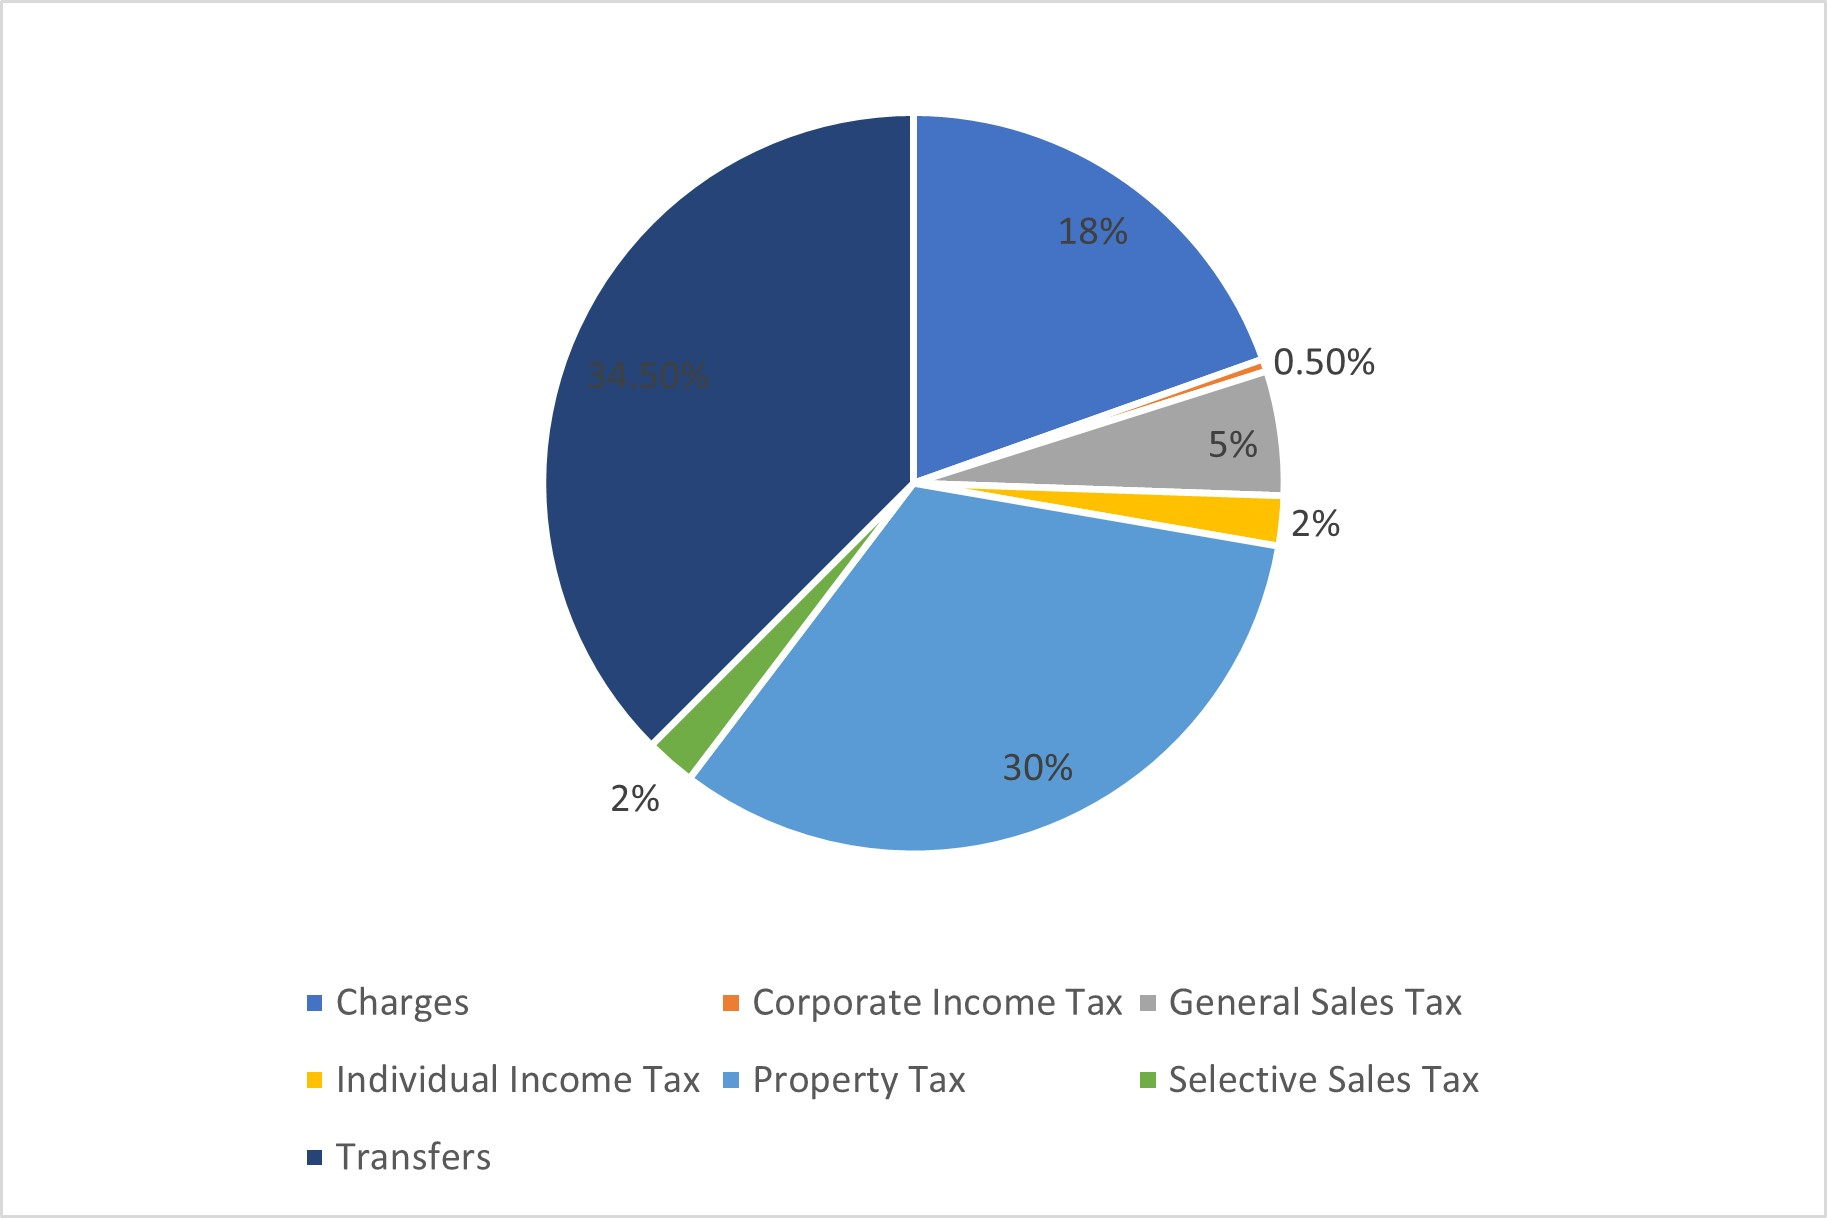
\includegraphics[width=0.31\textwidth]{Chapter-1/Figures/sources of local general revenue.jpg}}
    \caption[Source of Revenue for Multiple Level of Governments in 2019]
    {Source of Revenue for Multiple Level of Governments}
    \label{sourceofreveune}
\end{figure}

\begin{figure}[H]
    \centering  %居中
    \subfigure[Federal Expenditure]{   %first subfigure
        \begin{minipage}{7cm}
            \centering    %子图居中
            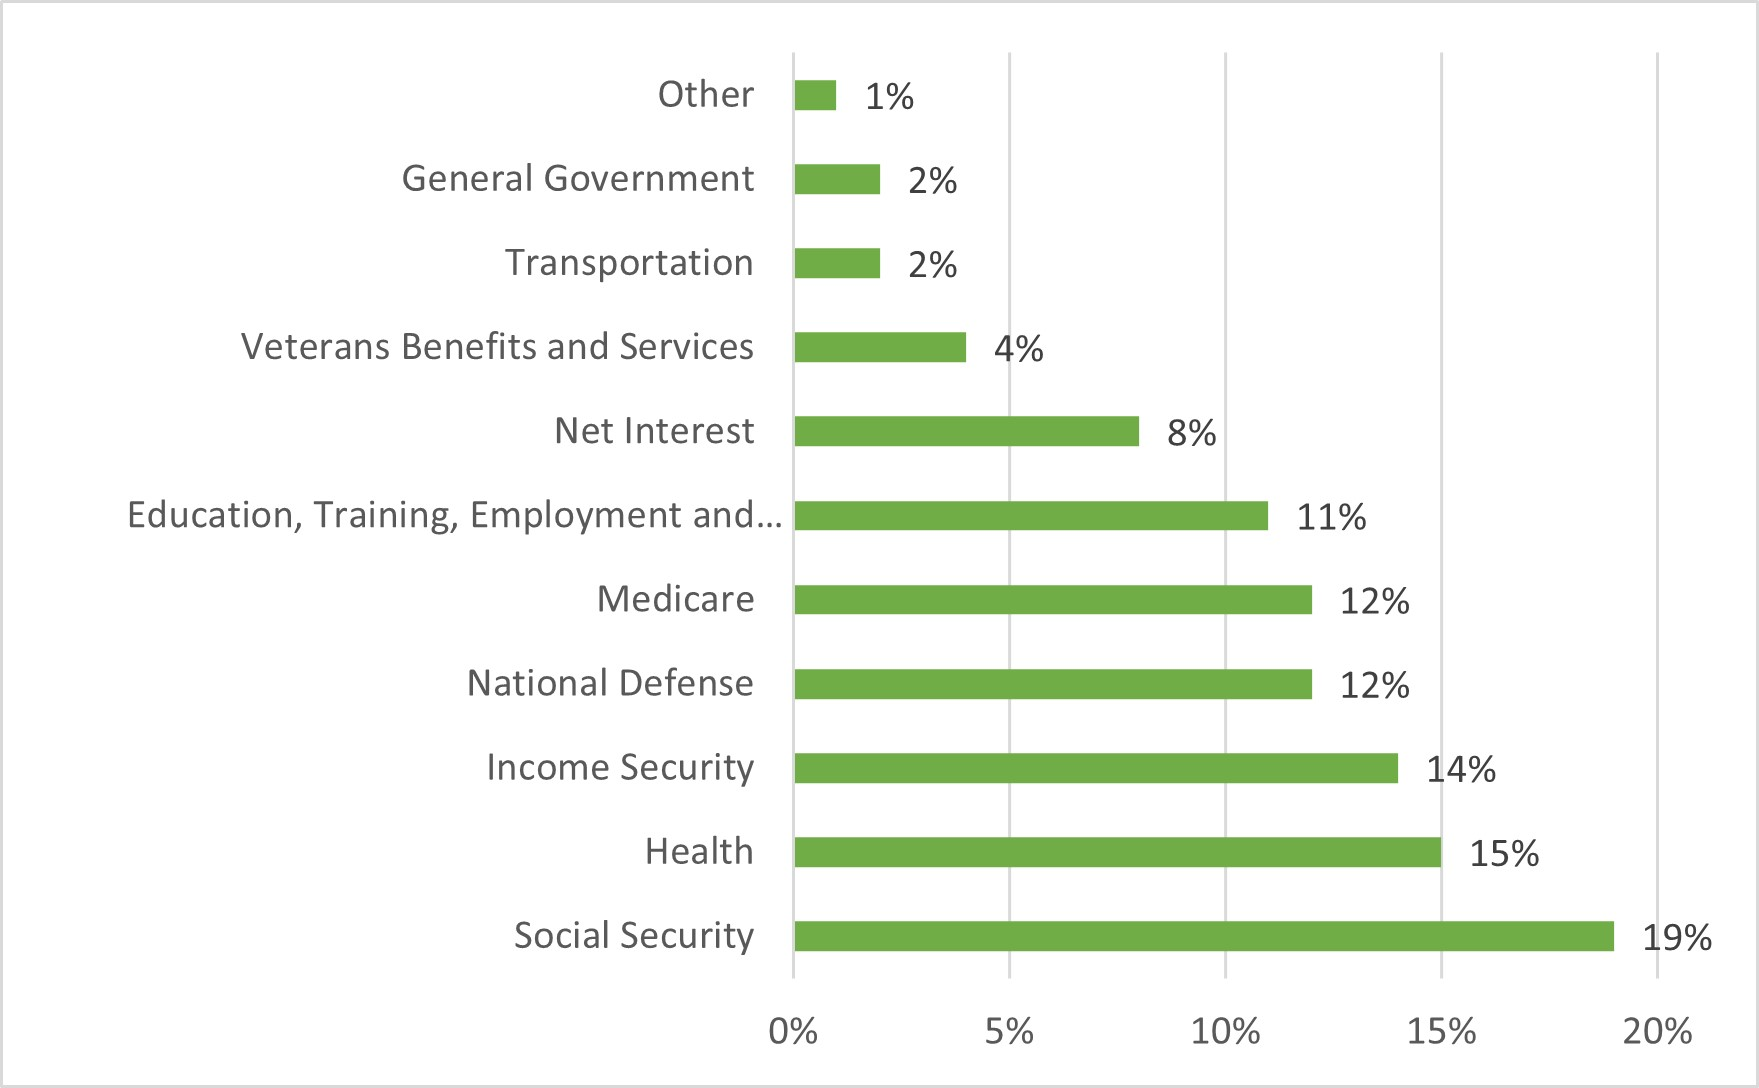
\includegraphics[scale=0.52]{Chapter-1/Figures/federal expenditure.JPG}  %以pic.jpg的0.5倍大小输出
        \end{minipage}
    }
    \subfigure[State and Local Expenditure]{ %second subfigure
        \begin{minipage}{7cm}
            \centering    %子图居中
            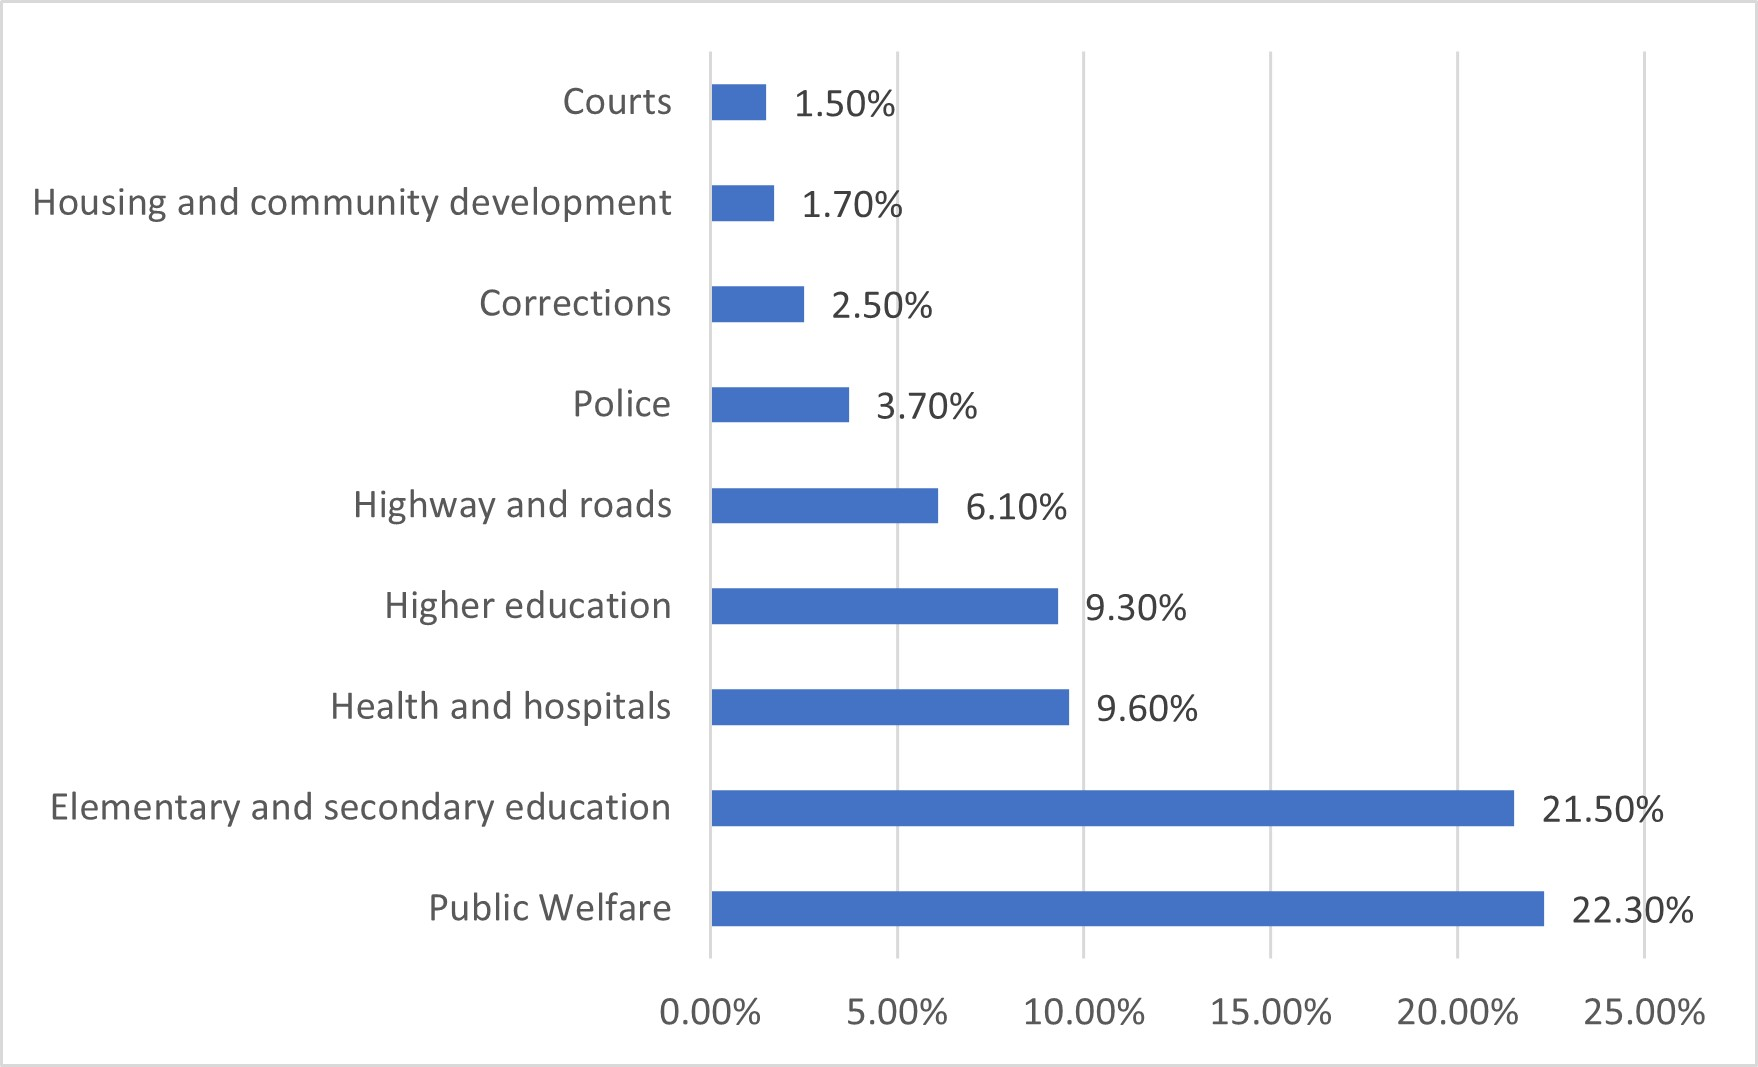
\includegraphics[scale=0.52]{Chapter-1/Figures/state and local expenditure.JPG}%以pic.jpg的0.5倍大小输出
        \end{minipage}
    }

    \caption[Expenditure Structure for Multiple Level of Governments in 2019]{Expenditure Structure for Multiple Level of Governments.}    %caption for whole figure
    \label{Figure 1.3}
\end{figure}
\clearpage

\begin{figure}[H]
    \centering
    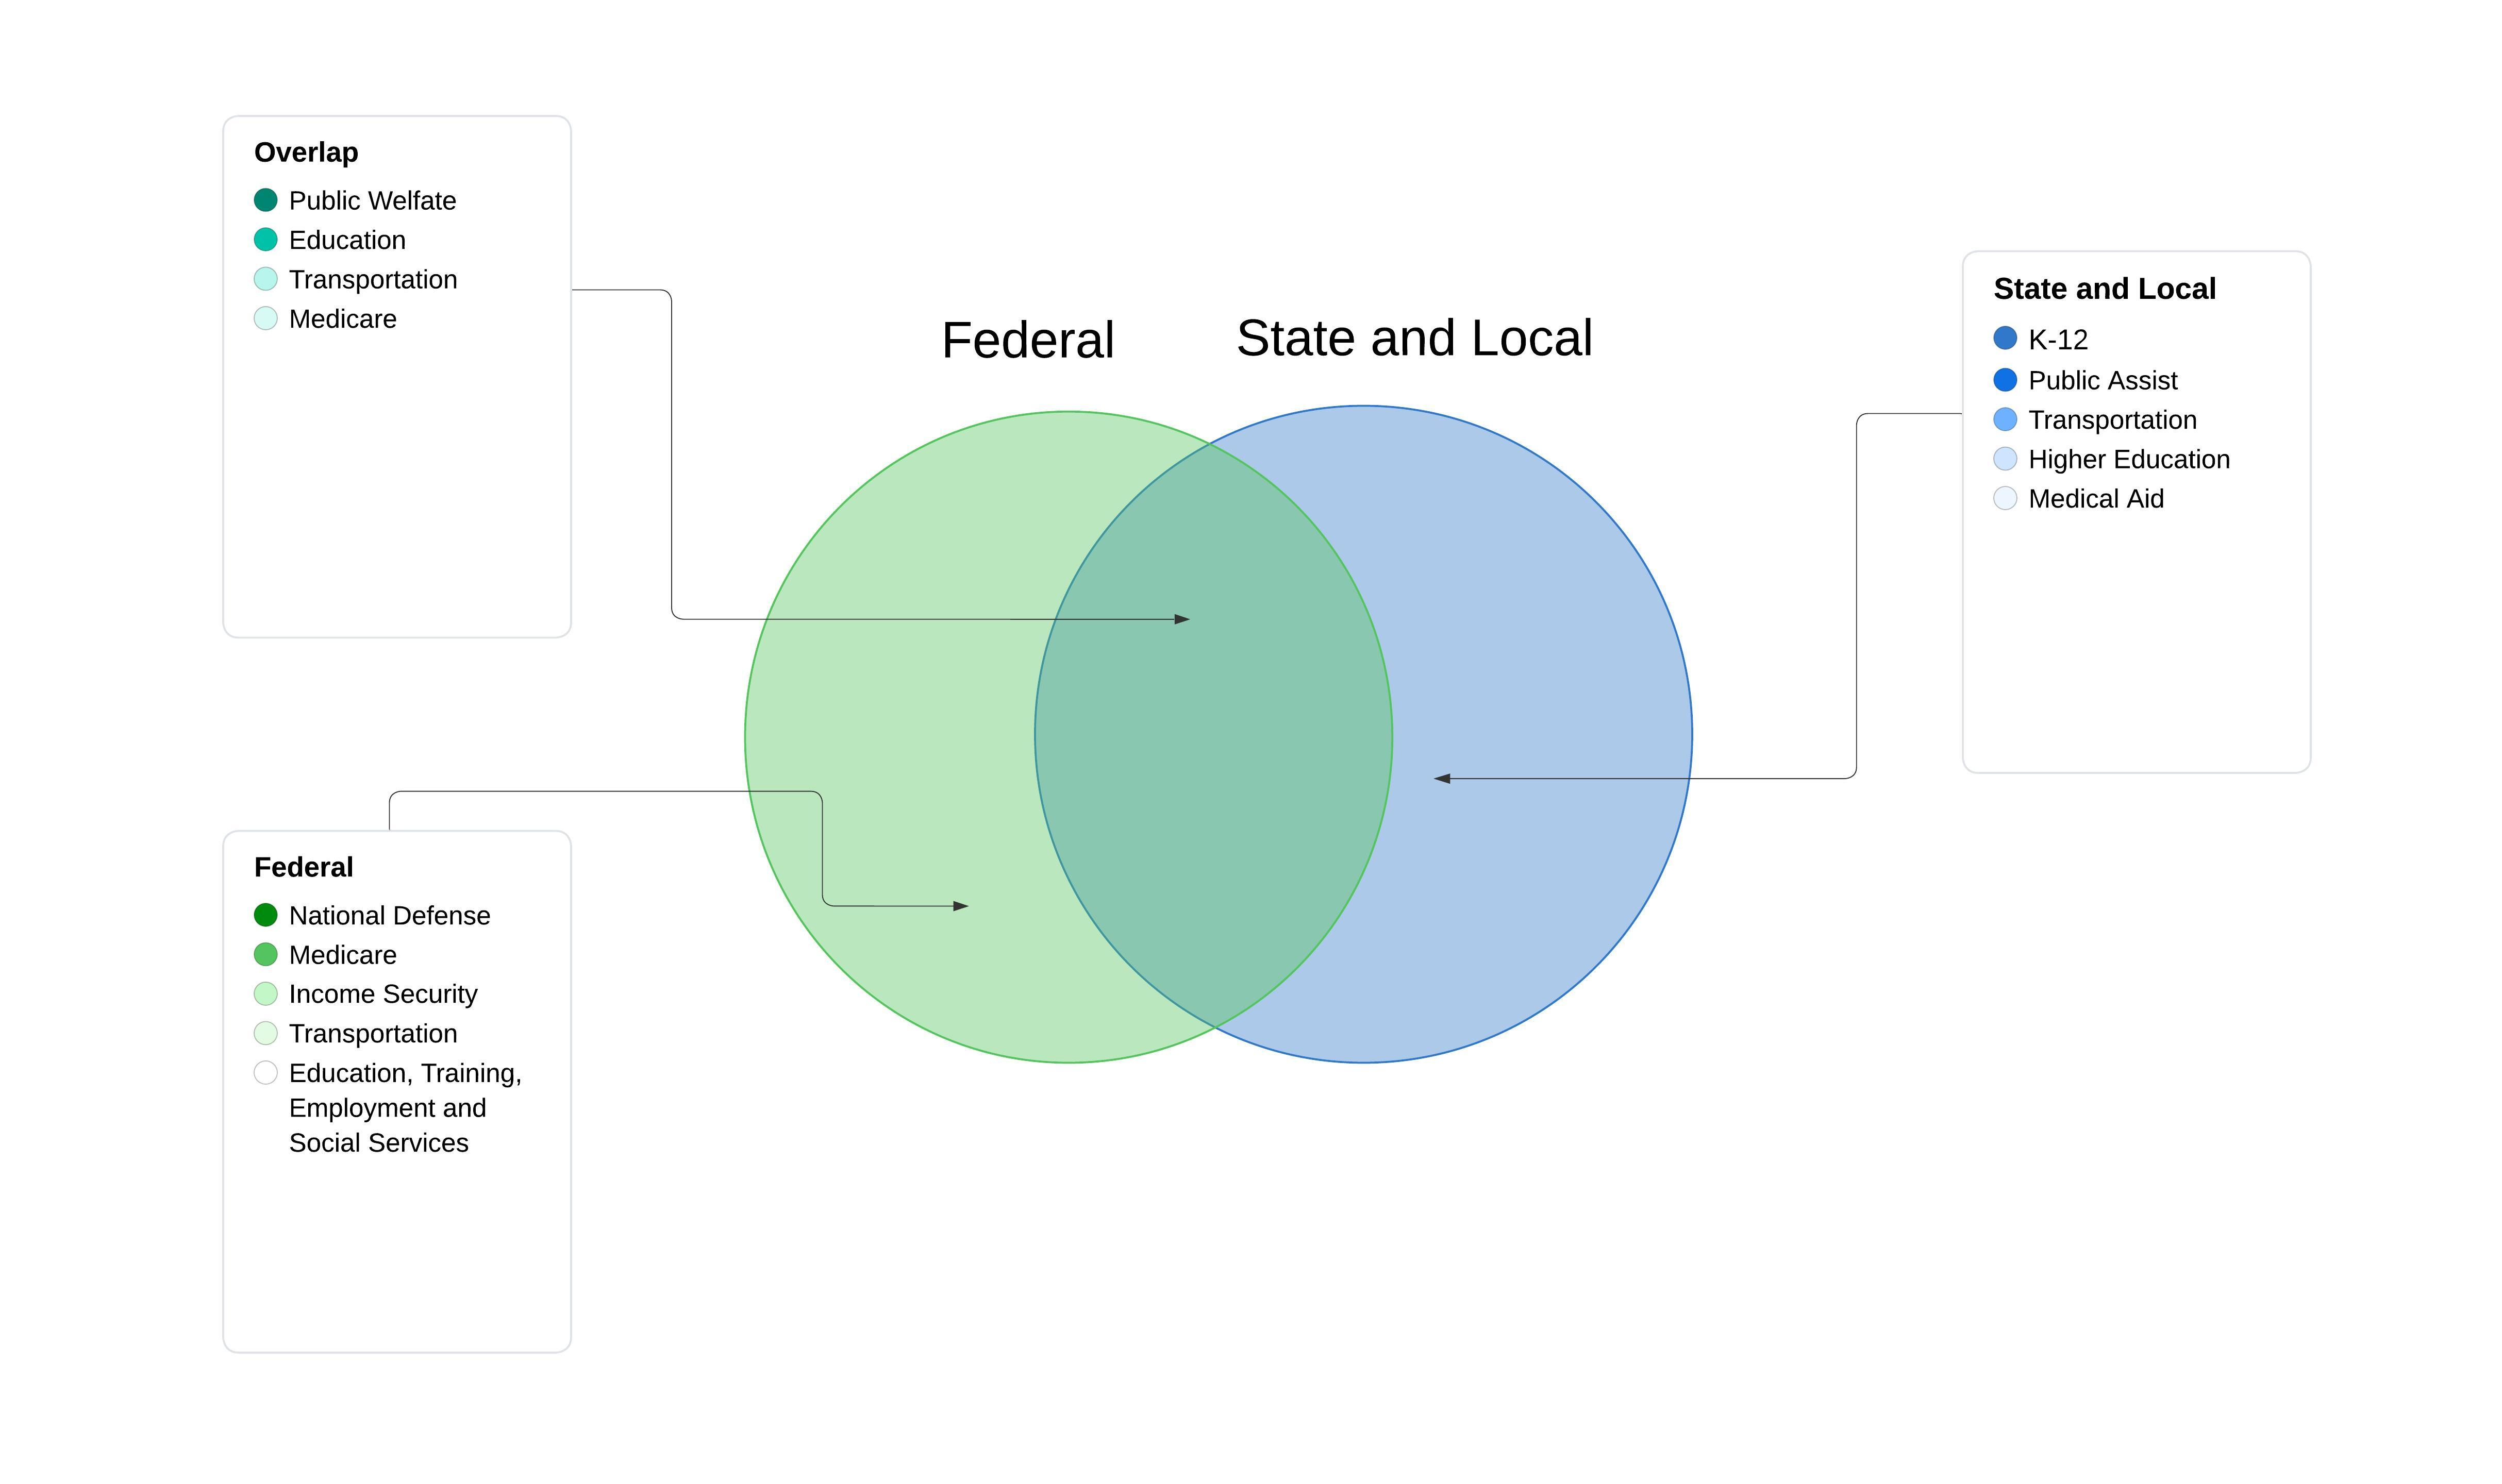
\includegraphics[scale=0.4]{Chapter-1/Figures/Venn graph on public goods.jpeg}
    \caption[Venn graph on public goods and services supplying]{Venn graph on public goods and services supplying by federal, states and local government
        \texttt{} }
    \label{Figure 1.4}
\end{figure}

\clearpage

\section{Chapter 2}

\begin{landscape}
    \begin{figure}[H]
        \centering
        \includegraphics[scale=0.045]{Chapter-2/Figures/tree.jpg}
        \caption[Dynamic Game Tree of 3 players]{Dynamic Game Tree between Central and Subnational Governments
            \texttt{} }
        \label{dynamicgamenoutility}
    \end{figure}
\end{landscape}
\newpage

\begin{figure}[htbp]
    \centering
    \subfigure[]{
        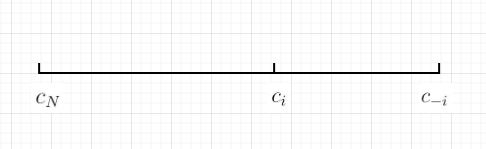
\includegraphics[width=0.61\textwidth]{Chapter-2/Figures/cncic-i.JPG}}
    \subfigure[]{
        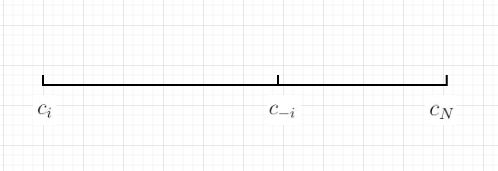
\includegraphics[width=0.61\textwidth]{Chapter-2/Figures/cic-icn.JPG}}
    \caption{When $c_N$ lies outside the range of $c_i$ and $c_{-i}$}
    \label{cnci}
\end{figure}

\begin{figure}[htbp]
    \centering
    \subfigure[]{
        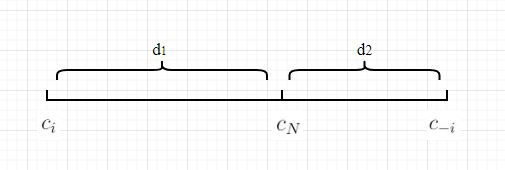
\includegraphics[width=0.71\textwidth]{Chapter-2/Figures/cicnc-i.JPG}}
    \subfigure[]{
        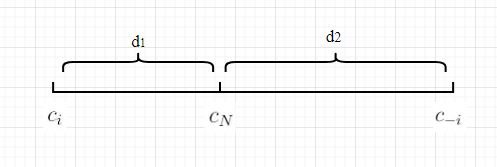
\includegraphics[width=0.71\textwidth]{Chapter-2/Figures/cicnc-i2.JPG}}
    \caption{When $c_N$ lies between $c_i$ and $c_i$}
    \label{cnci2}
\end{figure}
\clearpage
\section{Chapter 3}
\begin{figure}[H]
    \centering
    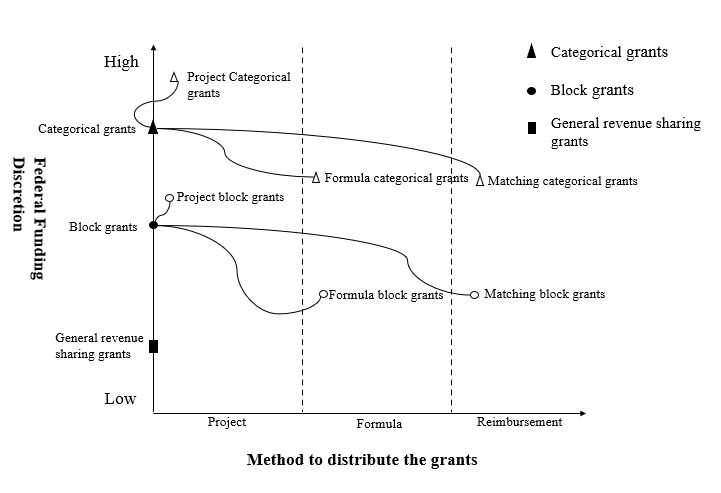
\includegraphics[scale=0.8]{Chapter-3/Figures/grants type.JPG}
    \caption[Grants Type in America]{Grants Type in America
        \texttt{} }
    \label{grantstype}
\end{figure}

% \begin{figure}[H]
%     \centering
%     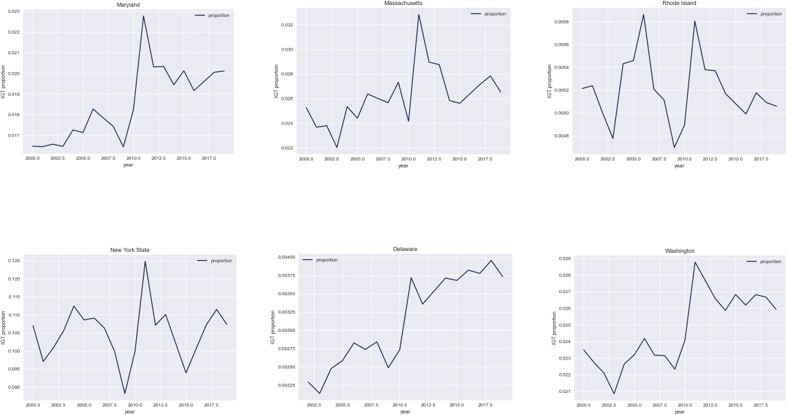
\includegraphics[scale=0.7]{Appendix-A/democratic.jpg}
%     \caption[Time Series Graph of Democratic States IGT(2000-2019)]{Time Series Graph of Democratic States IGT (2000-2019)
%         \texttt{} }
%     \label{Figure A.3}
% \end{figure}

% \begin{figure}[H]
%     \centering
%     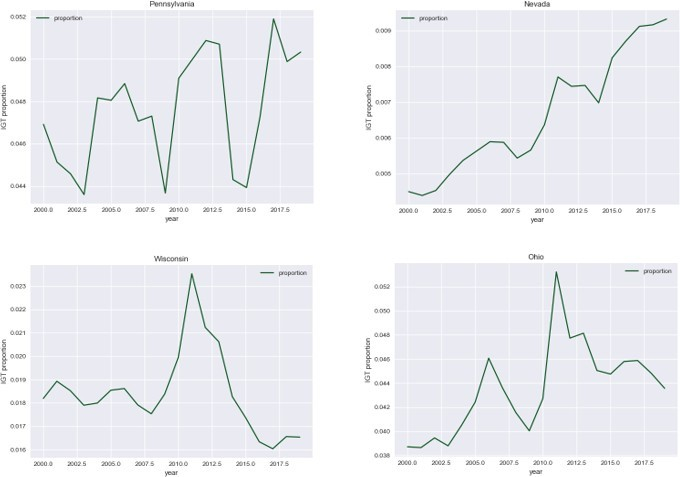
\includegraphics[scale=0.7]{Appendix-A/swing.jpg}
%     \caption[Time Series Graph of Swing States IGT (2000-2019) ]{Time Series Graph of Swing States IGT (2000-2019)
%         \texttt{} }
%     \label{Figure A.4}
% \end{figure}

\clearpage
\begin{figure}[H]
    \centering
    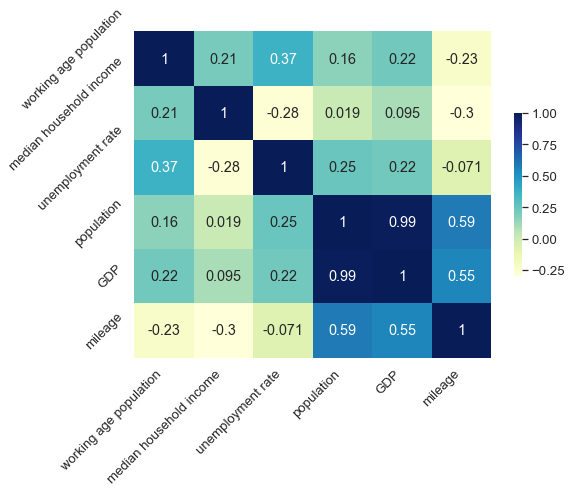
\includegraphics[scale=0.7]{Chapter-3/Figures/heatmap.png}
    \caption[Heatmap of the Social Characteristics]{Heatmap of the Social Characteristics
        \texttt{} }
    \label{heatmap}
\end{figure}
\clearpage

\begin{figure}[H]
    \centering  %居中
    \subfigure[Histgram]{   %第一张子图
        \begin{minipage}{7cm}
            \centering    %子图居中
            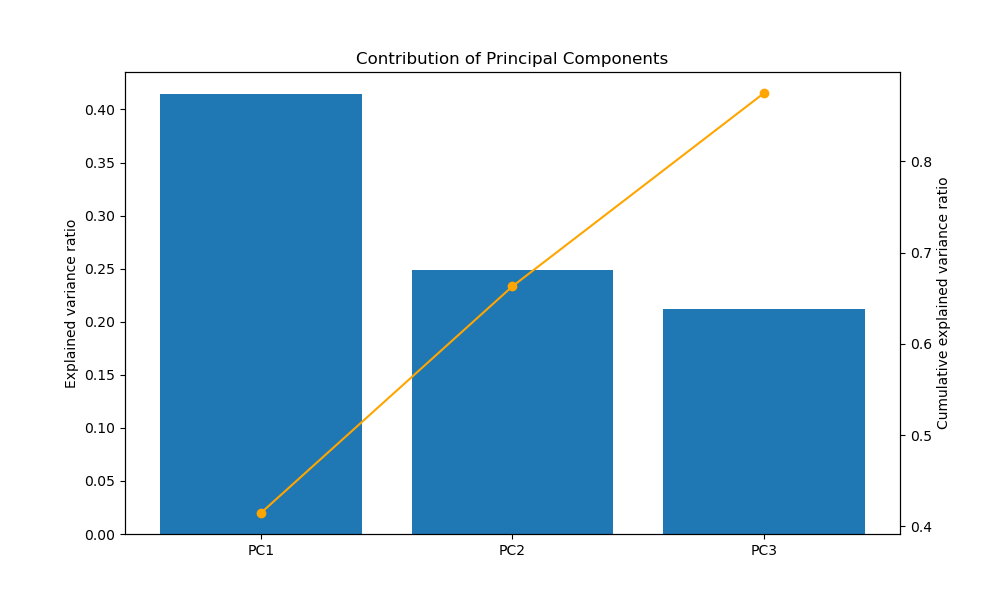
\includegraphics[scale=0.2]{Chapter-3/Figures/contribution.png}  %以pic.jpg的0.5倍大小输出
        \end{minipage}
    }
    \subfigure[Line]{ %第二张子图
        \begin{minipage}{7cm}
            \centering    %子图居中
            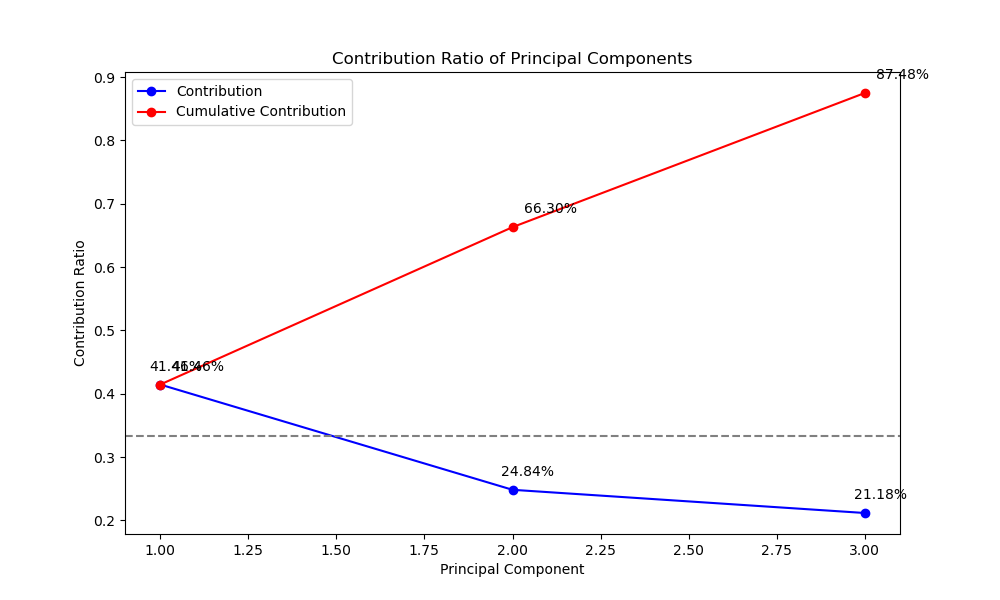
\includegraphics[scale=0.2]{Chapter-3/Figures/contribution2.png}%以pic.jpg的0.5倍大小输出
        \end{minipage}
    }
    \caption[Principle Components Contribution]{Principle Components Contribution}    %大图名称
    \label{principlecomponentcontribution}    %图片引用标记
\end{figure}
\clearpage


\begin{figure}[H]
    \centering  %居中
    \subfigure[2 Principle Components Analysis Scatter]{   %第一张子图
        \begin{minipage}{7cm}
            \centering    %子图居中
            \includegraphics[scale=0.45]{Chapter-3/Figures/pca.png}  %以pic.jpg的0.5倍大小输出
        \end{minipage}
    }
    \subfigure[3 principle Components Analysis Scatter]{ %第二张子图
        \begin{minipage}{7cm}
            \centering    %子图居中
            \includegraphics[scale=0.45]{Chapter-3/Figures/pca_3d.png}%以pic.jpg的0.5倍大小输出
        \end{minipage}
    }
    \caption[Principle Components Analysis Scatter Plot]{Social Characteristics Principle Components Analysis Scatter Plot}    %大图名称
    \label{Figure 2.2}    %图片引用标记
\end{figure}
\clearpage
\begin{figure}[H]
    \centering
    \includegraphics[scale=1]{Chapter-3/Figures/IGT and factors.jpg}
    \caption[IGT and Factors Scatter Plot]{Factor and IGT Scatter Plot
        \texttt{} }
    \label{Figure 2.3}
\end{figure}

\clearpage

\section{Chapter 4}

\begin{figure}[H]
    \centering
    \includegraphics[scale=0.4]{Chapter-4/Figures/Effect of Intergovernmental Transfer.jpeg}
    \caption{Effect of Intergovernmental Transfer
        \texttt{} }
    \label{Figure 3.1}
\end{figure}
\clearpage
\begin{figure}[H]
    \centering
    \includegraphics[scale=0.4]{Chapter-4/Figures/mfyeffect.jpg}
    \caption[Income Effect and Price Effect of Matching and Non-matching Grants]{Income Effect and Price Effect of Matching and Non-matching Grants
        \texttt{} }
    \label{Figure 3.3}
\end{figure}

\clearpage

\begin{figure}[H]
    \centering
    \includegraphics[scale=0.4]{Chapter-4/Figures/budget constrain distortion.jpg}
    \caption[Hamilton's Curved Budget Constraint]{Hamilton's Curved Budget Constrain
        \texttt{} }
    \label{Figure 3.4}
\end{figure}

\clearpage

\begin{figure}[htbp]
    \centering
    \subfigure[]{
        \includegraphics[width=0.45\textwidth]{Chapter-4/Figures/distofp1.jpg}}
    \subfigure[]{
        \includegraphics[width=0.45\textwidth]{Chapter-4/Figures/distofp2.jpg}}
    \subfigure[]{
        \includegraphics[width=0.45\textwidth]{Chapter-4/Figures/distofp3.jpg}}
    \subfigure[]{
        \includegraphics[width=0.45\textwidth]{Chapter-4/Figures/distofp4.jpg}}
    \caption{3-Dimensions Plot of the Fluctuation of Flypaper Effect under Distortion}
    \label{figfeunderdistortion}
\end{figure}

\clearpage

\begin{figure}[H]
    \centering
    \subfigure[$\beta=0.1$]{
        \includegraphics[width=0.45\textwidth]{Chapter-4/Figures/beta01.jpg}}
    \subfigure[$\beta=0.4$]{
        \includegraphics[width=0.45\textwidth]{Chapter-4/Figures/beta04.jpg}}
    \subfigure[$\beta=0.7$]{
        \includegraphics[width=0.45\textwidth]{Chapter-4/Figures/beta07.jpg}}
    \subfigure[$\beta=0.9$]{
        \includegraphics[width=0.45\textwidth]{Chapter-4/Figures/beta09.jpg}}
    \caption{2-Dimensions Plot of the Fluctuation of Flypaper Effect on $\alpha$}
    \label{fealpha}
\end{figure}
\clearpage
\begin{figure}[H]
    \centering
    \subfigure[$\alpha=0.1$]{
        \includegraphics[width=0.45\textwidth]{Chapter-4/Figures/alpha01.jpg}}
    \subfigure[$\alpha=0.4$]{
        \includegraphics[width=0.45\textwidth]{Chapter-4/Figures/alpha04.jpg}}
    \subfigure[$\alpha=0.7$]{
        \includegraphics[width=0.45\textwidth]{Chapter-4/Figures/alpha07.jpg}}
    \subfigure[$\alpha=0.9$]{
        \includegraphics[width=0.45\textwidth]{Chapter-4/Figures/alpha09.jpg}}
    \caption{2-Dimensions Plot of the Fluctuation of Flypaper Effect on $\beta$}
    \label{febeta}
\end{figure}
\clearpage
\section{Chapter 5}

\begin{figure}[H]
    \centering
    \includegraphics[scale=0.8]{Chapter-5/Figures/calculation effortttt.JPG}
    \caption[Expression of $\frac{\partial e_{i,t}}{\partial n}$]{Expression of $\frac{\partial e_{i,t}}{\partial n}$
        \texttt{} }
    \label{enenen}
\end{figure}

\clearpage

\begin{figure}[H]
    \centering
    \includegraphics[scale=0.7]{Chapter-5/Figures/laffer.jpg}
    \caption[Laffer Curve for Tax Collection Effort]{Laffer Curve for Tax Collection Effort
        \texttt{} }
    \label{laffer}
\end{figure}

\clearpage
\begin{figure}[H]
    \centering
    \includegraphics[scale=0.8]{Chapter-5/Figures/int_gen_W.jpg}
    \caption[Interaction effect between general transfer ratio and W-preference]{Interaction effect between general trnasfer ratio and W-preference
        \texttt{} }
    \label{int_gen_W}
\end{figure}

\begin{figure}[H]
    \centering
    \includegraphics[scale=0.8]{Chapter-5/Figures/inter_cons_W.jpg}
    \caption[Interaction effect between productive categorical transfer ratio and W-preference]{Interaction effect between productive categorical transfer ratio and W-preference
        \texttt{} }
    \label{int_cons_W}
\end{figure}

    % !TEX root = ../YourName-Dissertation.tex
\Appendix{Appendix for the proof}
*The proof is supplied in separate file.
\section{Proof of the Equalization Effect of General Transfer}

\section{Proof of the Free Rider Effect under Inaccurate Ascribe}


    % !TEX root = ../YourName-Dissertation.tex
\Appendix{Title of the Fourth Appendix}

\section{Introduction}
When in the Course of human events, it becomes necessary for one people  to dissolve the political bands which have connected them with another,  and to assume among the powers of the earth, the separate and equal station  to which the Laws of Nature and of Nature's God entitle them, a decent respect to the opinions of mankind requires that they should declare  the causes which impel them to the separation.

\section{More Declaration}

We hold these truths to be self-evident, that all men are created equal,  that they are endowed by their Creator with certain unalienable Rights,  that among these are Life, Liberty and the pursuit of Happiness. --That to secure these  rights, Governments are instituted among Men, deriving their just powers  from the consent of the governed, --That whenever any Form of Government  becomes destructive of these ends, it is the Right of the People to alter  or to abolish it, and to institute new Government, laying its foundation on  such principles and organizing its powers in such form, as to them shall  seem most likely to effect their Safety and Happiness. Prudence, indeed, will dictate that Governments long established should not  be changed for light and transient causes; and accordingly all experience  hath shewn, that mankind are more disposed to suffer, while evils are  sufferable, than to right themselves by abolishing the forms to which they  are accustomed. But when a long train of abuses and usurpations, pursuing invariably the same  Object evinces a design to reduce them under absolute Despotism, it is their  right, it is their duty, to throw off such Government, and to provide new Guards for their future security. --Such has been the patient sufferance of these Colonies; and such is now the  necessity which constrains them to alter their former Systems of Government.  The history of the present King of Great Britain [George III] is a history  of repeated injuries and usurpations, all having in direct object the  establishment of an absolute Tyranny over these States. To prove this, let Facts be submitted to a candid world.
    % !TEX root = ../YourName-Dissertation.tex
\Appendix{Title of the Fifth Appendix}

\section{Introduction}
When in the Course of human events, it becomes necessary for one people  to dissolve the political bands which have connected them with another,  and to assume among the powers of the earth, the separate and equal station  to which the Laws of Nature and of Nature's God entitle them, a decent respect to the opinions of mankind requires that they should declare  the causes which impel them to the separation.


    %%%%%%%%%%%%%%%%%%%%%%%%%%%%%%%%%%%%%%%%%%%%%%%%%%%%%%%%%%%%%%%
    % ESM students need to include a Nontechnical Abstract as the %
    % last appendix.                                              %
    %%%%%%%%%%%%%%%%%%%%%%%%%%%%%%%%%%%%%%%%%%%%%%%%%%%%%%%%%%%%%%%
    % This \include command should point to the file containing
    % that abstract.
    %\include{nontechnical-abstract}
    %%%%%%%%%%%%%%%%%%%%%%%%%%%%%%%%%%%%%%%%%%%
} % End of the \allowdisplaybreak command %
%%%%%%%%%%%%%%%%%%%%%%%%%%%%%%%%%%%%%%%%%%%

%%%%%%%%%%%%%%%%
% BIBLIOGRAPHY %
%%%%%%%%%%%%%%%%
% You can use BibTeX or other bibliography facility for your
% bibliography. LaTeX's standard stuff is shown below. If you
% bibtex, then this section should look something like:
\begin{singlespace}
    \bibliographystyle{GLG-bibstyle}
    \addcontentsline{toc}{chapter}{Bibliography}
    \bibliography{Biblio-Database}
\end{singlespace}

%\begin{singlespace}
%\begin{thebibliography}{99}
%\addcontentsline{toc}{chapter}{Bibliography}
%\frenchspacing

%\bibitem{Wisdom87} J. Wisdom, ``Rotational Dynamics of Irregularly Shaped Natural Satellites,'' \emph{The Astronomical Journal}, Vol.~94, No.~5, 1987  pp. 1350--1360.

%\bibitem{G&H83} J. Guckenheimer and P. Holmes, \emph{Nonlinear Oscillations, Dynamical Systems, and Bifurcations of Vector Fields}, Springer-Verlag, New York, 1983.

%\end{thebibliography}
%\end{singlespace}

\backmatter

% Vita
\vita{SupplementaryMaterial/Vita}

\end{document}

